% for a more compact document, add the option openany to avoid
%starting all chapters on odd numbered pages
\documentclass[12pt, draft]{cmuthesis}

\usepackage{comment}
\usepackage{url}
\usepackage{ifthen}
\usepackage{framed}
\usepackage{multirow}
\usepackage{subcaption}
\usepackage{times}
\usepackage{amssymb}
\usepackage[export]{adjustbox}
\usepackage{rotating}
% \usepackage{times}
\usepackage{fullpage}
\usepackage{amsmath}
\usepackage[numbers,sort]{natbib}
\usepackage[backref,pageanchor=true,plainpages=false, pdfpagelabels, bookmarks,bookmarksnumbered,
%pdfborder=0 0 0,  %removes outlines around hyper links in online display
]{hyperref}
% \usepackage{subfigure}
\usepackage{color,soul,xspace}
\usepackage{makecell}
\usepackage{booktabs}
\usepackage{graphicx}


%% fix the conflict between times and new acmart template
% \renewcommand{\textrightarrow}{$\rightarrow$}

%%%
%%%  Comments
%%%
\newcommand{\showComments}{yes}
\newcommand{\note}[2]{
	\ifthenelse{\equal{\showComments}{yes}}{\textcolor{#1}{#2}}{}
}

\newcommand{\showRevision}{no}
\newcommand{\revision}[1]{
	\ifthenelse{\equal{\showRevision}{yes}}{\textcolor{red}{#1}}{#1}
}


\newcommand{\TODO}[1]{\note{red}{#1}}


% FOR SUBMISSION ONLY: Eliminate copyright box at bottom of first page
% Use \toappear{} if you want a blank ACM copyright box instead of suppressing it
\usepackage{etoolbox}
\makeatletter
\patchcmd{\maketitle}{\@copyrightspace}{}{}{}
\makeatother


% Itemize and Enumerate with less white space wasted
\newenvironment{smitemize}%
  {\begin{list}{$\bullet$}%
     {\setlength{\parsep}{1pt}%
      \setlength{\topsep}{1pt}%
      \setlength{\itemsep}{1pt}}}%
  {\end{list}}

\newenvironment{smenumerate}{
\begin{enumerate}
  \setlength{\itemsep}{2.5pt}
  \setlength{\parskip}{0pt}
  \setlength{\parsep}{0pt}
}{\end{enumerate}}

\newenvironment{mypara}{
   \vspace{0.1in}
   \textbf}
{\plain}


\newcommand{\lc}[1]{\lowercase{#1}}
\newcommand{\uc}[1]{\uppercase{#1}}
\newcommand{\xc}[1]{\small\sc #1}
\usepackage{epsfig}


\newenvironment{captiontext}{%
   \par\vspace{0.1in}\renewcommand{\baselinestretch}{0.9}\footnotesize}%
   {\renewcommand{\baselinestretch}{1.0}\par}


%
% defining the \BibTeX command - from Oren Patashnik's original BibTeX documentation.
\def\BibTeX{{\rm B\kern-.05em{\sc i\kern-.025em b}\kern-.08emT\kern-.1667em\lower.7ex\hbox{E}\kern-.125emX}}

\usepackage{setspace} % for \onehalfspacing and \singlespacing macros
\usepackage{etoolbox}
\AtBeginEnvironment{quote}{\singlespacing\small}

% \settopmatter{printacmref=false} % Removes citation information below abstract
% \renewcommand\footnotetextcopyrightpermission[1]{} % removes footnote with conference information in first column
% \pagestyle{plain}


% Abbreviations


% Approximately 1" margins, more space on binding side
%\usepackage[letterpaper,twoside,vscale=.8,hscale=.75,nomarginpar]{geometry}
%for general printing (not binding)
\usepackage[letterpaper,twoside,vscale=.8,hscale=.75,nomarginpar,hmarginratio=1:1]{geometry}

% Provides a draft mark at the top of the document. 
\draftstamp{\today}{DRAFT}

\begin{document} 
\frontmatter

\begin{document} 

\frontmatter

\title{
{\bf Scaling Wearable Cognitive Assistance}}
\author{Junjue Wang \\ \href{mailto:junjuew@cs.cmu.edu}{junjuew@cs.cmu.edu}}
\date{June 2018}
\Year{2018}
\trnumber{}

\vspace{3cm}

% \begin{dedication}
% \end{dedication}

\committee{
Mahadev Satyanarayanan (Satya) (Chair) \\
Daniel Siewiorek \\
Martial Hebert \\
Roberta Klatzky \\
Padmanabhan Pillai (Intel Labs)
}

\support{}
\disclaimer{}

% copyright notice generated automatically from Year and author.
% permission added if \permission{} given.

\keywords{Wearable Cognitive Assistance, Edge Computing, Cloudlet, Scalability}

\maketitle


\pagestyle{plain} % for toc, was empty

%% Obviously, it's probably a good idea to break the various sections of your thesis
%% into different files and input them into this file...

%% \begin{abstract}
%% A short summary.
%% \end{abstract}

%% \begin{acknowledgments}
%% \end{acknowledgments}

\clearpage

\tableofcontents
%% \listoffigures
%% \listoftables
\mainmatter
%% Double space document for easy review:
%\renewcommand{\baselinestretch}{1.66}\normalsize

% The other requirements Catherine has:
%
%  - avoid large margins.  She wants the thesis to use fewer pages, 
%    especially if it requires colour printing.
%
%  - The thesis should be formatted for double-sided printing.  This
%    means that all chapters, acknowledgements, table of contents, etc.
%    should start on odd numbered (right facing) pages.
%
%  - You need to use the department standard tech report title page.  I
%    have tried to ensure that the title page here conforms to this
%    standard.
%
%  - Use a nice serif font, such as Times Roman.  Sans serif looks bad.
%
% Other than that, just make it look good...

\chapter{Introduction}

It has been a long endeavour to augment human cognition with machine
intelligence. As early as in 1945, Vannevar Bush envisioned a machine Memex that
provides "enlarged intimate supplement to one's memory" and can be "consulted
with exceeding speed and flexibility" in the seminal article \textit{As We May
Think}~\cite{bush1945we}. This vision has been brought closer to reality by years
of research in computing hardware, artificial intelligence, and human-computer
interaction. In late 90s to early 2000s, Smailagic et al
~\cite{smailagic1993case}~\cite{smailagic1998very}~\cite{smailagic2002application}
created prototypes of wearable computers to assist several cognitive tasks, for
example, displaying inspection manuals in a head-up screen to facilitate
aircraft maintenance. Around the same time, Loomis el
al~\cite{loomis1998navigation}~\cite{loomis1994personal} explored using
computers carried in a backpack to help the blind navigate through auditory
cues. Davis et al~\cite{davies1998developing} developed a context-sensitive
intelligent visitor guide leveraging hand-portable multimedia systems. While
these research work pioneered human cognition assistance, they are limited by
the technologies of their time.

More recently, as many underlying technologies experience fundamental changes,
new genres of several applications have been 

advancement in machine learning, especially in machine
learning, computer hardware, and distributed computing. Many applications that
have been built for

(Challenges of making them happen)

Despite the ventures of these research work, we are still far from the reality
that human augmentation is prevalent in society. A mature cognitive system needs
three key components. (algorithm, compute, networking)

(Recent wonderful advancement has made the dream closer)
In recent five years, significant improvements have made WCA feasible. (DNN,
edge computing, and wearable h/w).

(At the intersection of all three, WCA has been shown feasiblity emerged)
Wearable Cognitive Assistance has emerged as a new genre of applications that
pushes the boundaries of augmented cognition. These applications continuously
process data from body-worn sensors and provide just-in-time guidance to help a
user complete a specific task. For example, an IKEA Lamp
assistant~\cite{chen2018application} has been built to assist the assembly of a
table lamp. To use the application, a user wears a head-mounted smart glass that
continuously captures her actions and surroundings from a first-person
viewpoint. In real-time, the camera stream is analyzed to identify the state of
the assembly. Audiovisual instructions are generated based on the detected
state. The instructions either demonstrate a subsequent procedure or alert and
correct a mistake.

(WCA has its root in edge computing)
Edge system

(Problems that have not been addressed)

(scalability at the edge)

(scalability for development)
Fundamental changes in development. uncertainty. Fundamental changes in how
people deploy applications.

Although Wearable Cognitive Assistance shares the vision of cognition
enhancement with many previous research
efforts~\cite{kidd1999aware}~\cite{loomis1998navigation}
~\cite{cheverst2000developing}~\cite{tanuwidjaja2014chroma},
its design goals advance the frontier of mobile computing in multiple aspects.
First, wearable devices, particularly head-mounted smart glasses, are used to
reduce the discomfort caused by carrying a bulky computation device. Users are
freed from holding a smartphone and therefore able to interact with the physical
world using both hands. The convenience of this interaction model comes at the
cost of constrained computation resources. The small form-factor of smart
glasses significantly limits their onboard computation capability due to size,
cooling, and battery life reasons. Second, placed at the center of computation
is the unstructured high-dimensional image and video data. Only these data types
can satisfy the need to extract rich semantic information to identify the
progress and mistakes a user makes. Furthermore, state-of-art computer vision
algorithms used to analyze image data are both compute-intensive and challenging
to develop. Third, many cognitive assistants give real-time feedback to users
and have stringent end-to-end latency requirements. An instruction that arrives
too late often provides no value and may even confuse or annoy users. This
latency-sensitivity further increases their high demands of system resource and
optimizations.

To meet the latency and the compute requirements, previous research leverages
edge computing and offloads computation to a cloudlet. A
cloudlet~\cite{satyanarayanan2009case} is a small data-center located at the
edge of the Internet, one wireless hop away from users. Researchers have
developed an application framework for wearable cognitive assistance, named
Gabriel, that leverages cloudlets, optimizes for end-to-end latency, and eases
application
development~\cite{chen2018application}~\cite{ha2014towards}~\cite{chen2017empirical}.
On top of Gabriel, several prototype applications have been built, such as
Ping-Pong Assistance, Lego Assistance, Sandwich Assistance, and Ikea Lamp
Assembly Assistance. Using these applications as benchmarks,
~\cite{chen2017empirical} presents empirical measurements detailing the latency
contributions of individual system components. Furthermore, a multi-algorithm
approach was proposed to reduce the latency of computer vision computation by
executing multiple algorithms in parallel and conditionally selecting a fast and
accurate algorithm for the near future.

While previous research has demonstrated the technical feasibility of wearable
cognitive assistants and meeting latency requirements, many practical concerns
have not been addressed. First, previous work operates the wireless networks and
cloudlets at low utilization in order to meet application latency. The economics
of practical deployment preclude operation at such low utilization. In contrast,
resources are often highly utilized and congested when serving many users. How
to efficiently scale Gabriel applications to a large number of users remains to
be answered. Second, previous work on the Gabriel framework reduces application
development efforts by managing client-server communication, network flow
control, and cognitive engine discovery. However, the framework does not address
the most time-consuming parts of creating a wearable cognitive assistance
application. Experience has shown that developing computer vision modules that
analyze video feeds is a time-consuming and painstaking process that requires
special expertise and involves rounds of trial and error. Developer tools that
alleviate the time and the expertise needed can greatly facilitate the creation
of these applications.

The core contribution of this thesis is to holistic improve the scalability of
wearable cognitive assistance. Scalability, in this thesis, is considered from
three facets. First, from a traditional distributed system perspective, a
scalable system is one that enables most associated clients with fixed amount of
infrastructure and has ways to serve more clients as resources increase. Second,
we also want to enable small software development team to quickly create these
applications. Third, devOps should be able to easily deploy and manage
applications on the fly on a variety of hardware.

% 1. tradition meaning of enabling most associated
% clients with fixed amount of infrastructure 
% 2. enabling small software dev team
% to develop large suite of applications 
% 3. enabling small admin team to deploy a
% large collection of applications

% \section{Motivation}
% \subsection{Wearable Cognitive Assistance}
% \subsection{Use of Cloudlets}
% \subsection{Characteristics of Gabriel Applications}
% \section{Related Work, mostly Zhuo's work}
% \section{Approach}
\section{Thesis Statement}

My thesis is that these efforts can help to scale wearable cognitive assistance.
Notably, we claim that:

\textbf{Two critical challenges to the widespread adoption of wearable cognitive
  assistance are 1) the need to operate cloudlets and wireless network at low
  utilization to achieve acceptable end-to-end latency 2) the level of specialized
  skills and the long development time needed to create new applications. These
  challenges can be effectively addressed through system optimizations,
  functional extensions, and the addition of new software development tools to
  the Gabriel platform.}

\section{Thesis Overview}

The thesis is organized as follows.



% This proposal lays out my plan to address these challenges. In order to meet
% latency requirements when utilization is high, restricting the freedom of using
% resources while taking account of workload characteristics is needed. The scarce
% resource can either be the wireless links or the cloudlets. First, upload
% bandwidth in cellular networks is limited compared to download bandwidth and has
% high variance. Existing wireless infrastructure cannot afford to continuously
% stream high-definition videos from many users. I plan to address this problem
% with application-level mechanisms that exploit the attributes of the workload to
% reduce bandwidth consumption. Second, accelerators, such as GPUs, on cloudlets
% are both limited and heterogeneous. Due to the high demands of accelerators from
% state-of-art computer vision algorithms, the intelligent discovery of
% accelerator resources and the usage coordination among applications are required to
% serve more users. I plan to work on these problems in an edge computing context
% to address how to discover appropriate cloudlets for offload and how to
% coordinate among applications with different latency requirements to share
% scarce accelerators.

% In order to address the difficulty of development, I plan to build tools to
% reduce the expertise and time needed when creating wearable cognitive
% assistants. First, state-of-art computer vision uses Deep Neural Networks (DNNs)
% for critical tasks, including image classification, object detection, and
% semantic segmentation. DNNs champion end-to-end learning instead of hand-crafted
% features. The absence of manually created features provides an opportunity to
% build developer tools that replace ad-hoc trial and error development process.
% On the other hand, DNNs requires a significant amount of labeled data for training. I
% plan to build tools that help label examples and automate the creation of
% DNN-based object detectors.

\chapter{Background}
\label{chapter: background}

\section{Edge Computing}
\label{sec: bg-edge}

\begin{figure*}[t]
\begin{minipage}[c]{2.5in}
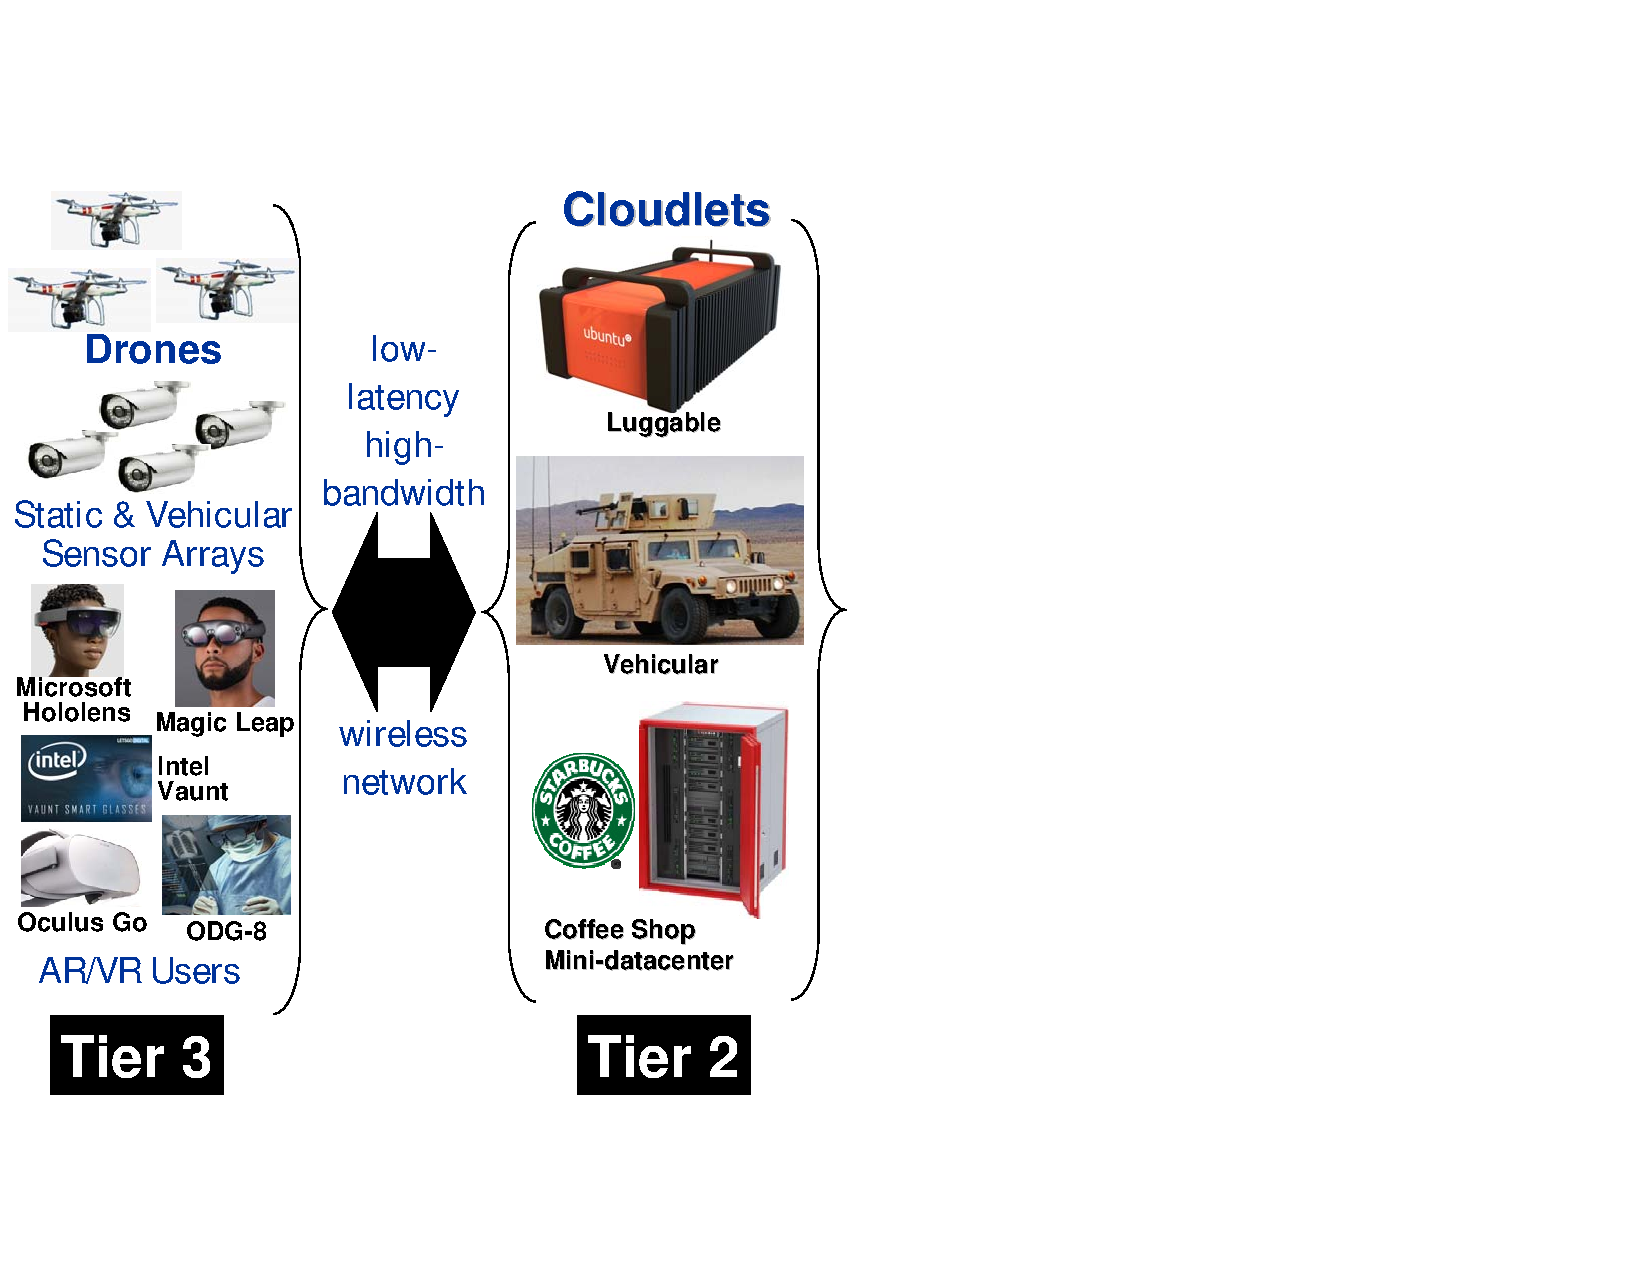
\includegraphics[scale=0.45]{FIGS/fig-3tier-A.pdf}
\end{minipage}
\begin{minipage}[c]{2.7in}
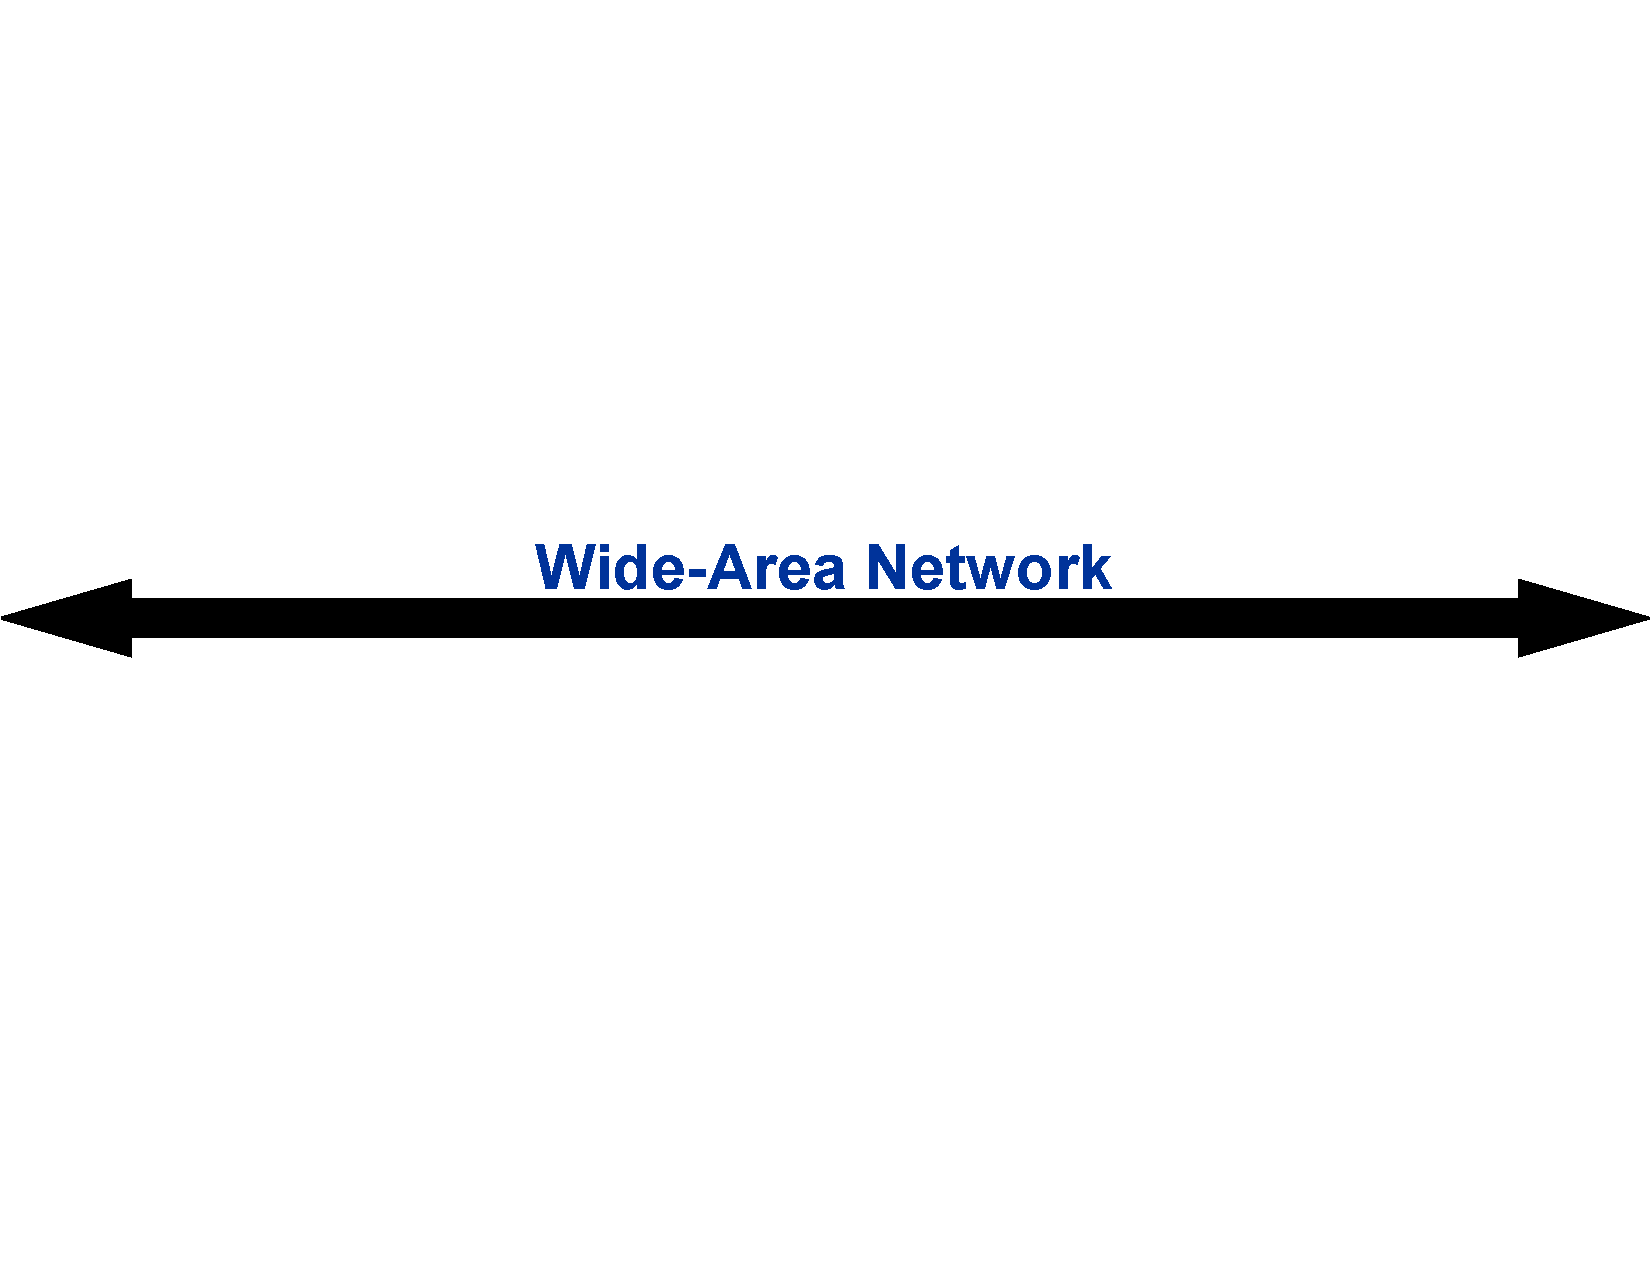
\includegraphics[scale=0.25]{FIGS/fig-3tier-B-cropped.pdf}\\
\end{minipage}
\begin{minipage}[c]{1in}
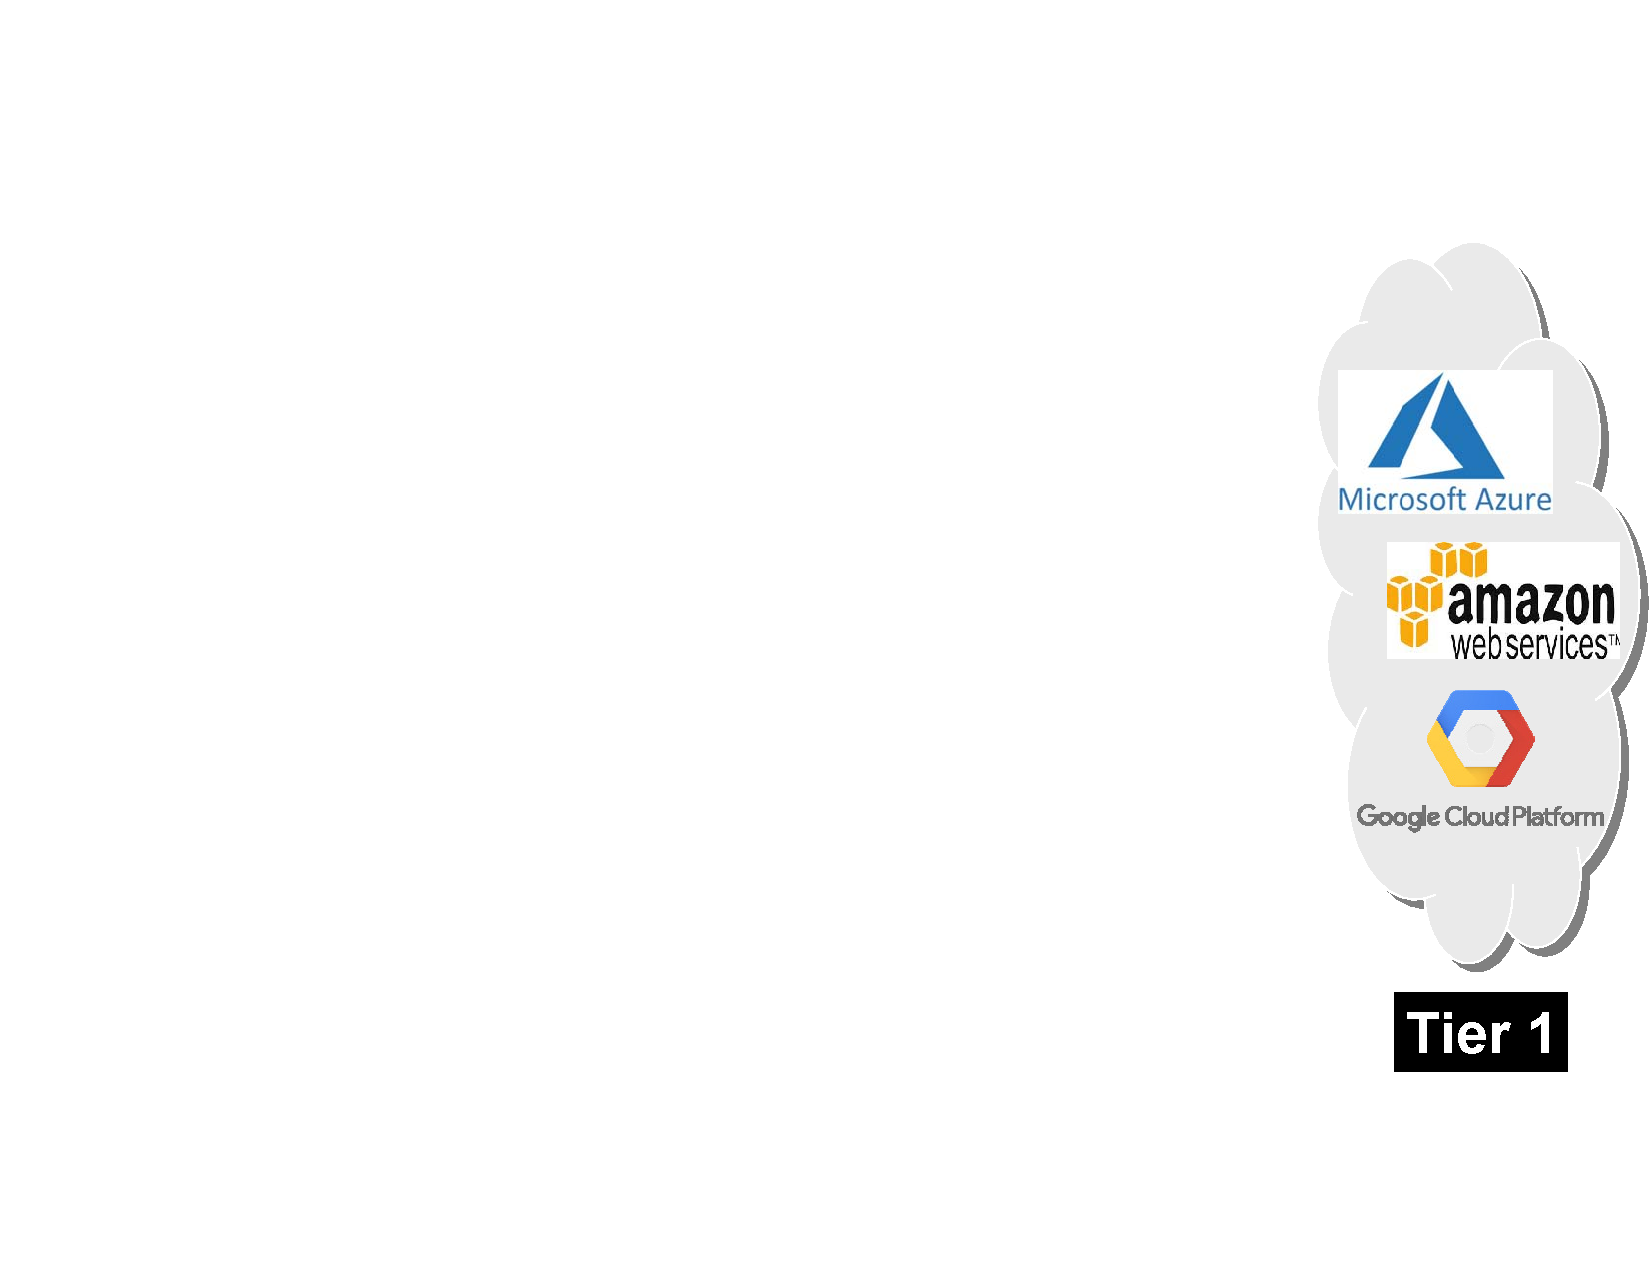
\includegraphics[scale=0.45]{FIGS/fig-3tier-C.pdf}
\end{minipage}
\centering
\captiontext{(Source: Satya et al~\cite{satya2019computing})}
\caption{\small Tiered Model of Computing}
\label{fig:3tier}
\end{figure*}

{\em Edge computing} is a nascent computing paradigm that has gained
considerable traction over the past few years. It champions the idea of placing
substantial compute and storage resources at the edge of the Internet, in close
proximity to mobile devices or sensors.  Terms such as
``cloudlets''~\cite{Satya2009}, ``micro data centers (MDCs)''~\cite{Greene2012},
``fog''~\cite{Bonomi2012}, and ``mobile edge computing (MEC)''~\cite{Brown2013}
are used to refer to these small, edge-located computing nodes.  We use these
terms interchangably in the rest of this dissertation. Edge computing is motivated by
its potential to improve latency, bandwidth, and scalability over a cloud-only
model.  More practically, some efforts stem from the drive towards
software-defined networking (SDN) and network function virtualization (NFV), and
the fact that the same hardware can provide SDN, NFV, and edge computing
services. This suggests that infrastructure providing edge computing services
may soon become ubiquitous, and may be deployed at greater densities than
content delivery network (CDN) nodes today. 

Satya et al.~\cite{satya2019computing} best describes the modern computing
landscape with edge computing using a tiered model, shown in
Figure~\ref{fig:3tier}. Tiers are separated by distinct yet stable sets of
design constraints. From left to right, this tiered model represents a hierarchy
of increasing physical size, compute power, energy usage, and elasticity. Tier-1
represents today's large-scale and heavily consolidated data-centers. Compute
elasticity and storage permanence are two dominating themes here. Tier-3
represents IoT and mobile devices, which are constrained by their physical size,
weight, and heat dissipation. Sensing is the key functionality of Tier-3
devices. For example, today's smartphones are already rich in sensors, including
camera, microphone, accelerometers, gyroscopes and GPS. In addition, an
increasing amount of IoT devices with specific sensing modalities are getting
adopted, e.g. smart speakers, security cameras, and smart thermostats. 

With the large-scale deployment of Tier-3 devices, there exists a tension
between the gigantic amount of data collected and generated by them and their
limited capabilities to process these data on-board. For example, most
surveillance cameras are limited in computation to run state-of-art computer
vision algorithms to analyze the videos they capture. To overcome this tension,
a tier-3 device could offload computation over network to tier-1. This
capability was first demonstrated in 1997 by Noble et al.~\cite{Noble1997}, who
used it to implement speech recognition with acceptable performance on a
resource-limited mobile device. In 1999, Flinn et al.~\cite{Flinn1999} extended
this approach to improve battery life.  These concepts were generalized in a
2001 paper that introduced the term {\em cyber foraging} for the amplification
of a mobile device's data or compute capabilities by leveraging nearby
infrastructure~\cite{Satya2001}.  Thanks to these research efforts, computation
offloading is widely used by IoT devices today. For example, when a user asks an
Amazon Echo smart speaker ``Alexa, what is the weather today?'', the user's
audio stream is captured by the smart speaker and transmitted to the cloud for
speech recognition, text understanding, and question answering.

However, offloading computation to the cloud has its own downside. Because of
the consolidation needed to achieve the economy of scale, today's datacenters
are ``far'' from tier-3 devices. The latency, throughput, and cost of wide-area
network (WAN) significantly limit the amount of applications that can benefit
from computation offloading. Even worse, it is the logical distance in the
network that matters rather than the physical distance. Routing decisions in
today's Internet are made locally and are based on business agreements,
resulting in suboptimal solutions. For example, using traceroute, we determine
that a LTE packet originating from a smartphone on the campus of Carnegie Mellon
University (CMU) in Pittsburgh to a nearby server actually traverses to
Philedelphia, a city several hundreds miles away. This is because Philidephia
has the nearest peering point of the particular commercial LTE network in use to
the public Internet. In 2010, Li et al.~\cite{li2010cloudcmp} report that the
average round trip time (RTT) from 260 global vantage points to their optimal
Amazon EC2 instances is 74 ms. In addition to long network delay, the high
network fan-in of datacenters means its aggregation network need to carry
significant amount of traffic. As the number of tier-3 devices is expected to
grow exponentially, these network links face significant challenges to handle
the ever-increasing volume of ingress traffic. 

\begin{figure}
\begin{minipage}[c]{3in}
\begin{center}
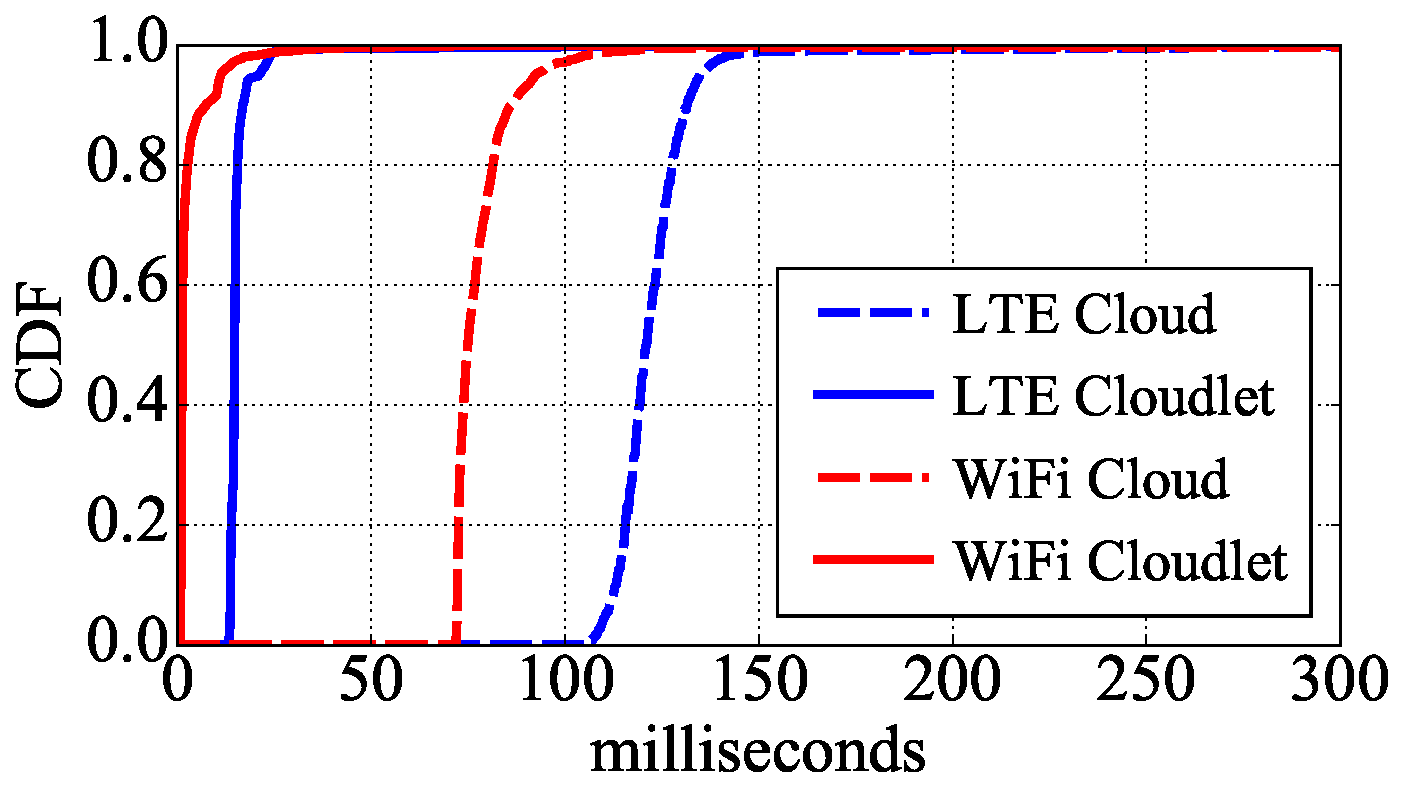
\includegraphics[height=1.5in]{FIGS/ping_cdf.pdf}
\captiontext{(Source: Hu et al~\cite{hu2016quantifying})}
\caption{CDF of pinging RTTs}
\label{fig:ping-CDF}
\end{center}
\end{minipage}
\begin{minipage}[c]{3.5in}
\begin{center}
    \hspace{0.2in}
    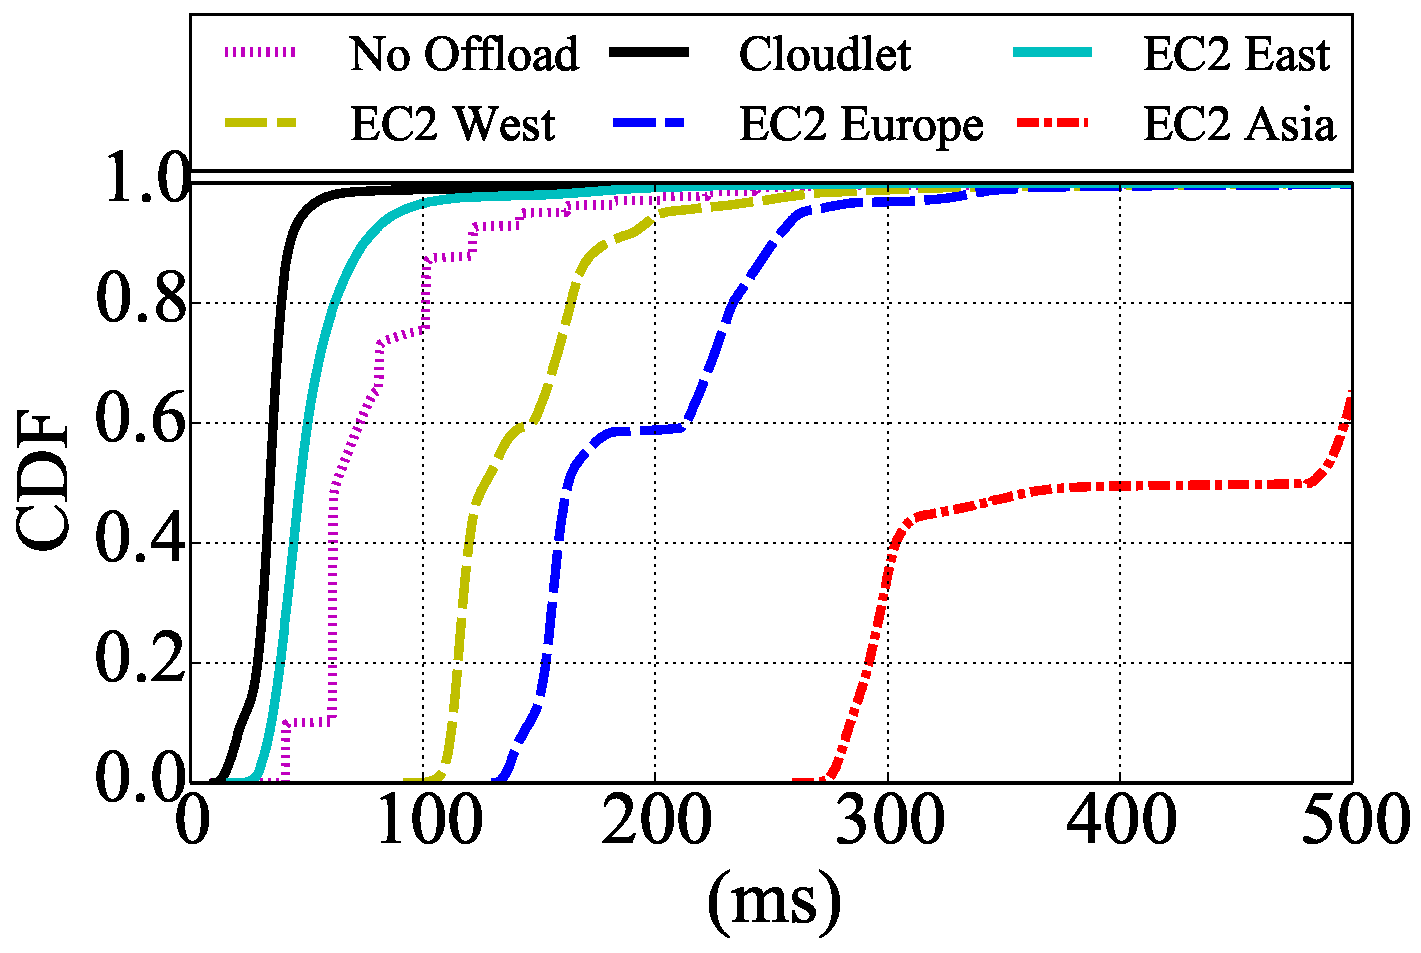
\includegraphics[width=0.8\textwidth,clip,trim=91pt 376pt 0 0]{FIGS/Legend-Wifi.pdf}
    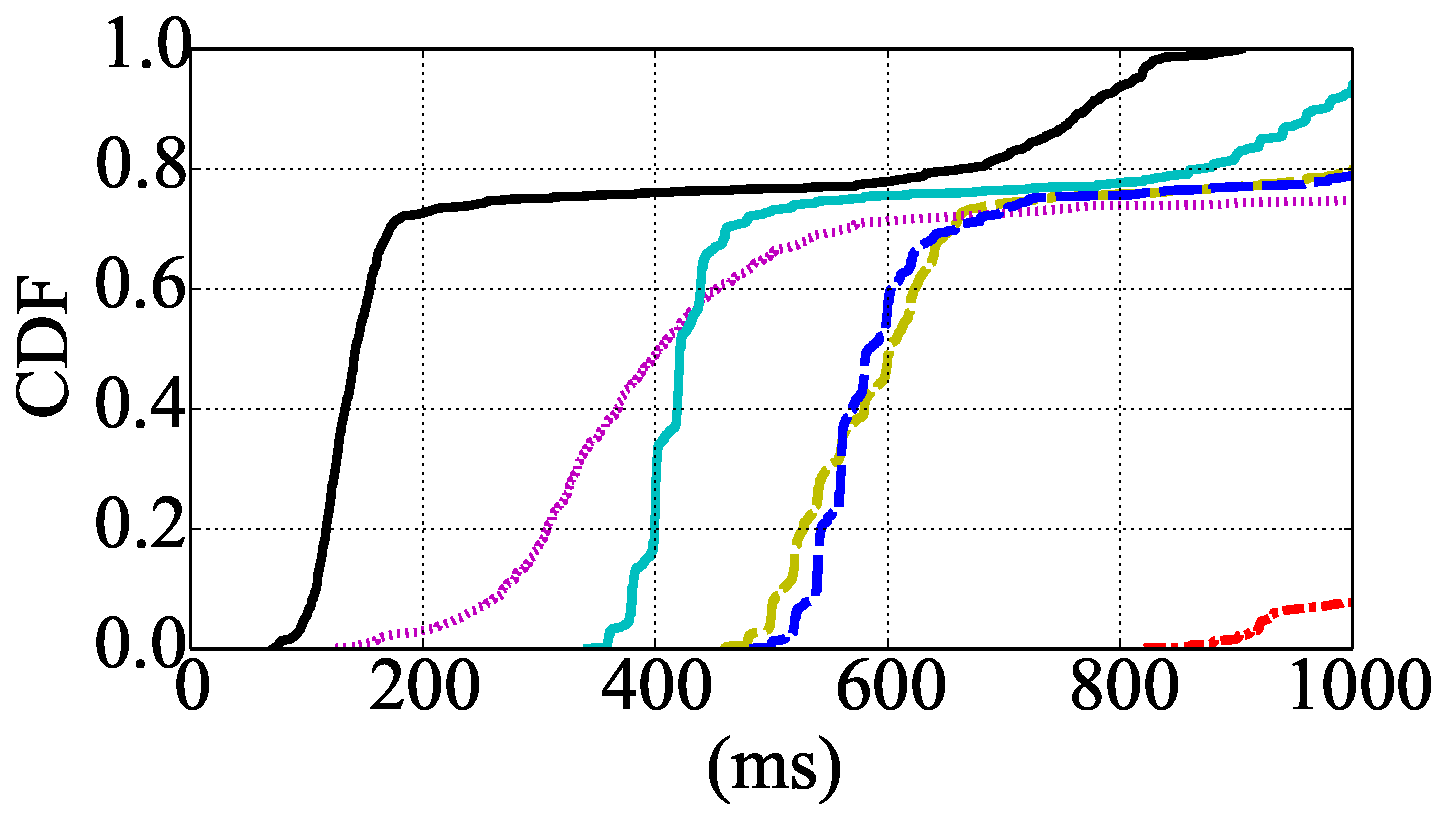
\includegraphics[width=3in]{FIGS/Face-LTE.pdf}
\captiontext{(Source: Hu et al~\cite{hu2016quantifying})}
\caption{FACE Response Time over LTE}
\label{fig:response-time-lte-face}
\end{center}
\end{minipage}
\end{figure}

To counter these problems, edge computing, shown as the tier-2 in
Figure~\ref{fig:3tier}, is proposed. Cloudlets at tier-2 creates the illusion of
bringing Tier-1 ``closer''. They are featured by their network proximity to
tier-3 devices and their significantly larger compute and storage compared to
tier-3 devices. While tier-3 devices typically run on battery and are optimized
for low energy consumption, saving energy is not a major concern for tier-2 as
they are either plugged into the electric grid or powered by other sources of
energy (e.g. fuels in a vehicle). Cloudlets serve two purposes in the tiered
model. First, they provide infrastructure for compute-intensive and
latency-sensitive applications for tier-3. Wearable cognitive assistance is an
examplar of these applications. Second, by processing data closer to the source
of the content, it reduces the excessive traffic going into tier-1 datacenters.
Figure~\ref{fig:ping-CDF} shows the RTT comparison of PING to the cloud and the
cloudlet over WiFi and LTE. Cloudlet's RTT is on average 80 to 100ms shorter
than its counterpart to the cloud. Figure~\ref{fig:response-time-lte-face} shows
the impact of network latency on an application that recognizes faces. Three
offloading scenarios are considered: offloading to the cloud, offloading to the
cloudlet, and no offloading. The data transmitted are images captured by a
smartphone. As we can see, the limited bandwidth of the cellular network further
worsen the response time when offloading to the cloud. In fact, for this
particular application, even local execution outperforms offloading to the
nearest cloud due to network delay. The optimal computational offload location
is cloudlet, whose median response time is more than 200ms faster than local
execution and about 250 ms faster than the nearest cloud.

The low-latency and high-bandwidth compute infrastructure provided by cloudlets
is an indispensible foundation for latency-sensitive and compute-intensive
wearable cognitive assistance. Cloudlet also poses unique challenges for
scalability as resources are a lot more limited compared to datacenters. How to
scale WCAs to many users using cloudlets is the key question this thesis set out to
investigate. 


\section{Gabriel Platform}
\label{sec: bg-gabriel}

\begin{figure}
\centering
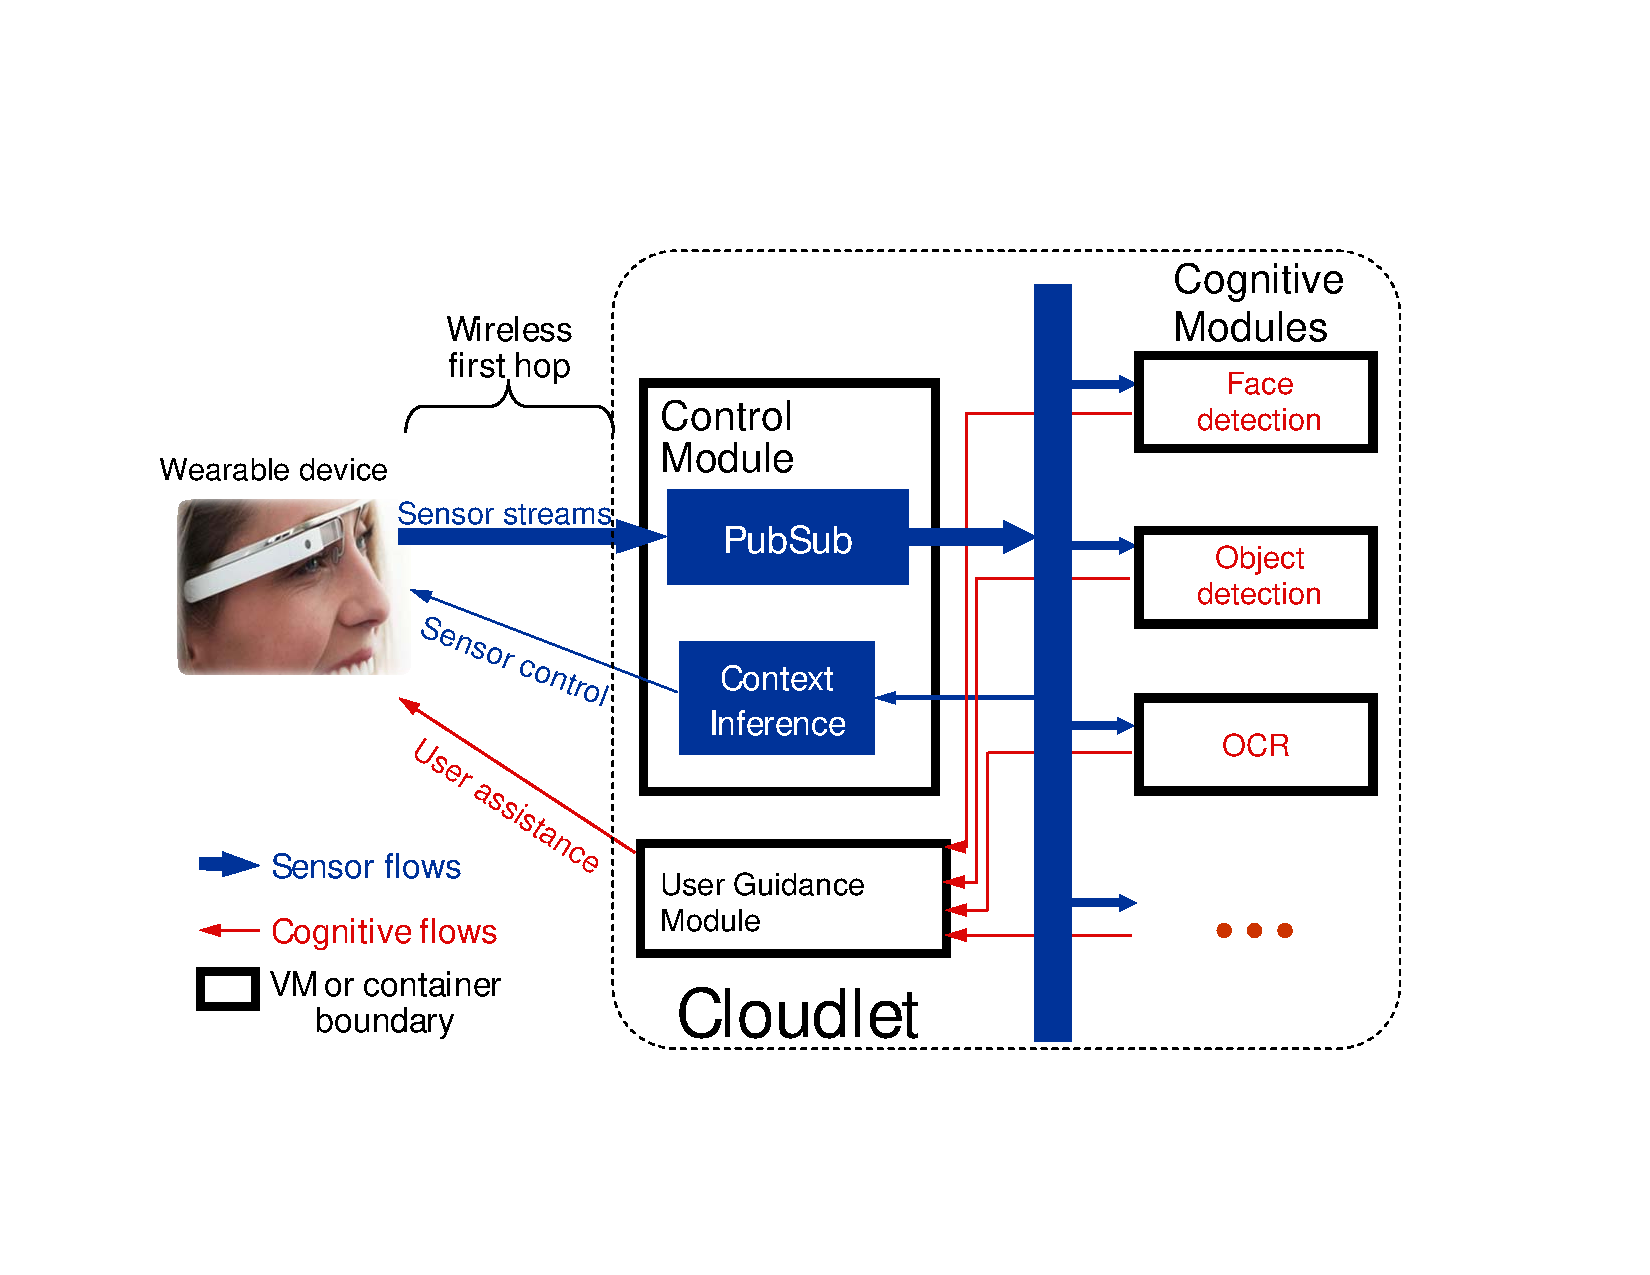
\includegraphics[width=0.8\linewidth]{FIGS/fig-backend-structure-simple-crop.pdf}
\begin{captiontext}
{\rm (Source: Chen et al~\cite{chen2017empirical})}
\end{captiontext}
\caption{\small Gabriel Platform}
\label{fig:gabriel}
\end{figure}

The Gabriel platform~\cite{ha2014towards,chen2017empirical}, shown in
Figure~\ref{fig:gabriel}, is the first application framework for wearable
cognitive assistance. It consists of a front-end running on wearable devices and
a back-end running on cloudlets. The Gabriel front-end performs preprocessing of
sensor data (e.g., compression and encoding), which it then streams over a
wireless network to a cloudlet.  The Gabriel back-end on the cloudlet has a
modular structure. The {\em control module} is the focal point for all
interactions with the wearable device and can be thought as an agent for a
particular client on the cloudlet. A publish-subscribe (PubSub) mechanism
distributes the incoming sensor streams to multiple {\em cognitive modules}
(e.g., task-specific computer vision algorithms) for concurrent processing.
Cognitive module outputs are integrated by a task-specific {\em user guidance
module} that performs higher-level cognitive processing such as inferring task
state, detecting errors, and generating guidance in one or more modalities
(e.g., audio, video, text, etc.). The Gabriel platform automatically discovers
cognitive engines on the local network via a universal plug-and-play (UPnP)
protocol. The platform is designed to run on a small cluster of machines with
each modules capable of being separated or co-located with other modules via
process, container, or virtual machine virtualization. 

The original Gabriel platform was built with a single user in mind, and did not
have mechanisms to share cloudlet resources in a controlled manner.  It did,
however, have a token-based transmission mechanism.  This limited a client to
only a small number of outstanding operations, thereby offering a simple form of
rate adaptation to processing or network bottlenecks.  We have retained this
token mechanism in our system, described in the rest of this thesis. In
addition, we have extended Gabriel with new mechanisms to handle multi-tenancy,
perform resource allocation, and support application-aware adaptation.  We refer
to the two versions of the platform as ``Original Gabriel'' and ``Scalable
Gabriel.''

\section{Example Gabriel Applications}
\label{sec:example-apps}

Many applications have been built on top of the Gabriel platform.
Figure~\ref{fig:bg-apps-table} provides a summary of applications built by Chen
et al~\cite{chen2018application}. These applications run on multiple wearable
devices such as Google Glass, Microsoft HoloLens, Vuzix Glass, and ODG R7. At a
high level, the cloudlet workflows of these applications are similar, and
consist of two major phases. The first phase uses computer vision to extract a
symbolic, idealized representation of the state of the task, accounting for
real-world variations in lighting, viewpoint, etc.  The second phase operates on
the symbolic representation, implements the logic of the task at hand, and
occasionally generates guidance for the user.  In most WCA applications, the
first phase is far more compute intensive than the second phase. While visual
data is the focus of the analysis, other types of sensor data, e.g. audio, are
also used to help infer user state.

Leveraging lessons learned by Chen et al~\cite{chen2018application}, we created
and implemented several real-life WCA applications whose tasks are more complex.
They also pose more challenges to the computer vision processing as the parts
are not designed for machine recognition. In particular, we focused on assembly
tasks. Many assembly tasks, including manufacturing assembly and medical
procedures, are tedious and error-prone. WCAs can help reduce errors, provide
training, and assist human operators by continuously monitoring their actions and
offering feedback. We describe two of these applications below in detail.

\begin{figure}
\centering
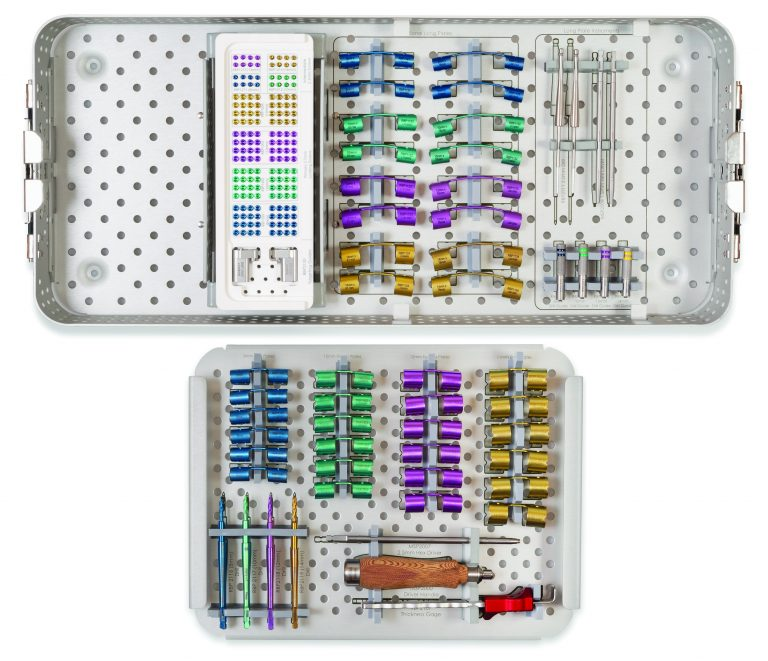
\includegraphics[width=0.5\linewidth]{FIGS/RibLoc.jpg}
\caption{\small RibLoc Kit}
\label{fig:ribloc}
\end{figure}

\begin{figure}
\centering
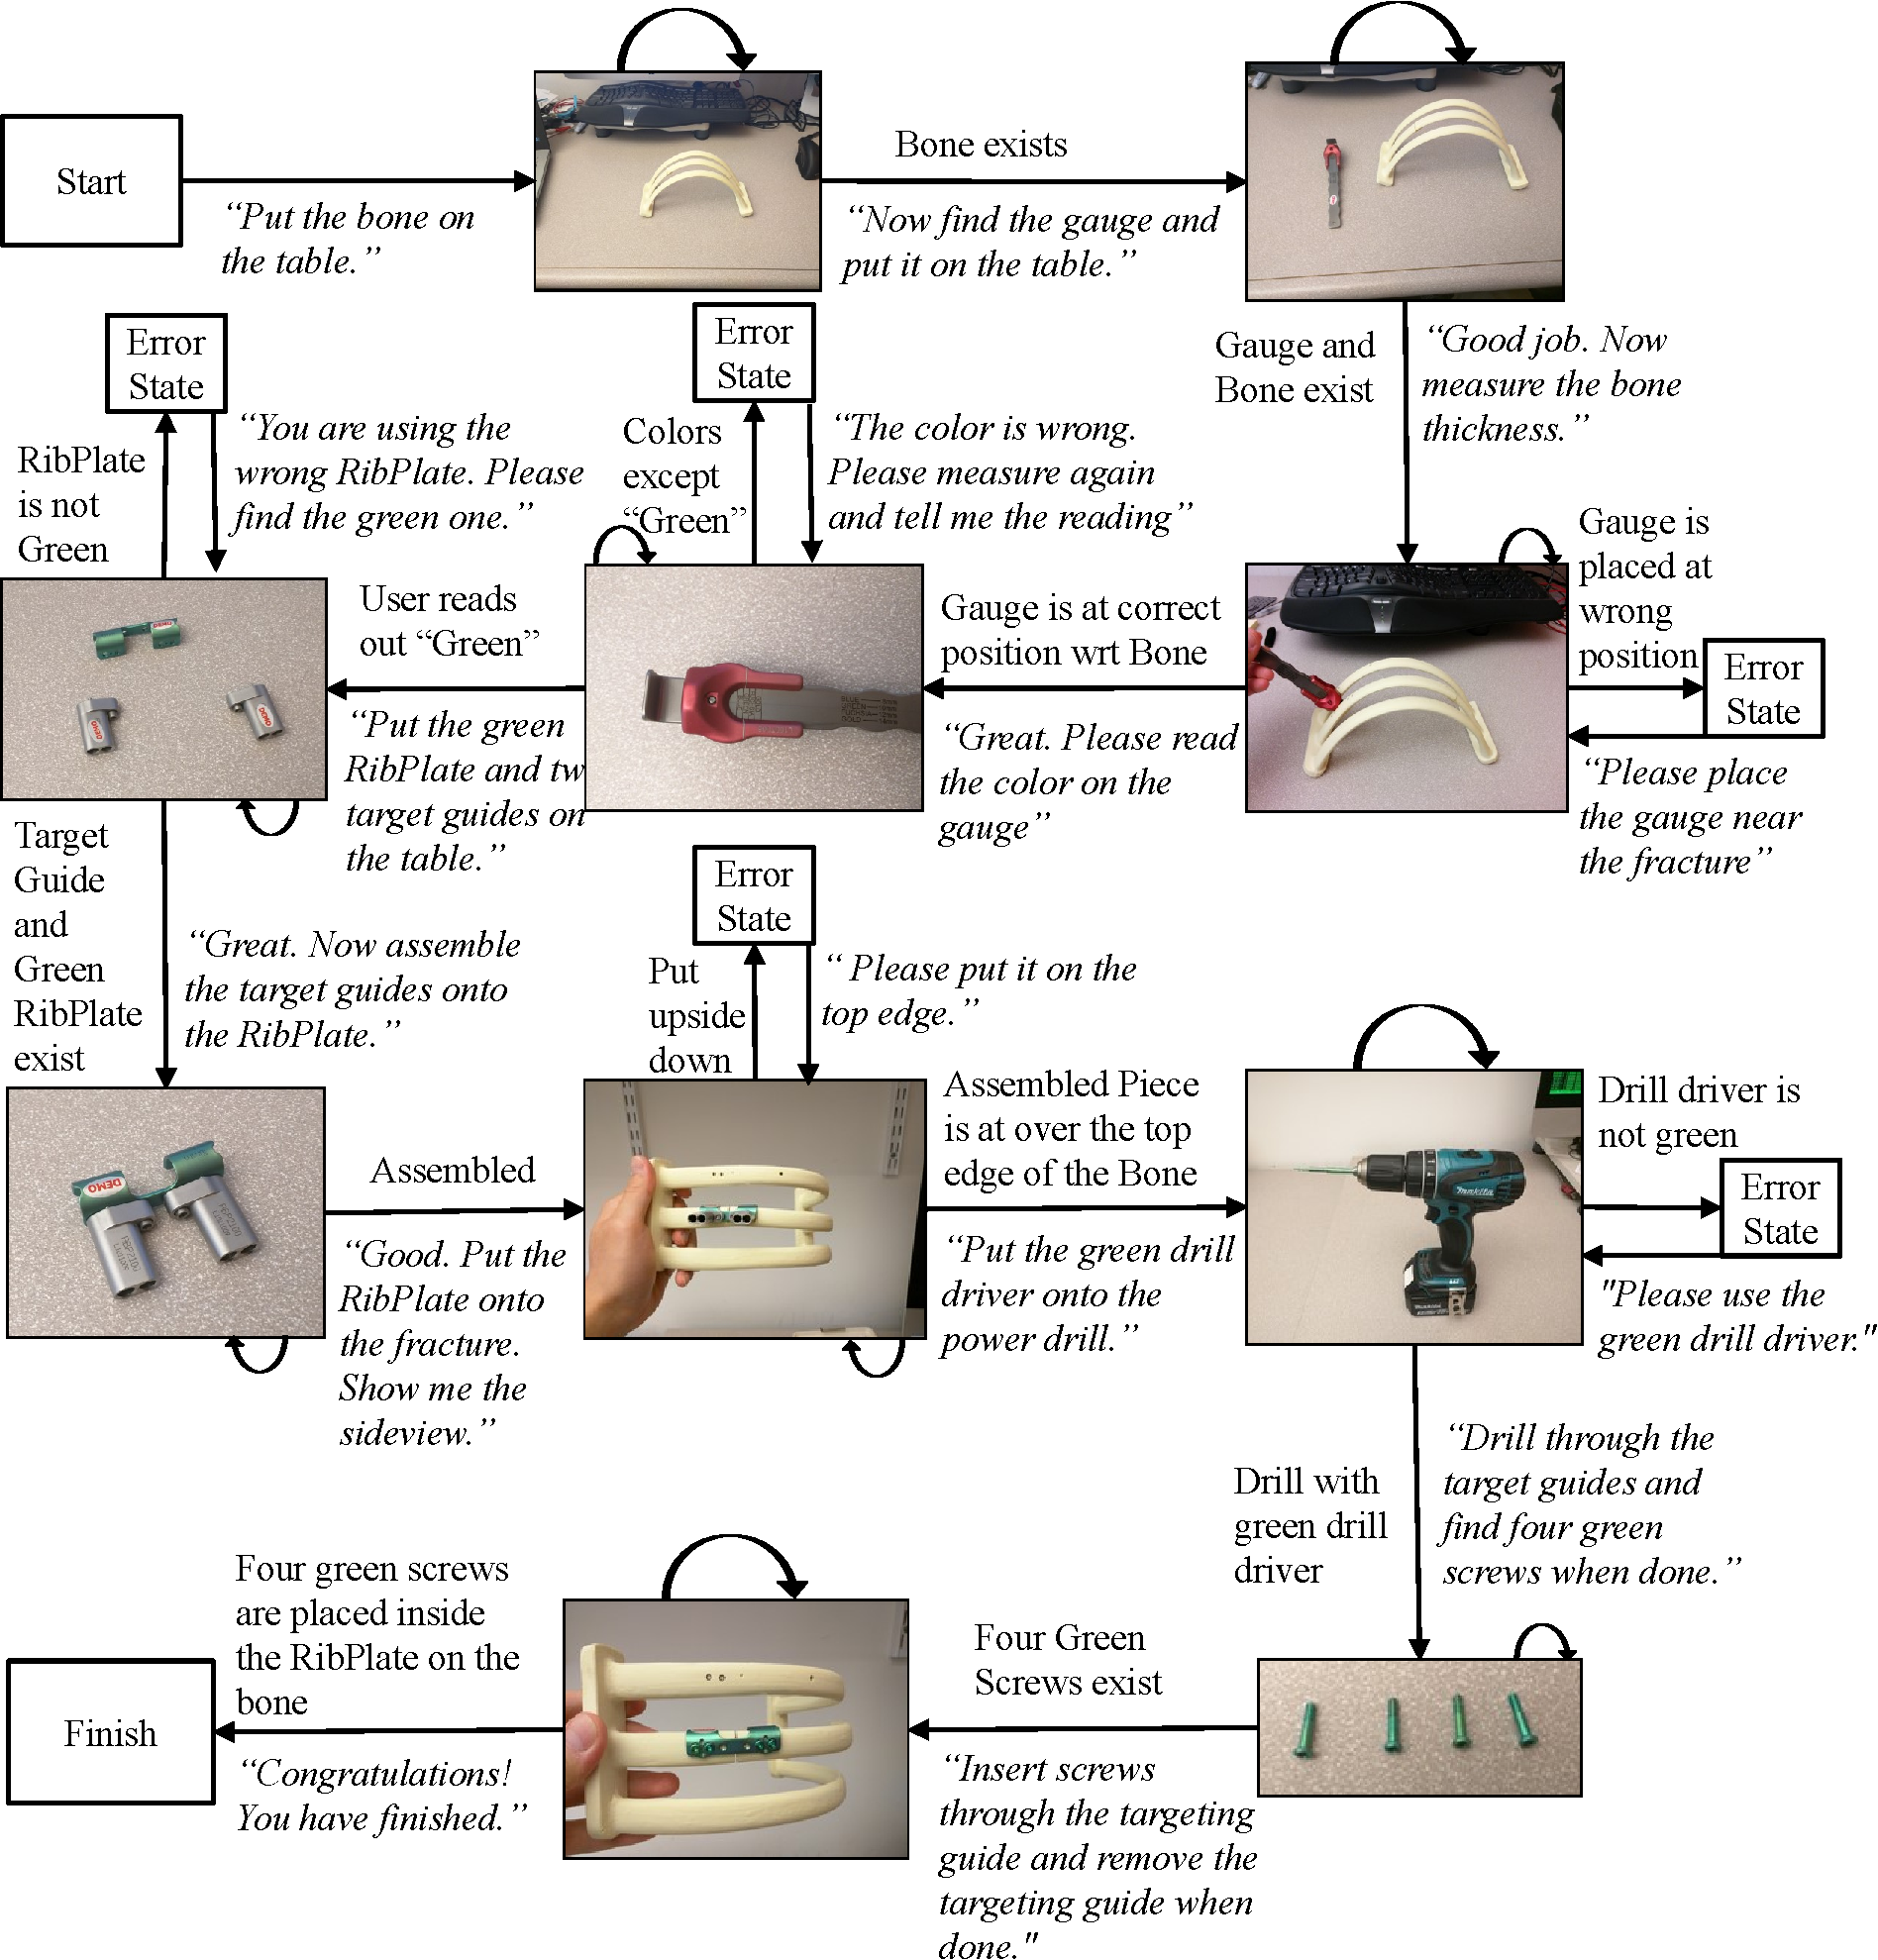
\includegraphics[width=\linewidth]{FIGS/ribloc-fsm-crop.pdf}
\caption{\small RibLoc Assistant Task State Machine}
\label{fig:ribloc-app}
\end{figure}

\subsection{RibLoc Application}

RibLoc Fracture Plating System~\cite{ribloc}, shown in Figure~\ref{fig:ribloc}
is used by surgeons to fixate broken ribs for fracture repair. They surgery
consists of five major steps: measure ribs thickness, prepare the plate, drill
bone for screw insertion, insert screws, and tighten screws. To train doctors
how to use this kit, Acute Innovations, the manufacturer of RibLoc, currently
send sales personnel to doctors' office, often for extended period of time. To
reduce the cost of training, we develop a WCA for RibLoc that guides a surgeon
to learn RibLoc step-by-step on fake bones. Figure~\ref{fig:ribloc-app} shows
the task steps of the application as a finite state machine (FSM). Conditions of
state transitions are shown above the transition arrows and instructions
given to users are quoted shown in italics.
Most of user
state recognition is achieved by verifying the existence and locations of key
objects. One exception is rib thickness measurement. The application asks the
user to read out some text from the gauge. Automatic speech recognition (ASR) is
used to detect the user's read-out. ASR is used because the text on the gauge
has a low contrast with the background that they are too hard to optical
character recognition (OCR). A demo video of RibLoc WCA is at
\url{https://youtu.be/YRTXUty2P1U}.

\subsection{DiskTray Application}

\begin{figure}
\centering
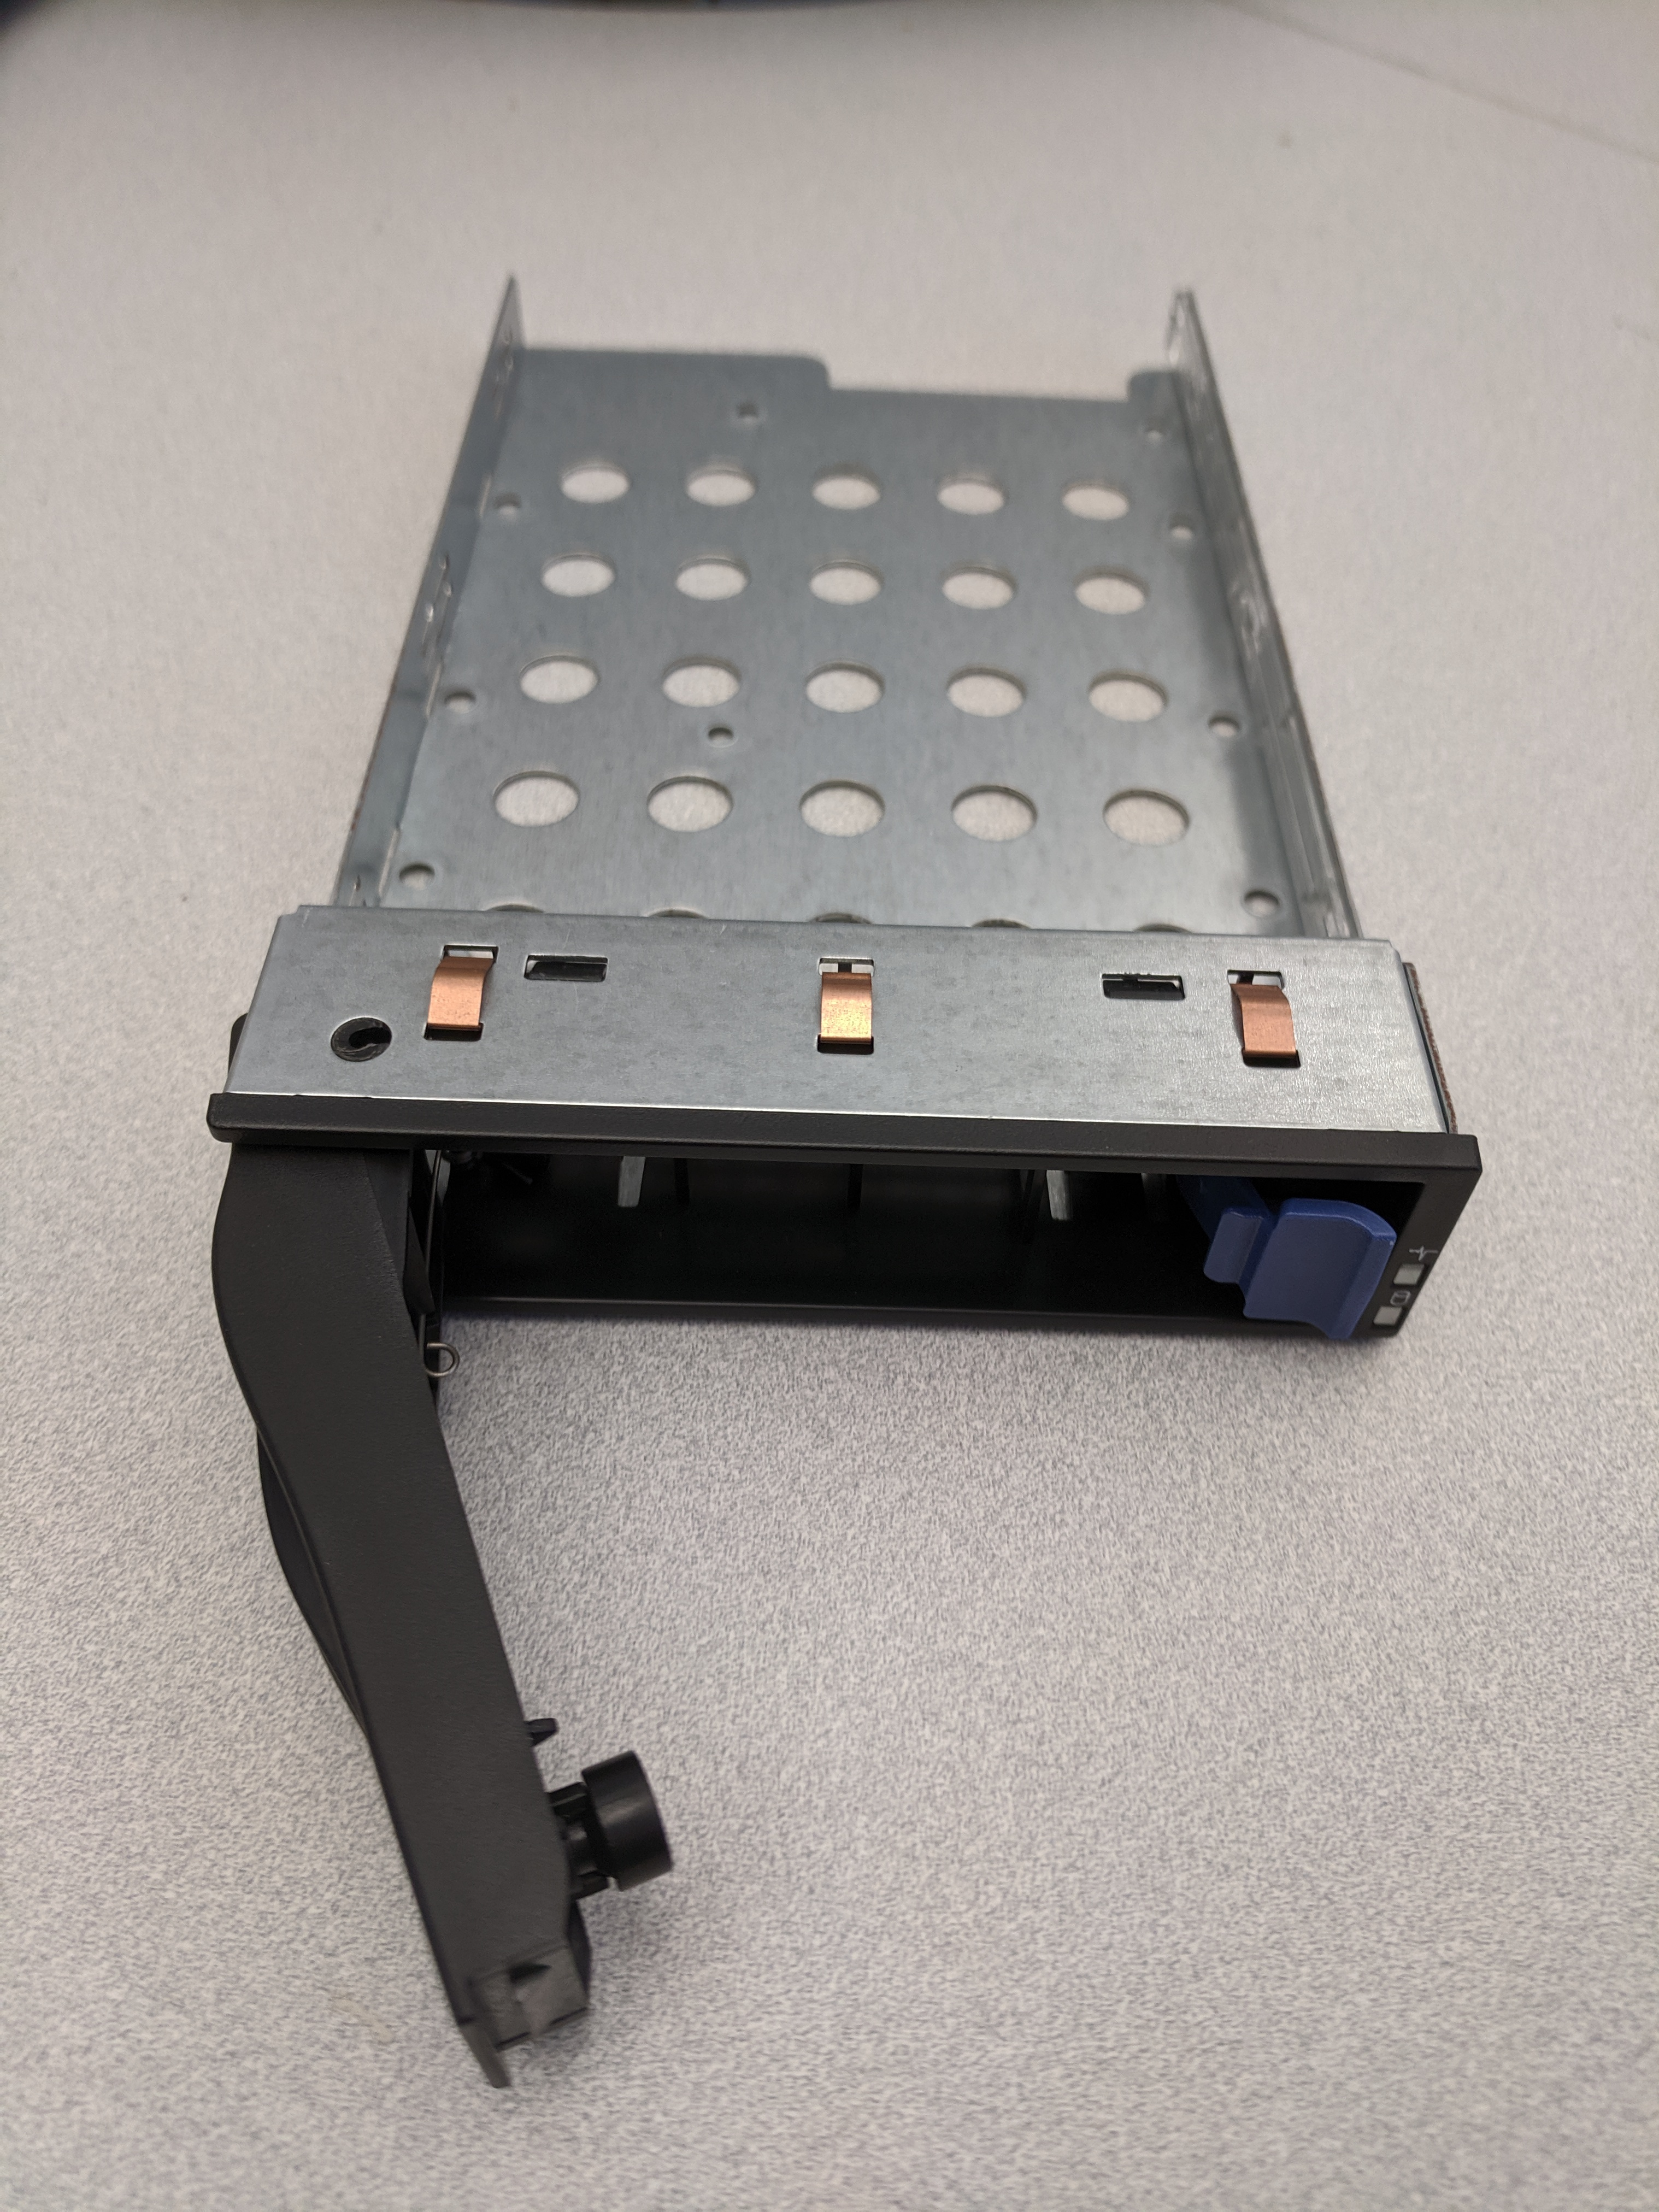
\includegraphics[width=0.3\linewidth]{FIGS/disktray.jpg}
\caption{\small Assembled DiskTray}
\label{fig:disktray}
\end{figure}

\begin{figure}
\centering
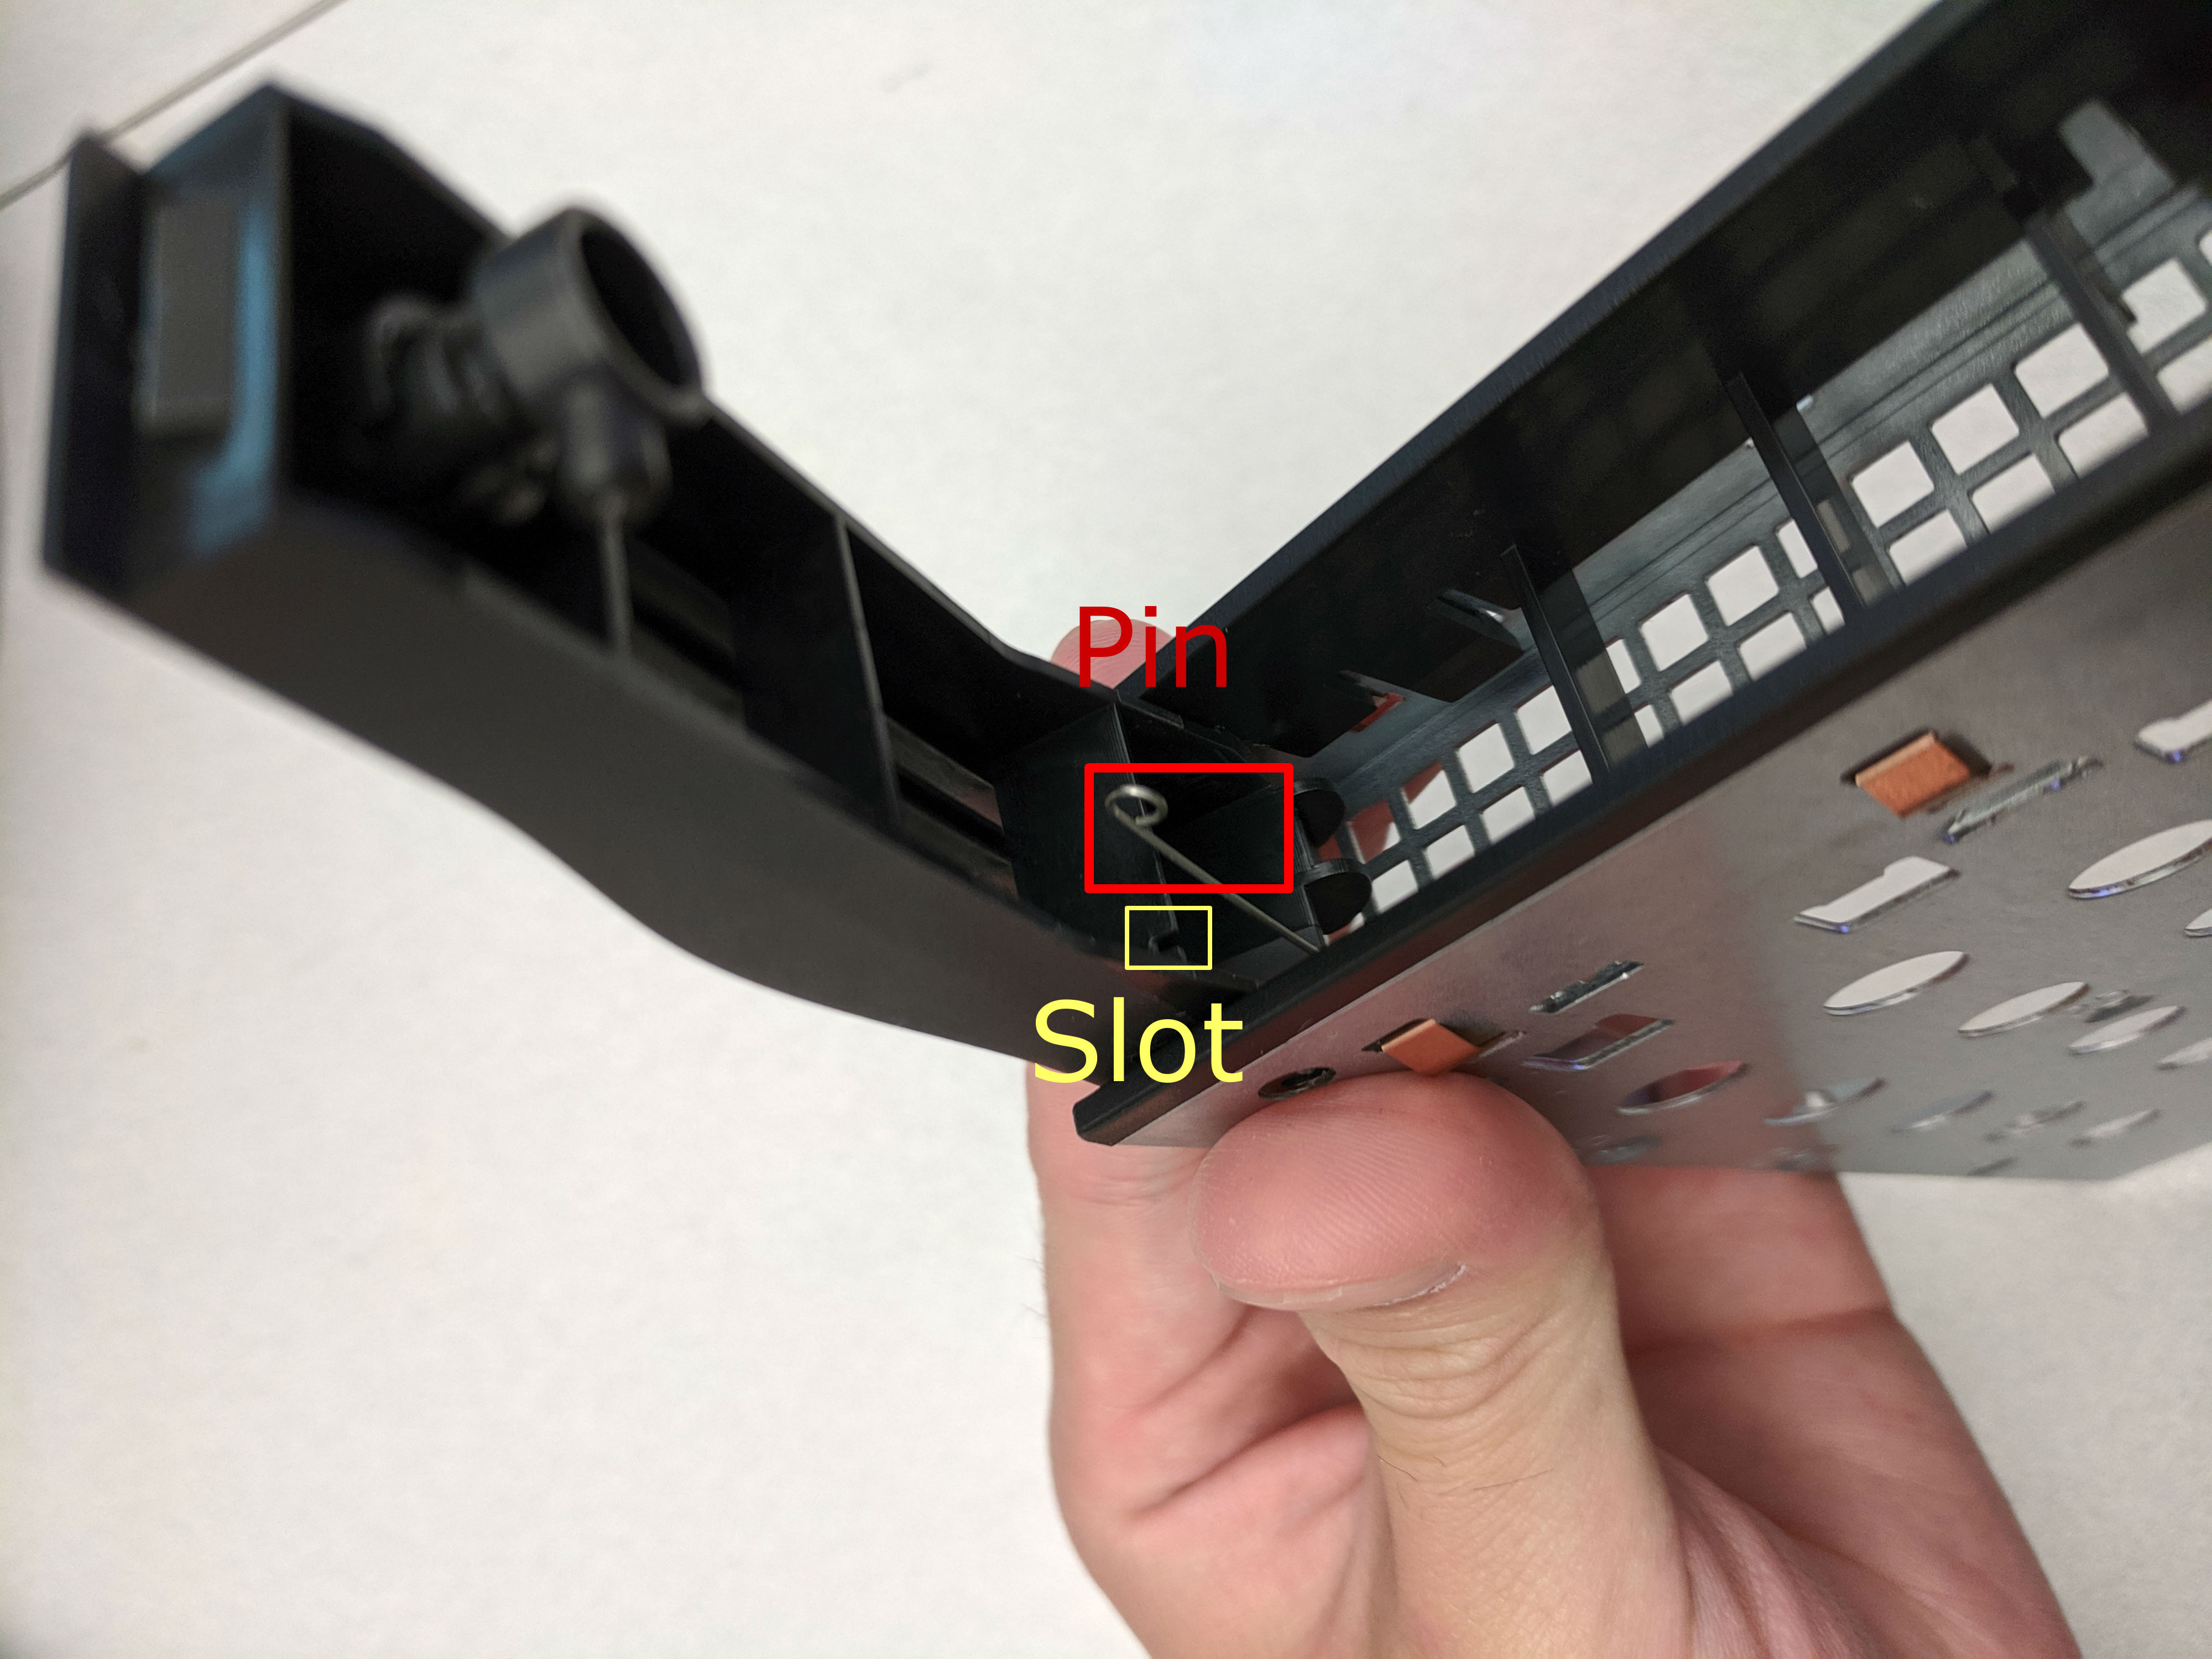
\includegraphics[width=0.5\linewidth]{FIGS/disktray-challenge.jpg}
\caption{\small Small Parts in DiskTray WCA}
\label{fig:disktray-challenge}
\end{figure}

In collaboration with InWin~\cite{inwin}, a computer hardware manufacturer, we
created a cognitive assistance to train operators how to assemble their disk
tray product. Figure~\ref{fig:disktray} shows the assembled tray, which is used
to host hard drives that go into a server chassis. As all the other WCAs, we do
not modify the original parts. 

We face two challenges when building this application. First, some parts are
tiny. In one step, the application needs to check if a pin is placed correctly
into a slot. As shown in Figure~\ref{fig:disktray-challenge}, both the slot and
the pin are tiny and hard to see. To facilitate the detection of these two
parts, we ask the user to bring the parts close to the camera in addition to
zooming the camera and turning on the camera flashlight. Second, there is a
plastic strip that is translucent. Transparent objects are extremely challenging
to detect using 2D RGB cameras, because their appearance depends on the
background and lighting~\cite{lysenkov2013recognition}. Instead of detecting the
placement of the transparent strip by computer vision, we leverage the human
operator to signal to the system when the operation is completed. InWin
showcased this application at 2018 Computex Technology Show~\cite{computex}. A
demo video of the Computex Demo can be viewed
at~\url{https://www.youtube.com/watch?v=AwWZcL9XGI0}.


\section{Application Latency Bounds}

\begin{figure}
\centering
\begin{tabular}{|l|c|c|c|c|c|c|c|}
\hline
                      & Pool & Work-out & Ping-pong & Face &
                      \multicolumn{3}{c|}{
                          \begin{tabular}{@{}c@{}}Assembly Tasks\\ (e.g. RibLoc)\end{tabular}} \\
\hline
\Xhline{2\arrayrulewidth}
\hline
    Bound Range (tight-loose) & 95-105 & 300-500 & 150-230 & 370-1000 & \multicolumn{3}{c|}{600-2700} \\
\hline
\end{tabular}
\caption{Application Latency Bounds (in milliseconds)}
\begin{captiontext}
{\rm (Adapted from Chen et al~\cite{chen2017empirical})}
\end{captiontext}
\label{fig:bg-bounds}
\end{figure}

Not only are the accuracy of the instructions important to WCAs, but the speed
at which these instructions are delivered is also critical. With a human in the
loop, the latency requirements of WCAs are closely related to the task-specific
human speed. For example, for assembly tasks, an instruction delivered tens of
seconds after a user has finished a step can cause user annoyance and
frustration. For PINGPONG assistant, a task that is even more fast-paced, an
instruction on where to hit the ball becomes useless if it is delivered after
the user has made a hit. 

Previous work~\cite{chen2017empirical} quantifies task-dependent application
latency bounds by answering the question \textit{How fast does an instruction
need to be delivered?} Three different approaches are used. For tasks that have
published human speed, numbers from the literature are used as the upper bound
of the end-to-end system response time. For example, it takes about 1000 ms for
a human to recognize the identity of a face. Therefore, a face recognition
assistant should deliver a person's name faster than 1000ms to exceed human
speed. For tasks in which users interact with physical systems, the latency
bounds can be derived directly from first principles of physics. For instance,
the latency bounds for PINGPONG assistant are calculated by subtracting audio
perception time, motion initiation time, and swinging time from the average time
between opponents hitting the ball. In addition, an user study of LEGO assembly
assistant is also conducted to deduct latency bounds for assembly tasks.

Figure~\ref{fig:bg-bounds} shows a summary of latency bounds calculated from the
previous work~\cite{chen2017empirical}. Each application is assigned both a
tight and a loose bound from the application perspective. The tight bound
represents an ideal target, below which the user is insensitive to improvements.
Above the loose bound, the user becomes aware of slowness, and user experience
and performance is significantly impacted. Latency improvements between the two
limits may be useful in reducing user fatigue.

These application latency bounds can be considered as application quality of
service (QoS) metrics. Similar to bitrate and startup time in video streaming,
these metrics serve as measurable proxies to user experience. When the system
delay increases, we can compare the delay with these latency bounds to estimate
how much a user is suffering. In this thesis, we use these bounds to formulate
application utility functions, which quantify user experience when a system
response is delayed due to contention. These application utility functions are
the foundation for our adaptation-centered approach to scalability.


\begin{figure*}
\begin{tabular}{|p{0.31in}|p{0.95in}|p{3.5in}|p{0.84in}|p{0.8in}|}
\hline
App Name & Example Input Video Frame & Description & Symbolic \phantom{000} Representation & Example Guidance \\
\hline
\phantom{000} \textbf{Pool}     & \raisebox{-0.9\totalheight}{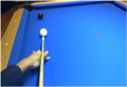
\psfig{file=FIGS/bigtable2/example-pool.png, width=0.97in}}
&
Helps a novice pool player aim correctly. Gives continuous visual feedback (left arrow, right arrow, or thumbs up) as the user turns his cue stick. Correct shot angle is calculated based on fractional aiming system~\cite{FractionalAiming}. Color, line, contour, and shape detection are used. The symbolic representation describes the positions of the balls, target pocket, and the top and bottom of cue stick.
&
\phantom{000} $<$Pocket, object ball, cue ball, cue top, cue bottom$>$ & \phantom{000} \raisebox{-0.85\totalheight}{
\psfig{file=FIGS/bigtable2/guidance-pool.png, width=0.8in}} \\
\hline
\phantom{000} \textbf{Ping-pong} & \raisebox{-0.9\totalheight}{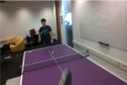
\psfig{file=FIGS/bigtable2/example-pingpong.png, width=0.97in}}
&
Tells novice to hit ball to the left or right, depending on which is more likely to beat opponent. Uses color, line and optical-flow based motion detection to detect ball, table, and opponent. The symbolic representation is a 3-tuple: in rally or not, opponent position, ball position. Whispers ``left'' or ``right'' or offers spatial audio guidance using~\cite{tang2014assistive}.

    Video URL: {\em \href{https://youtu.be/\_lp32sowyUA}{https://youtu.be/\_lp32sowyUA}}
&
\phantom{000} $<$InRally, ball position, opponent position$>$ & \phantom{000} Whispers ``Left!'' \\
\hline
\phantom{000} \textbf{Work-out} & \raisebox{-0.9\totalheight}{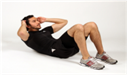
\psfig{file=FIGS/bigtable2/example-workout.png, width=0.97in}}
&
Guides correct user form in exercise actions like sit-ups and push-ups, and counts out repetitions. Uses Volumetric Template Matching~\cite{ke2007event} on a 10-15 frame video segment to classify the exercise.
%A poorly-performed repetition is classified as a distinct type of exercise (e.g. ``good pushup'' versus ``bad pushup'').
Uses smart phone on the floor for third-person viewpoint.
&
\phantom{000} $<$Action, count$>$ & \phantom{000} Says ``8 '' \\
\hline
\phantom{000} \textbf{Face}     & \raisebox{-0.9\totalheight}{
\psfig{file=FIGS/bigtable2/example-face.png, width=0.97in}}
&
Jogs your memory on a familiar face whose name you cannot recall. Detects and extracts a tightly-cropped image of each face, and then applies a state-of-art face recognizer using deep residual network~\cite{he2016deep}. Whispers the name of a person.
Can be used in combination with Expression~\cite{anam2014expression} to offer conversational hints.
&
\phantom{000} ASCII text of name & \phantom{000} Whispers ``Barack Obama'' \\
\hline
\phantom{000} \textbf{Lego} & \raisebox{-0.9\totalheight}{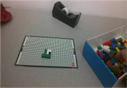
\psfig{file=FIGS/bigtable2/example-lego.png, width=0.97in}}
&
Guides a user in assembling 2D Lego models. Each video frame is analyzed in three steps: (i) finding the board using its distinctive color and black dot pattern; (ii) locating the Lego bricks on the board using edge and color detection; (iii) assigning brick color using weighted majority voting within each block. Color normalization is needed. The symbolic representation is a matrix representing color for each brick.

    Video URL: {\em \href{https://youtu.be/7L9U-n29abg}{https://youtu.be/7L9U-n29abg}}
&
\phantom{000} [[0, 2, 1, 1], \break [0, 2, 1, 6], \break [2, 2, 2, 2]] \break & \raisebox{-0.85\totalheight}{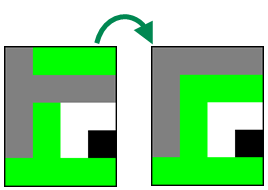
\psfig{file=FIGS/bigtable2/guidance-lego.png, width=0.8in}} Says ``Put a 1x3 green piece on top'' \\
\hline
\phantom{000} \textbf{Draw} & \raisebox{-0.9\totalheight}{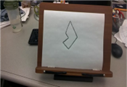
\psfig{file=FIGS/bigtable2/example-draw.png, width=0.97in}}
&
Helps a user to sketch better. Builds on third-party app~\cite{Iarussi2013} that was originally designed to take input sketches from pen-tablets and to output feedback on a desktop screen. Our implementation preserves the back-end logic. A new Glass-based front-end allows a user to use any drawing surface and instrument. Displays the error alignment in sketch on Glass.

    Video URL: {\em \href{https://youtu.be/nuQpPtVJC6o}{https://youtu.be/nuQpPtVJC6o}}
&
\raisebox{-0.85\totalheight}{
\psfig{file=FIGS/bigtable2/symbolic-draw.png, width=0.7in}} & \raisebox{-0.85\totalheight}{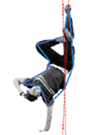
\psfig{file=FIGS/bigtable2/guidance-draw.png, width=0.8in}} \\
\hline
\phantom{000} \textbf{Sand-wich} & \raisebox{-0.9\totalheight}{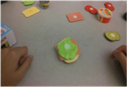
\psfig{file=FIGS/bigtable2/example-sandwich.png, width=0.97in}}
&
Helps a cooking novice prepare sandwiches according to a recipe. Since real food is perishable, we use a food toy with plastic ingredients. Object detection follows the state-of-art faster-RCNN deep neural net approach~\cite{ren2015faster}. Implementation is on top of Caffe~\cite{jia2014caffe} and Dlib~\cite{dlib09}. Transfer learning~\cite{Pan2010} helped us save time in labeling data and in training.

    Video URL: {\em \href{https://youtu.be/USakPP45WvM}{https://youtu.be/USakPP45WvM}}
&
\phantom{000} Object: \break ``E.g. Lettuce on top of ham and bread'' & \raisebox{-0.9\totalheight}{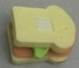
\psfig{file=FIGS/bigtable2/guidance-sandwich.jpg, width=0.7in}} Says ``Put a piece of bread on the lettuce'' \\
\hline

\end{tabular}
\caption{Prototype Wearable Cognitive Assistance Applications}
\label{fig:bg-apps-table}
\end{figure*}
\chapter{Application-Agnostic Techniques to Reduce Network Transmission}
\section{{\xc EarlyDiscard} S\lc{trategy}}
\label{sec:earlydiscard}

\subsection{Description}
EarlyDiscard is based on the idea of using on-board processing to filter and
transmit only interesting frames in order to save bandwidth when offloading
computation. Previous work~\cite{Hu2015}~\cite{Naderiparizi2017} leveraged
pixel-level features and multiple sensing modalities to select interesting
frames from hand-held or body-worn cameras. In this work, we explore the use
of DNNs to filter frames from aerial views. The benefits of using DNNs are
twofold. First, DNNs are trained and specialized for each task, resulting in
their high accuracy and robustness. Second, no additional hardware is added to
existing drone platforms.

Although smartphone-class hardware is incapable of supporting the
most accurate object detection algorithms at full frame rate today, it is
typically powerful enough to support less accurate algorithms.  These {\em weak
detectors} are typically designed for mobile platforms or were the state of the
art just a few years ago.  In addition, they can be biased towards high recall
with only modest loss of precision.  In other words, many clearly irrelevant
frames can be discarded by a weak detector, without unacceptably increasing the
number of relevant frames that are erroneously discarded.  This asymmetry is the
basis of the early discard strategy.

As shown in Figure~\ref{fig:ondrone}, we envision a choice of weak detectors
being available as early discard filters on a drone, with the specific choice of
filter being mission-specific.  Relative to the measurements presented in
Figure~\ref{fig:onboard-dnn-speed}, early discard only requires image
classification: it is not necessary to know exactly where in the frame a
relevant object occurs.  This suggests that MobileNet would be a good choice as
a weak detector. Its speed of 13 ms per frame on Jetson yields more than 75 fps.
We therefore use MobileNet on the drone for early discard in our experiments.

Pre-trained classifiers for MobileNet are available today for objects such as
cars, animals, human faces, human bodies, watercraft, and so on.  However, these
DNN classifiers have typically been trained on images that were captured from a
human perspective --- often by a camera held or worn by a person.  A drone,
however, has an aerial viewpoint and objects look rather different.  To improve
classification accuracy on drones, we used {\em transfer learning}~\cite{Yosinski2014} to finetune
the pre-trained classifiers on small training sets of images that were captured
from an aerial viewpoint.  This involves initial re-training of the last DNN
layer, followed by re-training of the entire network until convergence. Transfer
learning enables accuracy to be improved significantly for aerial images without
incurring the full cost of creating a large training set captured from an aerial
viewpoint.

Drone images are typically captured from a significant height, and hence objects
in such an image are small.  This interacts negatively with the design of many
DNNs, which first transform an input image to a fixed low resolution --- for
example, 224x224 pixels in MobileNet. Many important but small objects in the
original image become less recognizable.  It has been shown that small object
size correlates with poor accuracy in DNNs~\cite{Huang2017}.  To address this
problem, we {\em tile} high resolution frames into multiple sub-frames and then
perform recognition on the sub-frames.  This is done offline for training, as
shown in Figure~\ref{fig:tiling}, and also for online inference on the drone and
on the cloudlet.  The lowering of resolution of a sub-frame by a DNN is less
harmful, since the scaling factor is smaller.  Objects are represented by many
more pixels in a transformed sub-frame than if the entire frame had been
transformed.  The price paid for tiling is increased computational demand.  For
example, tiling a frame into four sub-frames results in four times the
classification workload.

\begin{figure}
  \hspace{-0.1in}
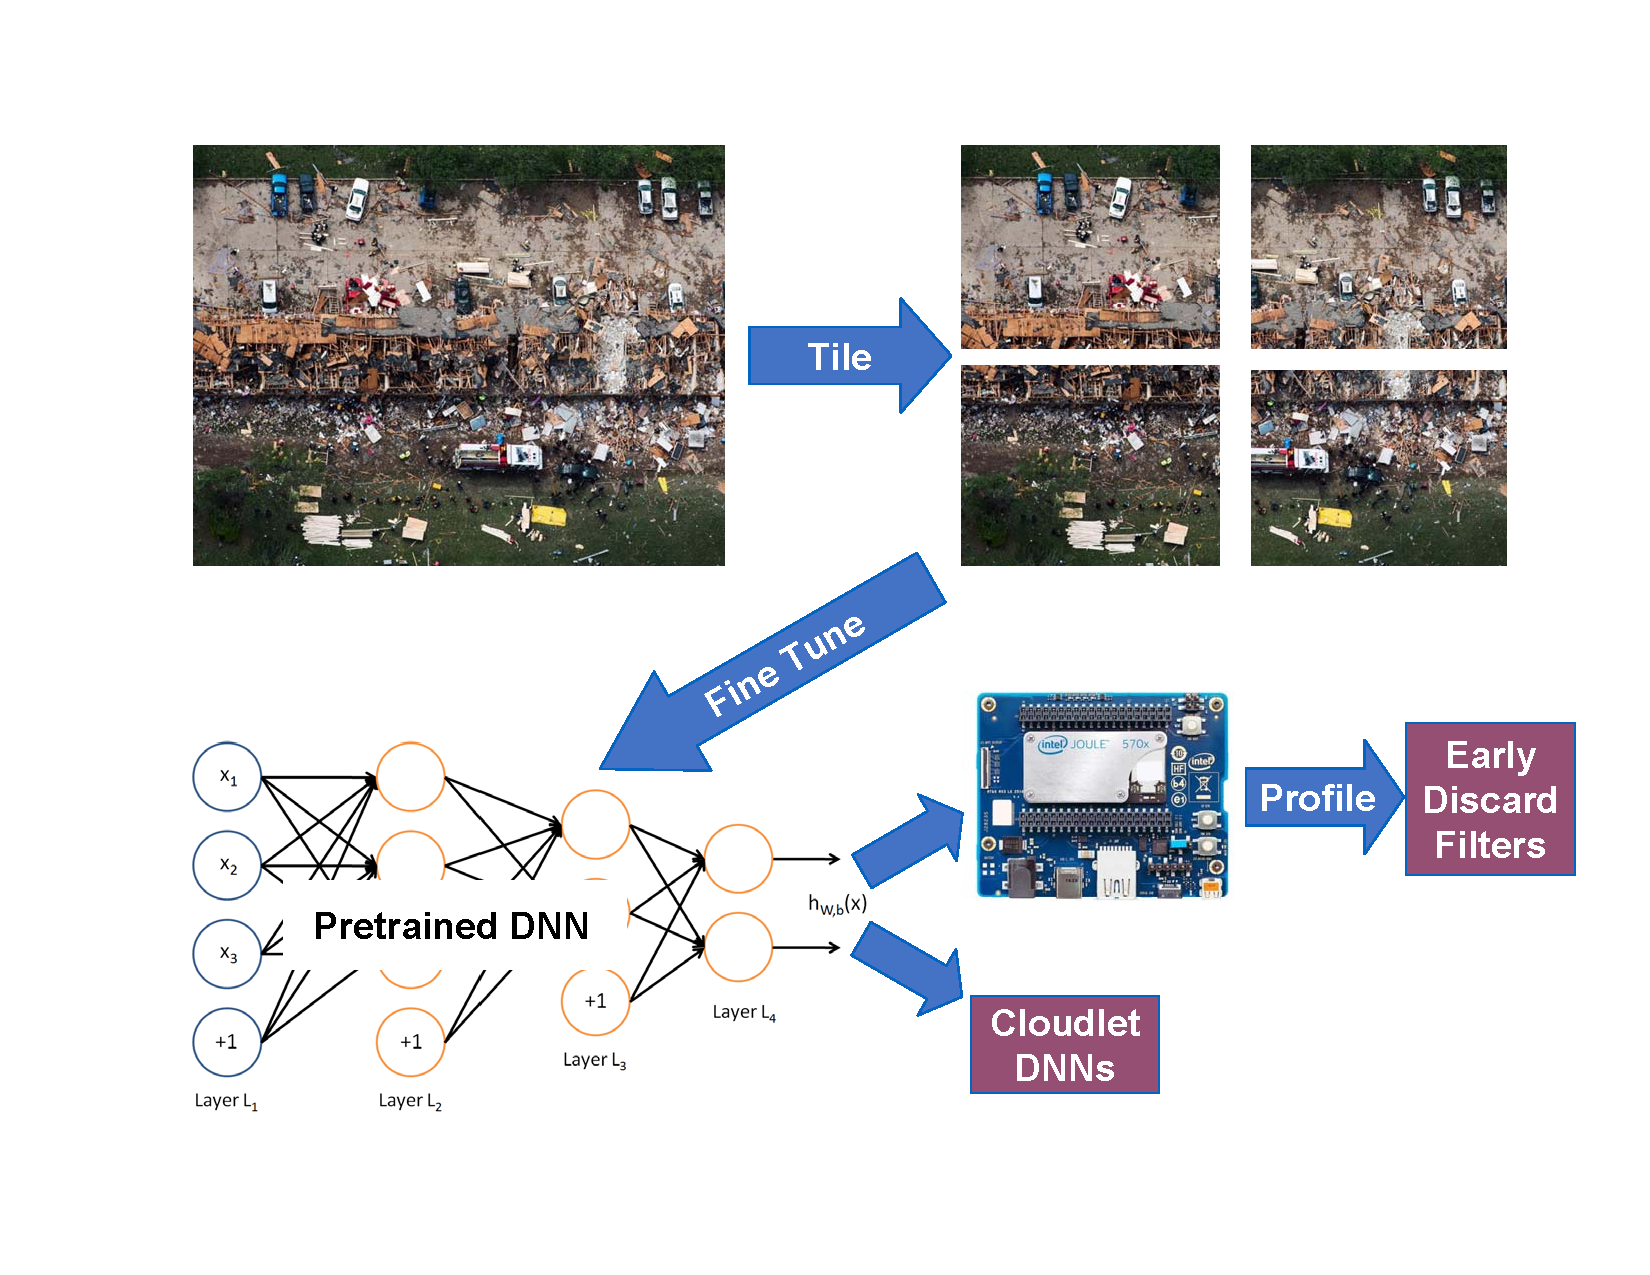
\psfig{file=FIGS/fig-training.pdf, scale=0.35}\\
\caption{Tiling and DNN Fine Tuning}
\label{fig:tiling}
\end{figure}

\subsection{Experimental Setup}

Our experiments on the {\xc EarlyDiscard}
strategy used the same benchmark suite described in
Section~\ref{sec:dumbdrone-setup}. We used Jetson TX2 as the drone platform. We use
both frame-based and event-based metrics to evaluate the MobileNet filters.

\subsection{Results of Early Discard Filters}
\label{sec:earlydiscard-result}

EarlyDiscard is able to significantly reduce the bandwidth consumed while
maintaining high result accuracy and low average delay. For three out of four
tasks, the average bandwidth is reduced by a factor of ten. Below we present
our results in detail.

\begin{figure}
\centering
\hspace*{-0.3in}
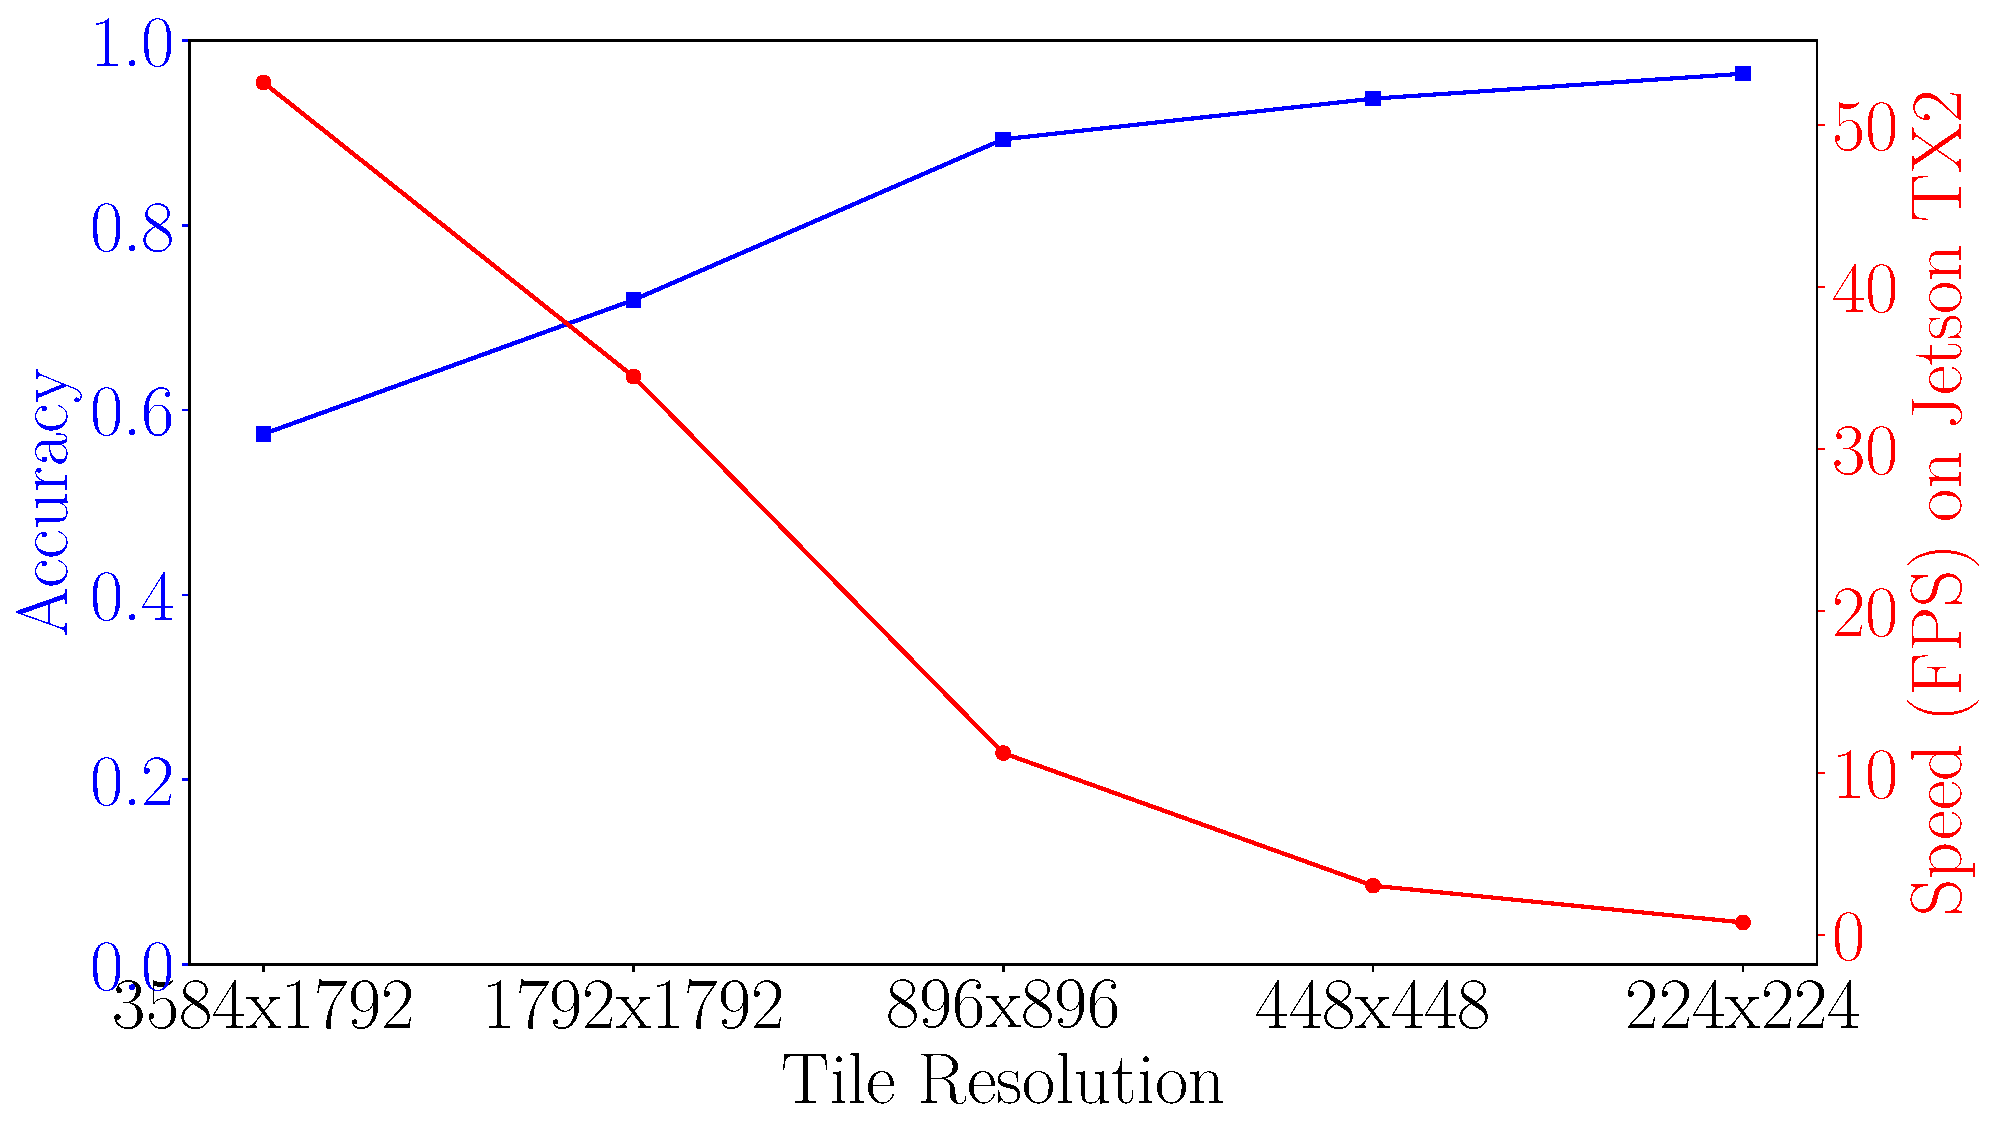
\psfig{file=FIGS/fig-tile-resolution-speed-accuracy.pdf, scale=0.2}
\caption{Speed-Accuracy Trade-off of Tiling}
\label{fig:earlydiscard-tile-accuracy-speed}
\vspace{-0.1in}
\end{figure}


\noindent{\textbf{Effects of Tiling}}: Tiling is used to improve the accuracy
for high resolution aerial images. We used the Okutama Action Dataset, whose
attributes are shown in row T1 of Figure~\ref{fig:benchmarksuite}, to explore
the effects of tiling.  For this dataset,
Figure~\ref{fig:earlydiscard-tile-accuracy-speed} shows how speed and accuracy
change with tile size.  Accuracy improves as tiles become smaller, but the
sustainable frame rate drops.  We group all tiles from the same frame in a
single batch to leverage parallelism, so the processing does not change linearly
with the number of tiles. The choice of an operating point will need to strike a
balance between the speed and accuracy.  In the rest of the paper, we use two
tiles per frame by default. 

\noindent{\textbf{Drone Filter Accuracy}}: The output of a drone filter is the
probability of the current tile being ``interesting.''  A tunable {\em cutoff
threshold} parameter specifies the threshold for transmission to the cloudlet.
All tiles, whether deemed interesting or not, are still stored in the drone
storage for post-mission processing.

Figure~\ref{fig:earlydiscard-frame-percent-breakdown} shows our results on all
four tasks. Events such as detection of a raft in T3 occur in consecutive
frames, all of which contain the object of interest. A correct detection of an
event is defined as at least one of the consecutive frames being transmitted to
the cloudlet.  Blue lines in
Figure~\ref{fig:earlydiscard-frame-percent-breakdown} shows how the event
recalls of drone filters for different tasks change as a function of cutoff
threshold. The MobileNet DNN filter we used is able to detect all the events for
T1 and T4 even at a high cutoff threshold. For T2 and T3, the majority of the
events are detected. Achieving high recall on T2 and T3 (on the order of 0.95 or
better) requires setting a low cutoff threshold.  This leads to the possibility
that many of the transmitted frames are actually uninteresting (i.e., false
positives).

%% \begin{figure}
%% \includegraphics[width=0.6\linewidth]{FIGS/fig-event-recall-vs-threshold.pdf}
%% \vspace{-0.1in}
%% \caption{Drone Filter Recall vs. Cutoff Threshold}
%% \label{fig:event-recall-vs-threshold}
%% \end{figure}


\noindent{\textbf{False negatives}}: As discussed earlier, false negatives are
a source of concern with early discard.  Once the drone drops a frame
containing an important event, improved cloudlet processing cannot help. The
results in the third column of Figure~\ref{fig:early-discard-results} confirm
that there are no false negatives for T1 and T4 at a cutoff threshold of 0.5.
For T2 and T3, lower cutoff thresholds are needed to achieve perfect recalls.

\begin{figure}
    \centering
    
\includegraphics[width=0.8\linewidth]{FIGS/fig-event-recall-frame-percentage-legend.pdf}
    \hspace*{-0.3in}
    \begin{subfigure}[T1]{
        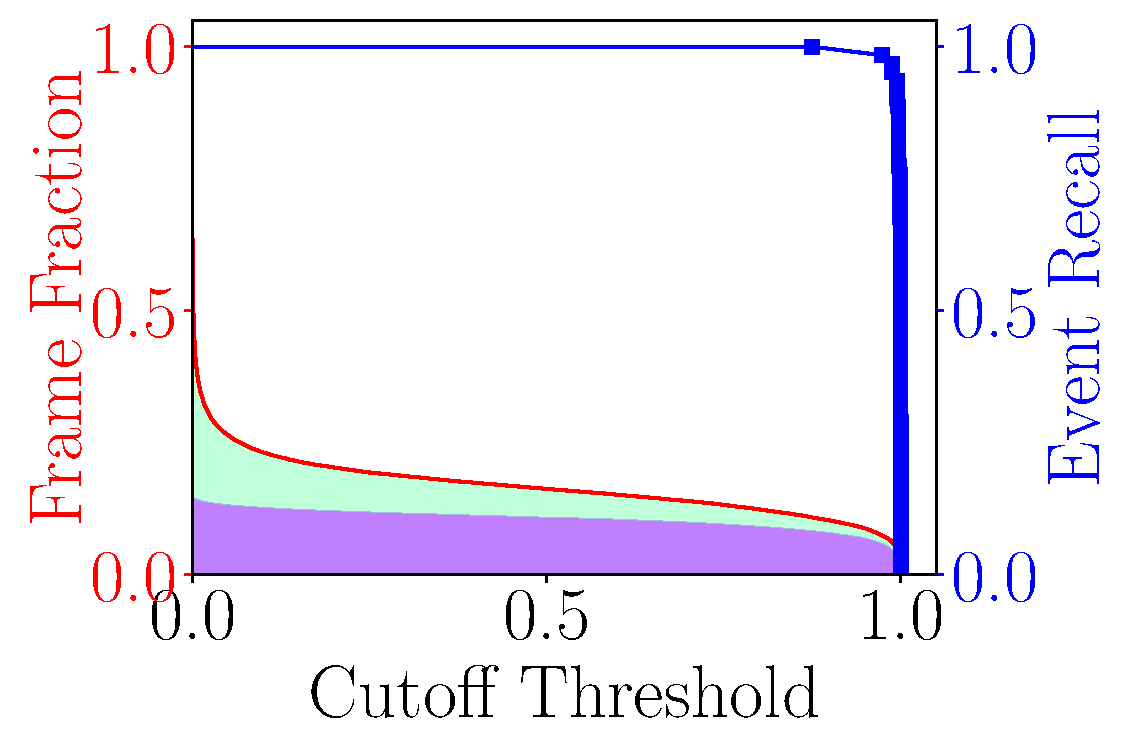
\includegraphics[width=0.5\linewidth]{FIGS/fig-event-recall-frame-percentage-vs-threshold-okutama.pdf}}        
    \end{subfigure}
    \begin{subfigure}[T2]{
      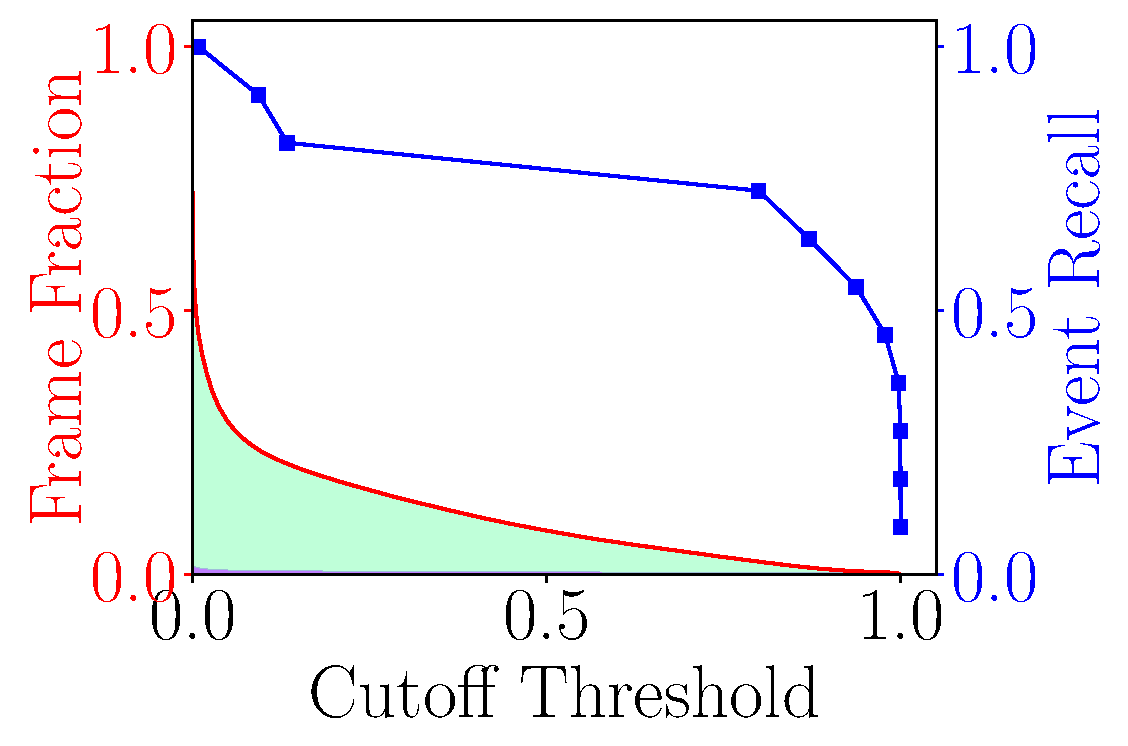
\includegraphics[width=0.5\linewidth]{FIGS/fig-event-recall-frame-percentage-vs-threshold-stanford.pdf}}
    \end{subfigure}
    \hspace*{-0.3in}    
    \begin{subfigure}[T3]{
      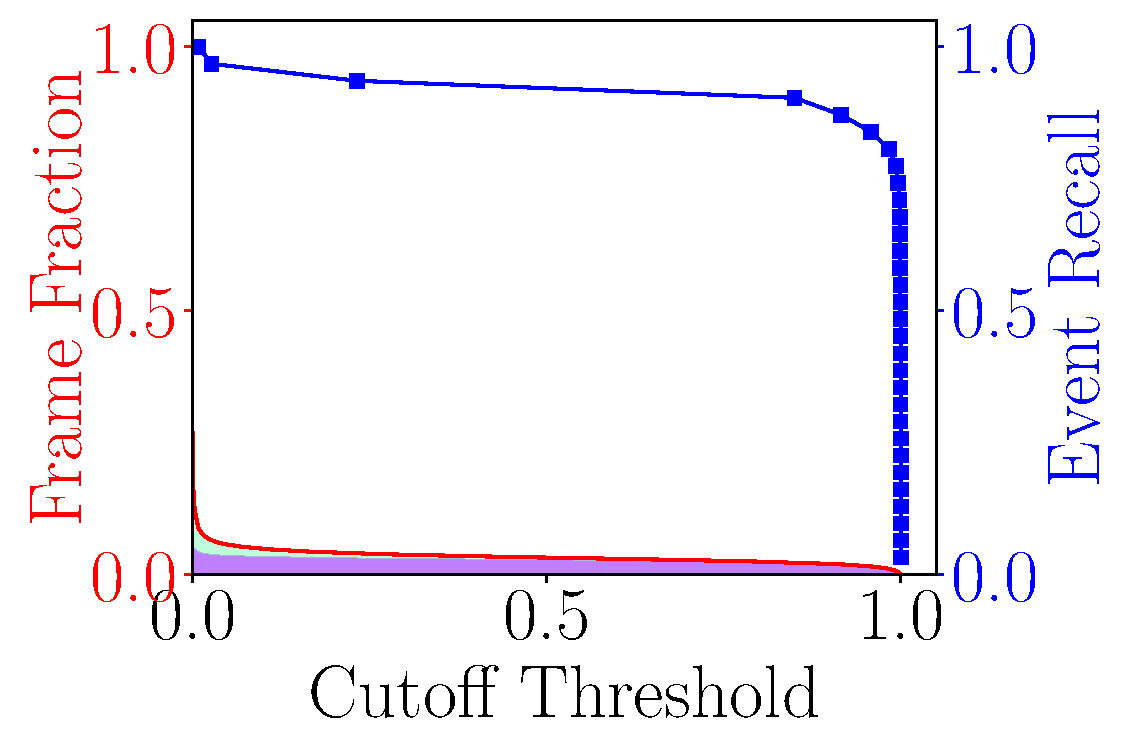
\includegraphics[width=0.5\linewidth]{FIGS/fig-event-recall-frame-percentage-vs-threshold-raft.pdf}}
    \end{subfigure}
    \begin{subfigure}[T4]{
      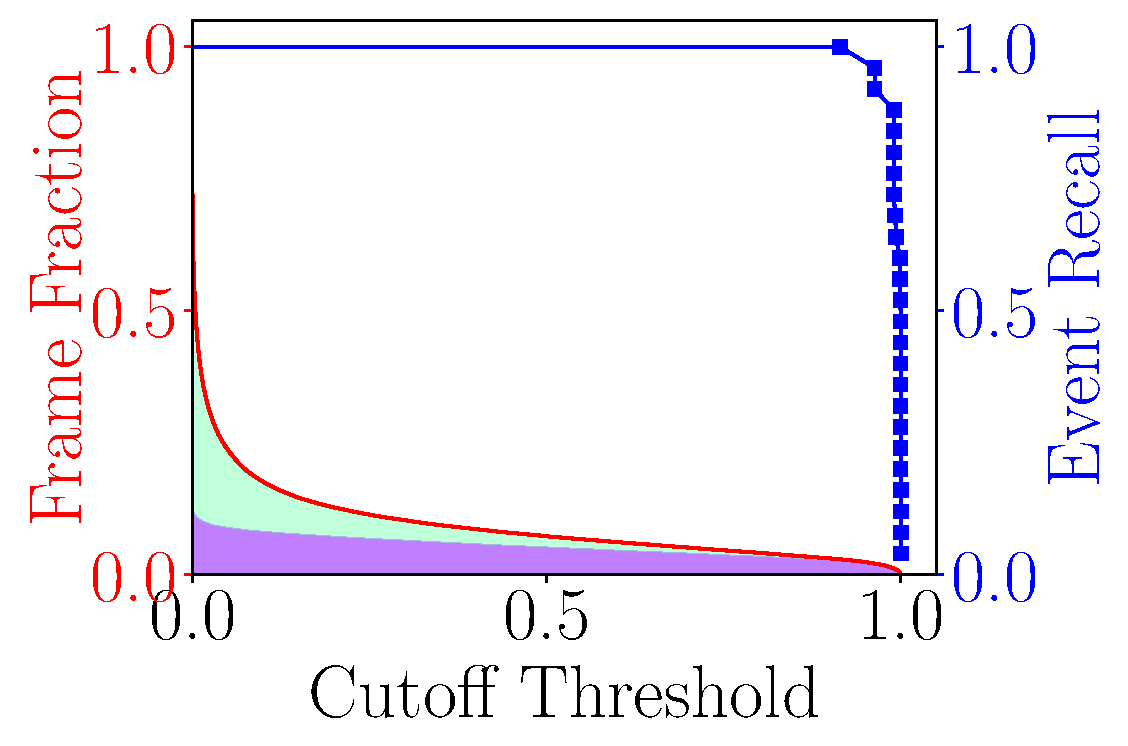
\includegraphics[width=0.5\linewidth]{FIGS/fig-event-recall-frame-percentage-vs-threshold-elephant.pdf}}
    \end{subfigure}
\caption{Where the Bandwidth Goes}
\label{fig:earlydiscard-frame-percent-breakdown}
\end{figure}

\begin{figure}
\hspace{-0.15in}
%\centering
\begin{tabular}{|c|c|c|c|c|c|c|}
\hline
   &Task   &Dete-       &Avg&Total&Avg&Peak\\
   &Total&cted&Delay&Data&B/W&B/W\\
   &Events&Events&(s)&(MB)&(Mbps)&(Mbps)\\ 

\hline
T1 & \phantom{0}62  & 100~\%       &  \phantom{0}0.1&\phantom{0}441  &  5.10     &   10.7  \\
\hline
T2 & \phantom{0}11  & \phantom{0}73~\%      & \phantom{0}4.9 & \phantom{00}13            &  0.03 & \phantom{0}7.0 \\ % 100% recall at 47% of frames, 82% recall at 21% of frames
\hline
T3 & \phantom{0}31  & \phantom{0}90~\%  & 12.7 & \phantom{00}93  &  0.24 &  \phantom{0}7.0 \\ % 100% recall at 9% frames
\hline
T4 & \phantom{0}25  & 100~\%       & \phantom{0}0.3 & \phantom{0}167  &  0.43 &  \phantom{0}7.0 \\
\hline
\end{tabular}\\
\caption{Recall, Event Latency and Bandwidth at Cutoff Threshold 0.5}
\label{fig:early-discard-results}
\end{figure}

\noindent{\textbf{Result latency}}:
The contribution of early discard processing to total result latency
is calculated as the average time difference between the first frame
in which an object occurs (i.e., first occurrence in ground truth) and
the first frame containing the object that is transmitted to the
backend (i.e., first detection).  The results in the fourth column of
Figure~\ref{fig:early-discard-results} confirm that early discard
contributes little to result latency.  The amounts range from 0.1~s
for T1 to 12.7~s for T3.  At the timescale of human actions
such as dispatching of a rescue team, these are negligible delays.

\noindent{\textbf{Bandwidth}}: Columns 5--7 of
Figure~\ref{fig:early-discard-results} pertain to wireless bandwidth demand for
the benchmark suite with early discard.  The figures shown are based on H.264
encoding of each individual frames in the drone-cloudlet video transmission.
Average bandwidth is calculated as the total data transmitted divided by
mission duration.  Comparing column 5 of Figure~\ref{fig:early-discard-results}
with column 2 of Figure~\ref{fig:baseline}, we see that all videos in the
benchmark suite are benefited by early discard (Note T3 and T4 have the same
test dataset as T2). For T2, T3, and T4, the bandwidth is reduced by more than
10x. The amount of benefit is greatest for rare events (T2 and T3).  When
events are rare, the drone can drop many frames.

Figure~\ref{fig:earlydiscard-frame-percent-breakdown} provides deeper insight
into the effectiveness of cutoff-threshold on event recall. It also shows how
many true positives (violet) and false positives (aqua) are
transmitted. Ideally, the aqua section should be zero.  However for T2, most
frames transmitted are false positives, indicating the early discard filter has
low precision.  The other tasks exhibit far fewer false positives.  This
suggests that the opportunity exists for significant bandwidth savings if
precision could be further improved, without hurting recall.


\subsection{Use of Sampling}

\begin{figure}
    \centering
    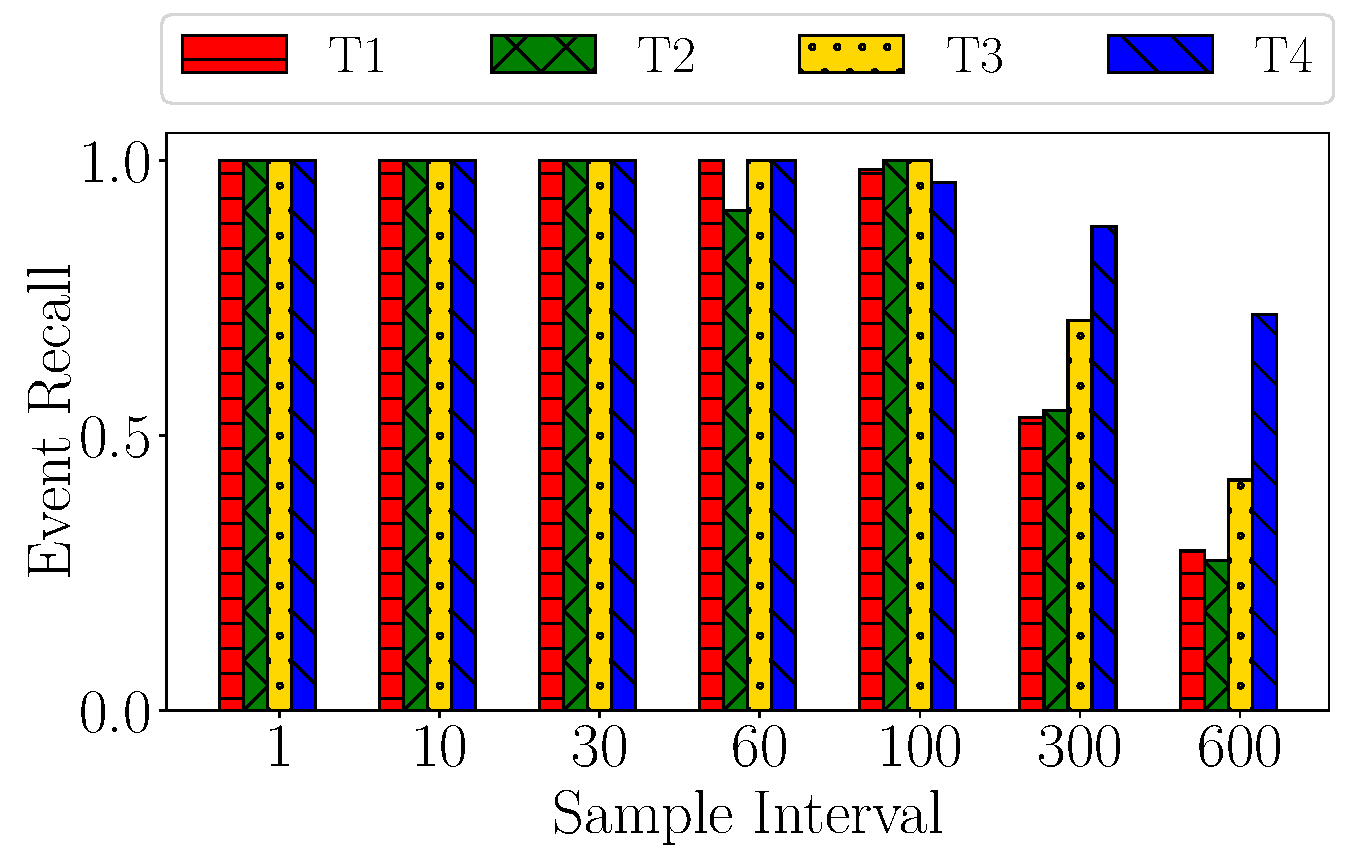
\includegraphics[width=\linewidth]{FIGS/fig-random-select-interval-recall-hatch.pdf}
\caption{Event Recall at Different Sampling Intervals}
\label{fig:sampling-only}
\end{figure}


  
\begin{figure}
    \centering
    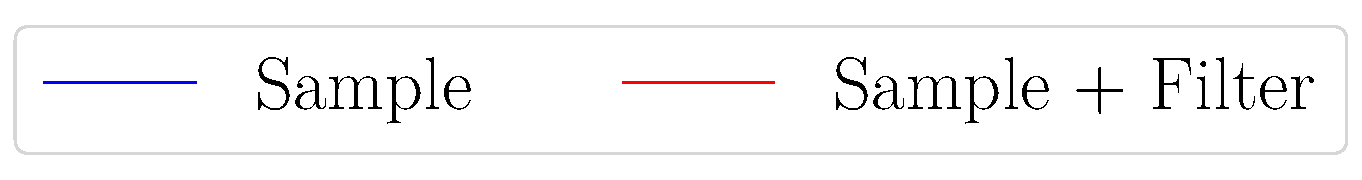
\includegraphics[width=0.7\linewidth]{FIGS/fig-recall-frame-aggregated-legend.pdf}
    \begin{subfigure}[T1]{
        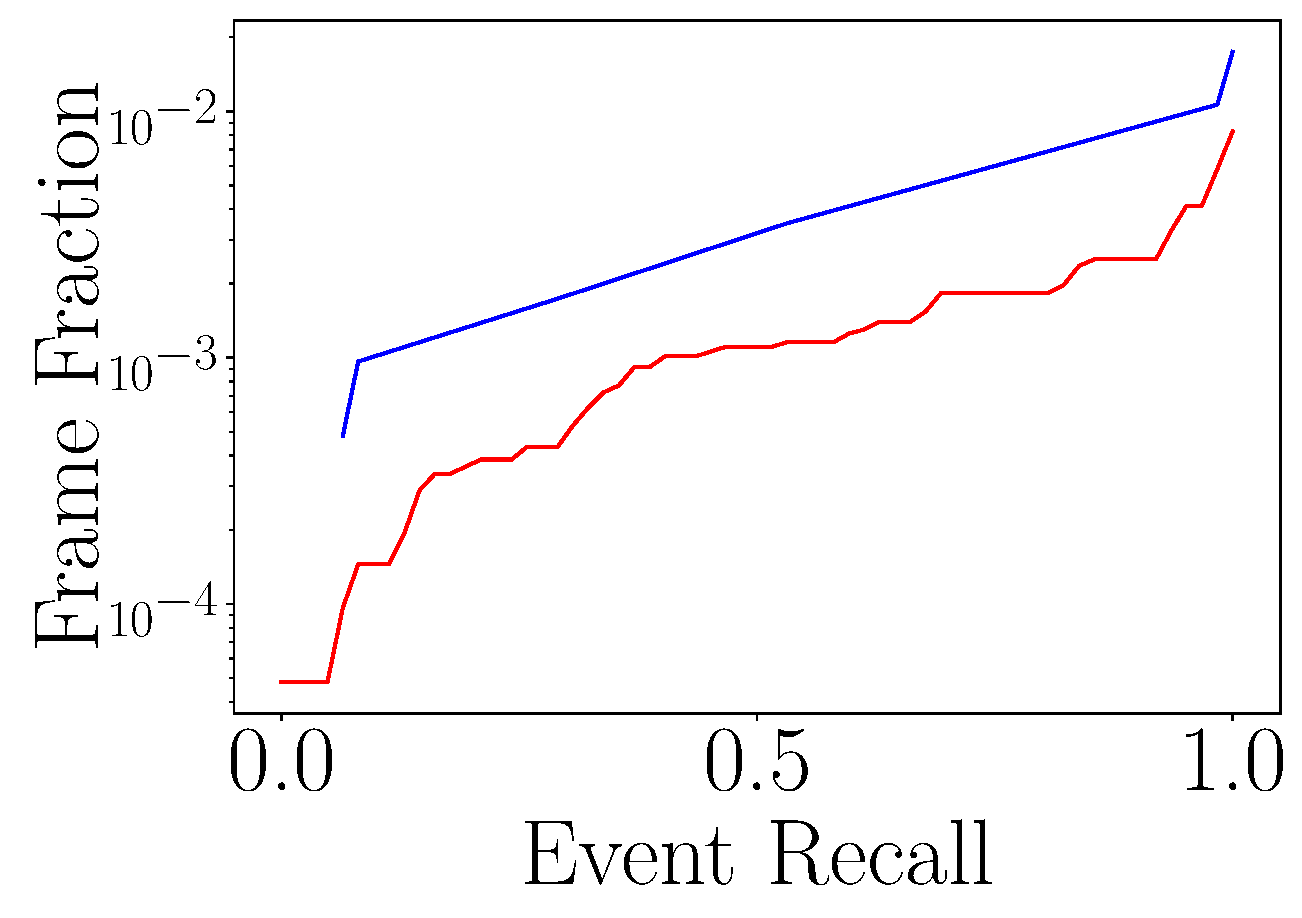
\includegraphics[trim={0.5cm 0.5cm 0 0},clip,width=0.47\linewidth]{FIGS/fig-random-select-and-filter-recall-frame-okutama-aggregated.pdf}}
    \end{subfigure}
    \begin{subfigure}[T2]{
      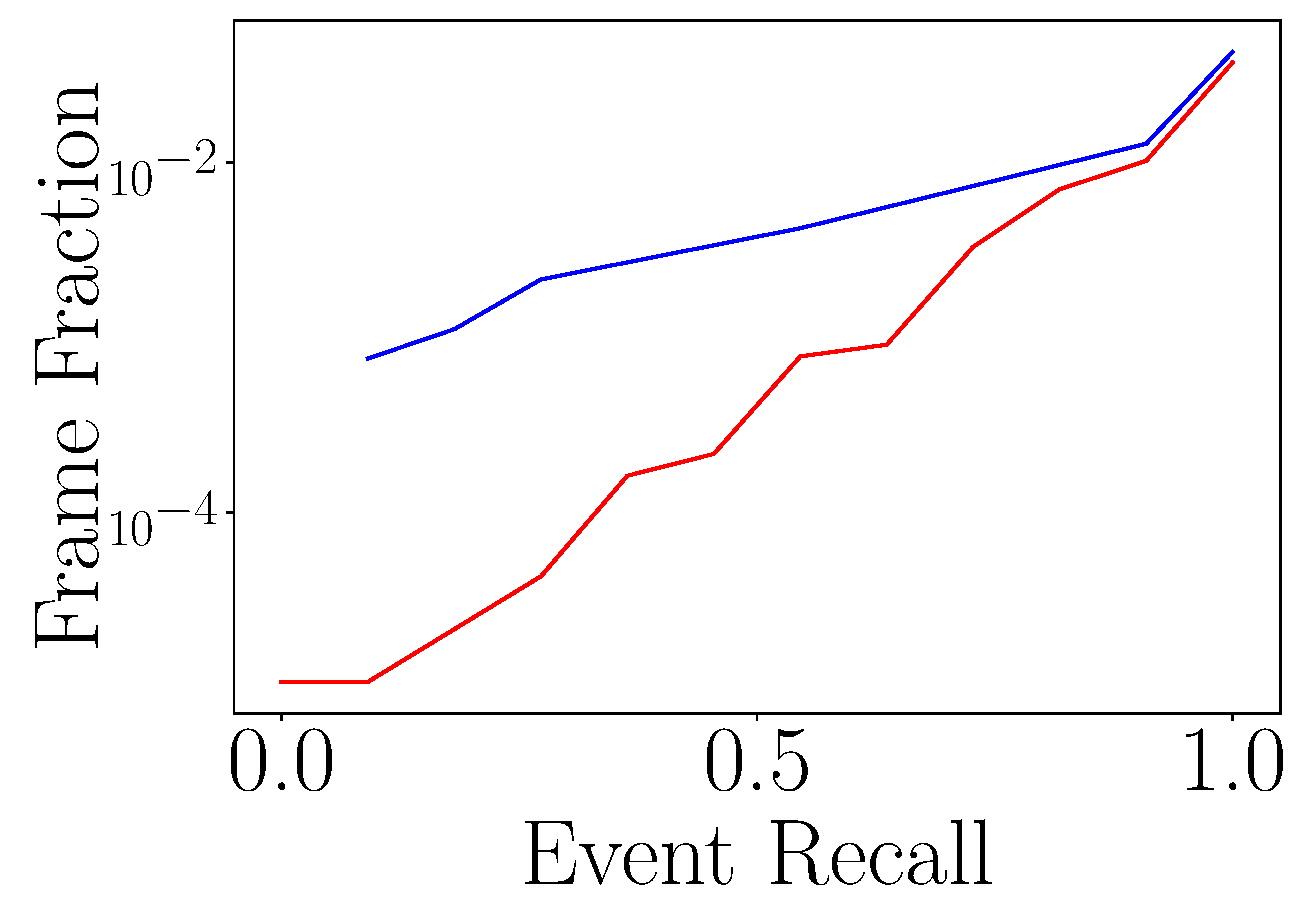
\includegraphics[trim={0.5cm 0.5cm 0 0},clip,width=0.47\linewidth]{FIGS/fig-random-select-and-filter-recall-frame-stanford-aggregated.pdf}}
    \end{subfigure}
    \begin{subfigure}[T3]{
      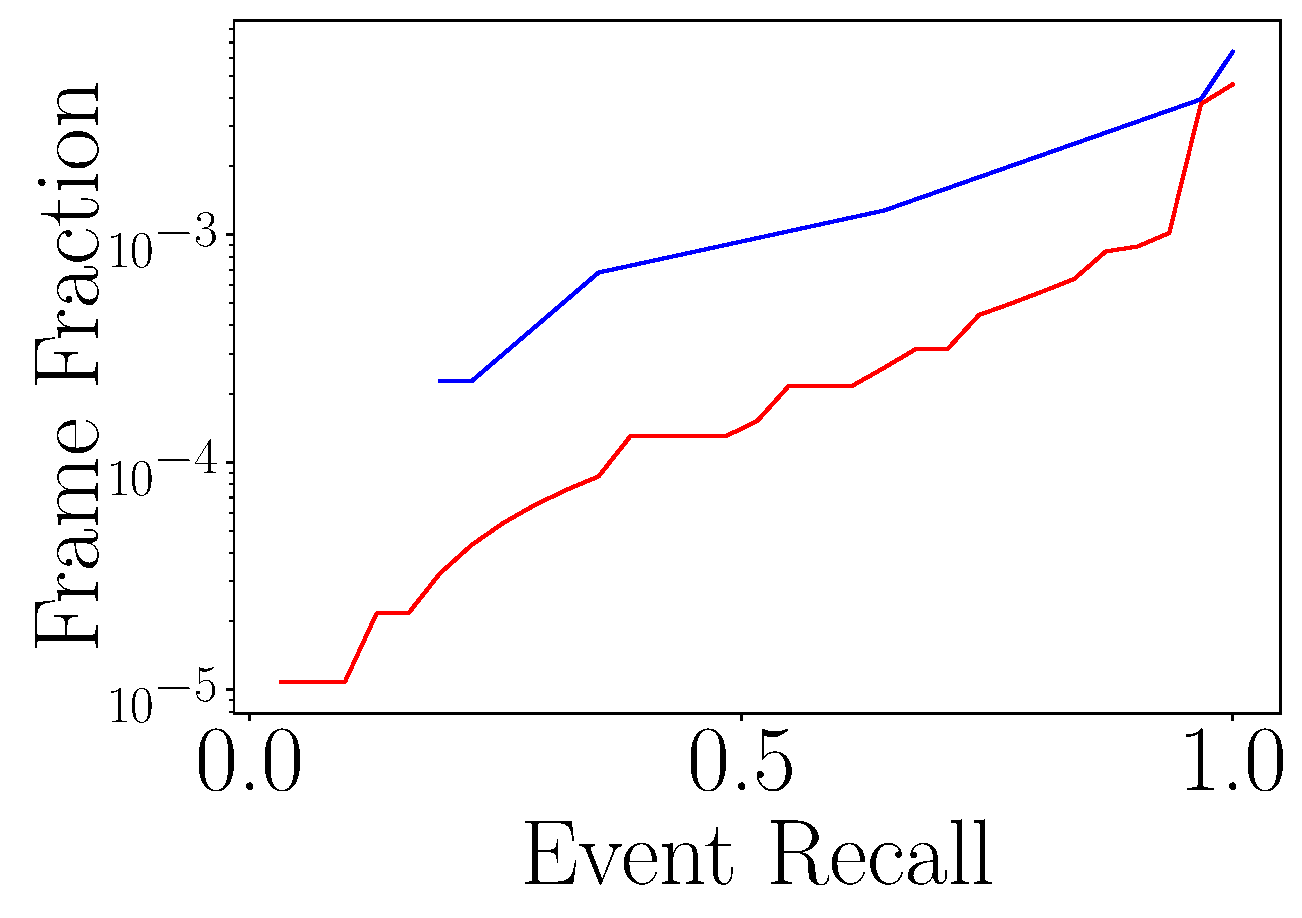
\includegraphics[trim={0.5cm 0.5cm 0 0},clip,width=0.47\linewidth]{FIGS/fig-random-select-and-filter-recall-frame-raft-aggregated.pdf}}
    \end{subfigure}
    \begin{subfigure}[T4]{
      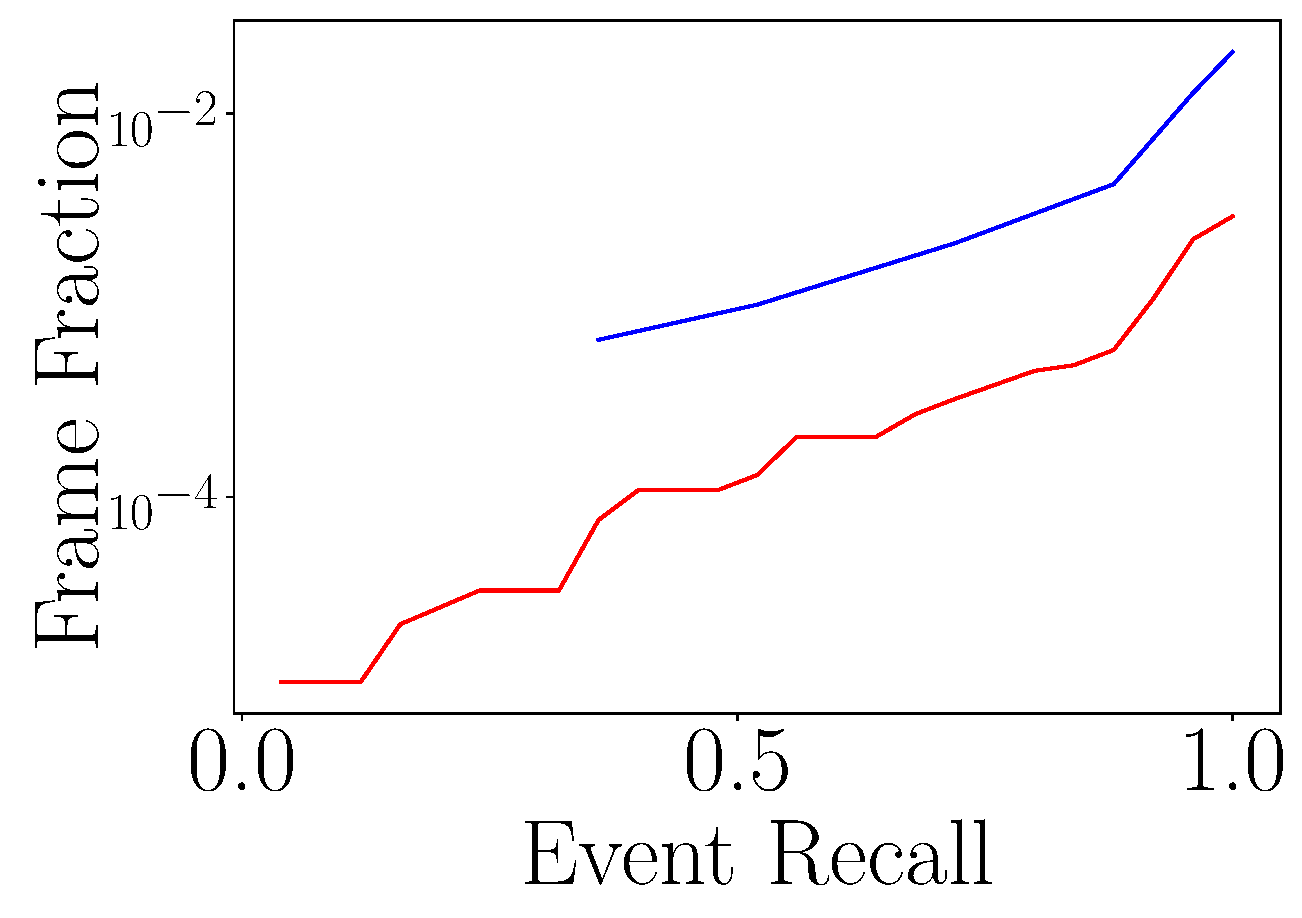
\includegraphics[trim={0.5cm 0.5cm 0 0},clip,width=0.47\linewidth]{FIGS/fig-random-select-and-filter-recall-frame-elephant-aggregated.pdf}}
    \end{subfigure}
    \vspace{-0.15in}
\caption{Sample with Early Discard. Note the log scale on y-axis.}
    \vspace{-0.15in}
\label{fig:sampling-discard}
\end{figure}

Given the relatively low precision of the weak detectors, a significant number 
of false positives are transmitted.  Furthermore, the occurrence of an object will
likely last through many frames, so true positives are also often redundant for 
simple detection tasks.  Both of these result in excessive
consumption of precious bandwidth.  
This suggests that simply restricting the number of transmitted
frames by sampling may help reduce bandwidth consumption.  

Figure~\ref{fig:sampling-only} shows the effects of 
sending a sample of frames from the drone, without any
content-based filtering.  Based on these results, we can reduce
the frames sent as little as one per second and still get
adequate recall at the cloudlet.  Note that this result is very
sensitive to the actual duration of the events in the videos.
For the detection tasks outlined here, most of the events (e.g.,
presences of a particular elephant) last for many seconds (100's
of frames), so such sparse sampling does not hurt recall.
However, if the events were of short duration, e.g., just a few
frames long, then this method would be less effective, as
sampling may lead to many missed events (false negatives).  

Can we use content-based filtering along with sampling to further
reduce bandwidth consumption?  Figure~\ref{fig:sampling-discard}
shows results when running early discard on a sample of the
frames. This shows that for the same recall, we can reduce the
bandwidth consumed by another factor of 5 on average over sampling alone.
This effective combination can reduce the average bandwidth
consumed for our test videos to just a few hundred kilobits
per second.  Furthermore, more processing time is available per
processed frame, allowing more sophisticated algorithms to be
employed, or to allow smaller tiles to be used, improving
accuracy of early discard.  

One case where sampling is not an effective solution is when all
frames containing an object need to be sent to the cloudlet for
some form of activity or behavior analysis from a complete video
sequence (as may be needed for task T5).  In this case, bandwidth
will not reduce much, as all frames in the event sequence must be
sent.  However, the processing time benefits of sampling may
still be exploited, provided all frames in a sample interval are
transmitted on a match.  


\subsection{Effects of Video Encoding}

\begin{figure}
\centering
\begin{tabular}{|p{1.5cm}|p{1.3cm}|p{1.3cm}|p{1.3cm}|}
\hline
JPEG Frame Sequence (MB)  & H264 High Quality (MB)       & H264 Medium Quality (MB) & H264 Low Quality (MB)\\
\hline
5823 & 3549  & 1833 & 147\\
\hline
\end{tabular}\\
\vspace{0.1in}
\begin{captiontext}
H264 high quality uses Constant Rate Factor (CRF) 23. Medium
uses CRF 28 and low uses 40~\cite{Merritt2007}.
\end{captiontext}
\caption{Test Dataset Size With Different Encoding Settings}
\label{fig:video-vs-images}
\end{figure}


One advantage of the {\xc DumbDrone} strategy is that since all
frames are transmitted, one can use a modern video encoding to
reduce transmission bandwidth.  With early discard, only a subset
of disparate frames are sent.  These will likely need to be
individually compressed images, rather than a video stream.  How
much does the switch from video to individual frames affect
bandwidth?  

In theory, this can be a significant impact. Video encoders leverage the
similarity between consecutive frames, and model motion to efficiently encode
the information across a set of frames. Image compression can only exploit
similarity within a frame, and cannot efficiently reduce number of bits needed
to encode redundant content across frames. To evaluate this difference, we start
with extracted JPEG frame sequences of our video data set. We encode the frame
sequence with different H.264 settings. Figure~\ref{fig:video-vs-images}
compares the size of frame sequences in JPEG and the encoded video file sizes.
We see only about 3x difference in the data size for the medium quality. We can
increase the compression (at the expense of quality) very easily, and are able
to reduce the video data rate by another order of magnitude before quality
degrades catastrophically.

However, this compression does affect analytics. Even at medium quality level,
visible compression artifacts, blurring, and motion distortions begin to appear.
Initial experiments analyzing compressed videos show that these distortions do
have a negative impact on accuracy of analytics. Using average precision
analysis, a standard method to evaluate accuracy, we see that the 
most accurate model (Faster-RCNN ResNet101) on low quality videos performs similarly
to the less accurate model (Faster-RCNN InceptionV2) on high quality
JPEG images. This negates the benefits of using the state-of-art models.

In this system, we pay a penalty of sending frames instead of a compressed low
quality video stream. This overhead (approximately 30x) is compensated by the
100x reduction in frames transmitted due to sampling with early discard. In
addition, the selective frame transmission preserves the accuracy of the
state-of-art detection techniques.

Finally, one other option is to treat the set of disparate frames as a sequence
and employ video encoding at high quality. This can ultimately eliminate the per
frame overhead while maintaining accuracy. However, this will require a complex setup with
both low-latency encoders and decoders, which can generate output data
corresponding to a frame as soon as input data is ingested, with no buffering,
and can wait arbitrarily long for additional frame data to arrive. 

For the experiments in the rest of the paper, we only account for the fraction
of frames transmitted, rather than the choice of specific encoding methods used
for those frames.



%-------------- LEAVE THIS AT THE END OF THIS FILE --------------------
\begin{comment}
% Satya: Save this old table because it has lots of details that 
% are not included in the smaller table that is in the paper
\begin{figure*}[]
\centering
\begin{tabular}{|p{2cm}|p{2cm}|p{2cm}|p{3cm}|p{3cm}|p{3cm}|}
\hline
Task                     & Task Description                                                                           & Dataset                & Dataset Description                                                                                                                & Train Videos                                                                                     & Test Videos                                                         \\ \hline
Human Detection 	& Detect human beings in daily life scene. Report any humans detected.			& 	UCF Aerial Action Dataset \href{http://crcv.ucf.edu/data/UCF_Aerial_Action.php}{link}				& A video dataset for aerial view of human actions. 4 videos, 107184 frames in total. 720x480 @ 30FPS. 			&  Select 2 videos with drone moving.  57430 frames.			& Select 2 videos with drone moving. 49754 frames.\\ \hline
Human Detection          & Detect human beings in a search and rescue scene. Report any humans detected.              & Okutama Action Dataset~\cite{Barekatain2017} 	& A video dataset for aerial view concurrent human action detection.  33 videos, 59842 frames in total. 3840x2160 @ 30FPS.           & Select 9 videos in which drones are actively moving, similar to search and rescue. 17763 frames. & Randomly select 3 videos in which drones are moving.  6014 frames.  \\ \hline
Human Activity Detection & Detect human activities such as waving hands                                               & Okutama Action Dataset & Same as above                                                                                                                      & Same as above                                                                                    & Same as above                                                       \\ \hline
Moving Car Detection     & Detect cars in a search and rescue scene that are moving. Report any moving cars detected. & Stanford Drone Dataset~\cite{Robicquet2016} & An aerial video dataset of cars and people navigating in a university campus. 60 videos, 522497 frames in total. $\sim$HD @ 30FPS. & Select 16 videos in which exists moving cars. 179992 frames.                                     & Randomly select 5 videos in which exists moving cars. 60249 frames. \\ \hline
Raft Detection           & Detect raft in a flooding scene                               & Collected 11 Youtube Videos \href{https://www.dropbox.com/sh/zksp1pzc1ix5hlw/AAB3HEhx-yLAJVR1Q3HnFpsWa?dl=0}{[Links]}       & Aerial-view videos with rafts. 11 videos. 54395 frames in total. $\sim$720P @ 30 FPS.                                                                                                    & 8 videos of rafting as training set. 43017 frames.                                      &  3 videos that resemble search and rescue scenarios. 11378 frames.                                               \\ \hline
Animal Detection         & Detect elephants in their natural habitat                     & Collected 11 Youtube Videos \href{https://www.dropbox.com/sh/3uly2qqwbzjasaa/AABiWSzPD_5uzmvCy3meqPKma?dl=0}{[Links]}      &  Aerial-view videos containing elephants in their natural habitat. 11 videos. 54203 frames in total. $\sim$720P @ 30FPS.                                                                         & Randomly selected 8 videos as training set. 39466 frames.                      & Randomly selected 3 videos as test set. 14737 frames.                \\ \hline
\end{tabular}
\caption{Task and Dataset}
\label{fig:task-and-dataset}
\end{figure*}
\end{comment}


\section{{\xc Just-in-time-Learning} S\lc{trategy} To Improve Early Discard}
\label{sec:jitl}

\subsection{Description}

Just-in-time-learning  (JITL) tunes the drone pipeline to the characteristics of
 the current mission in order to reduce transmitted false positives from the
 drone, and therefore reduce wasted bandwidth.  It is inspired by the cascade
 architecture from the computer vision community~\cite{Viola2001}, but is
 different in construction. A JITL filter is a cheap cascade filter that
 distinguishes between the EarlyDiscard DNN's \emph{true positives} (frames that
 are actually interesting) and \emph{false positives} (frames that are wrongly
 considered interesting).  Specifically, when a frame is reported as positive by
 EarlyDiscard, it is then passed through a JITL filter. If the JITL filter
 reports negative, the frame is regarded as a false positive and will not be
 sent. Ideally, all \emph{true positives} from EarlyDiscard are marked
 \emph{positive} by the JITL filter, and all \emph{false positives} from 
 EarlyDiscard are marked \emph{negative}.  Frames dropped by EarlyDiscard are
 not processed by the JITL filter, so this approach can only serve to improve
 precision, but not recall.


Periodically during a drone mission, a JITL filter is trained on the cloudlet
using the frames transmitted from the drone.  The frames received on the
cloudlet are predicted positive by the EarlyDiscard filter. The cloudlet, with
more processing power, is able to run more accurate DNNs to identify true
positives and false positives. Using this information, a small and lightweight
JITL filter is trained to distinguish true positives and false positives of
EarlyDiscard filters. These JITL filters are then pushed to the drone to run as
a cascade filter after the EarlyDiscard DNN.

True/false positive frames have high temporal locality throughout a drone
mission. The JITL filter is expected to pick up the features that confused the
EarlyDiscard DNN in the immediate past and improve the pipeline's accuracy in
the near future. These features are usually specific to the current flight, and
may be affected by terrain, shades, object colors, and particular shapes or
background textures.

JITL can be used with EarlyDiscard DNNs of different cutoff probabilities to
strike different trade-offs. In a bandwidth-favored setting, JITL can work with
an aggressively selective EarlyDiscard DNN to further reduce wasted bandwidth. In
a recall-favored setting, JITL can be used with a lower-cutoff DNN to preserve
recall.

In our implementation, we use a linear support vector machine
(SVM)~\cite{Friedman2001} as the JITL filter. Linear SVM has several advantages:
1) short training time in the order of seconds; 2) fast inference; 3) only
requires a few training examples; 3) small in size to transmit, usually on the
order of 50KB in our experiments. The input features to the JITL SVM filter are
the image features extracted by the EarlyDiscard DNN filter. In our case, since
we are using MobileNet as our EarlyDiscard filter, they are the 1024-dimensional
vector elements from the second last layer of MobileNet. This vector, also
called ``bottleneck values'' or ``transfer values'' captures high-level features
that represents the content of an image. Note that the availability of such
image feature vector is not tied to a particular image classification DNN nor
unique to MobileNet. Most image classification DNNs can be used as a feature
extractor in this way.

\subsection{Experimental Setup}
We used Jetson TX2 as our drone platform and evaluated the JITL strategy on four
tasks, T1 to T4. For the test videos in each task, we began with the
EarlyDiscard filter only and gradually trained and deployed JITL filters.
Specifically, every ten seconds, we trained an SVM using the frames transmitted
from the drone and the ground-truth labels for these frames. In a real
deployment, the frames would be marked as true positives or false positives by
an accurate DNN running on the cloudlet since ground-truth labels are not
available. In our experiments, we used ground-truth labels to control variables
and remove the effect of imperfect prediction of DNN models running on the
cloudlet. In addition, we used the true and false positives from all previous
intervals, not just the last ten seconds when training the SVM. The SVM, once
trained, is used as a cascade filter running after the EarlyDiscard filter on
the drone to predict whether the output of the EarlyDiscard filter is correct or
not. For a frame, if the EarlyDiscard filter predicts it to be interesting, but
the JITL filter predicts the EarlyDiscard filter is wrong, it would not be
transmitted to the cloudlet. In other words, following two criteria need to be
satisfied for a frame to be transmitted to the cloudlet: 1) EarlyDiscard filter
predicts it to be interesting 2) JITL filter predicts the EarlyDiscard filter is
correct on this frame.

\subsection{Results}

%\noindent{\textbf{Frame transmission and DNN cutoff}}
%In this experiment, we vary the cutoff probability of the DNN that runs before the JITL filter.
%For each dataset,
%we report the number of total transmitted frames and the number of transmitted true positive frames.
%For comparison, we also report the DNN's number when JITL is not activated.
%Figure \ref{fig:jitl-frame-cutoff} shows the results.
%In most cases, JITL helps reducing the total transmitted frames without significantly reducing true positives.
%T5 manifests the best example: JITL retains almost all true positives,
%while reducing total transmission observably.

%\begin{figure}
%\centering
%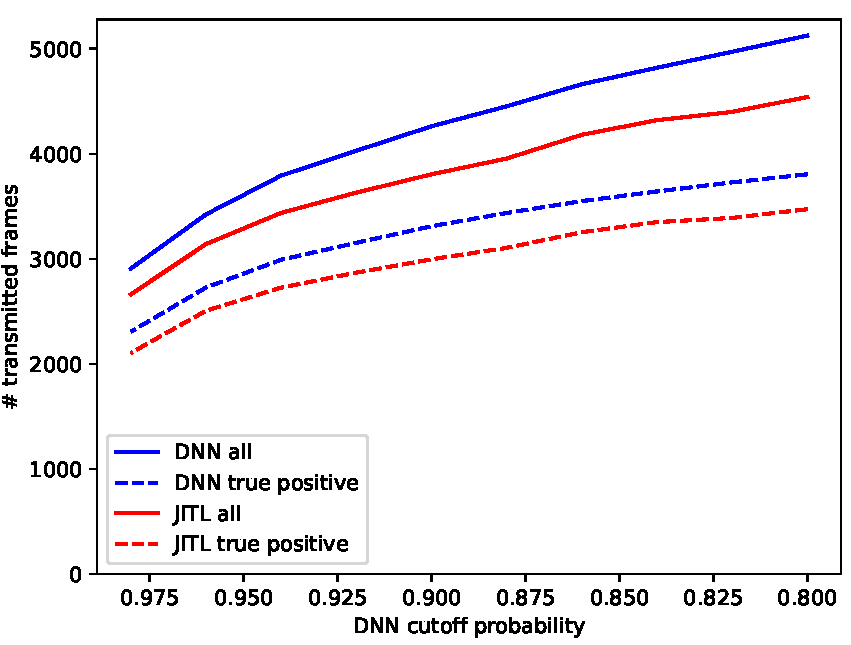
\includegraphics[width=0.6\linewidth]{FIGS/fig-jitl-okutama-frame.pdf}\\
%(a) T1\\[0.1in]
%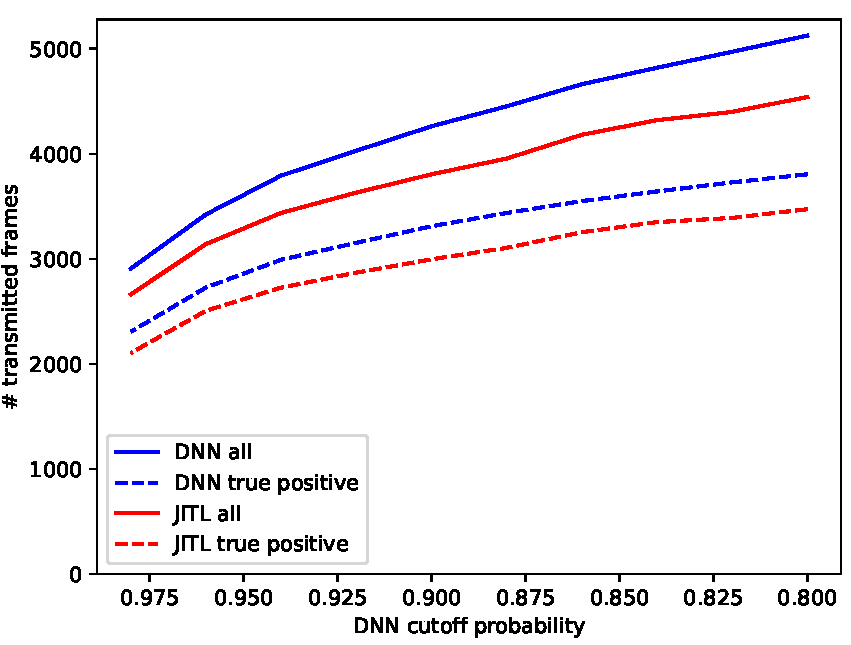
\includegraphics[width=0.6\linewidth]{FIGS/fig-jitl-okutama-frame.pdf}\\
%(b) T3\\[0.1in]
%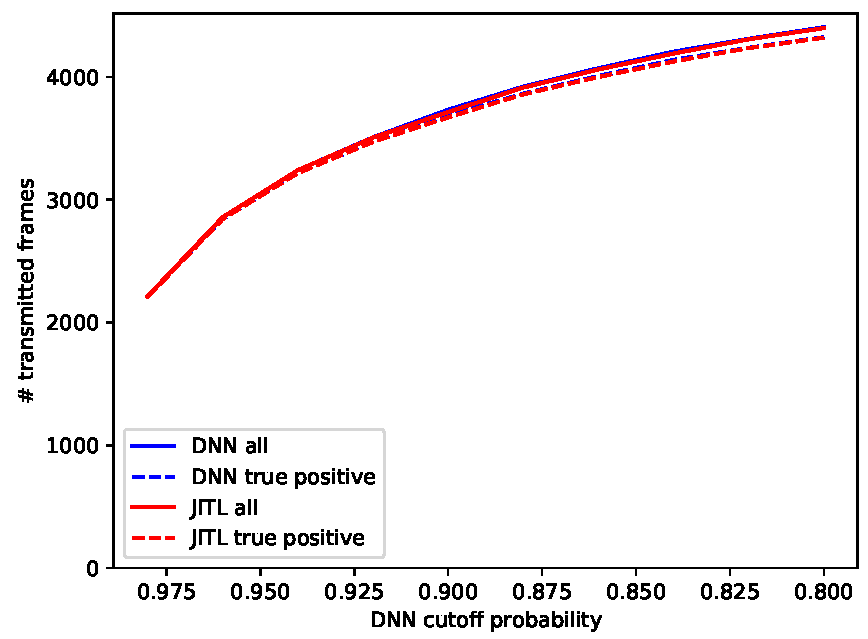
\includegraphics[width=0.6\linewidth]{FIGS/fig-jitl-raft-frame.pdf}\\
%(c) T4\\[0.1in]
%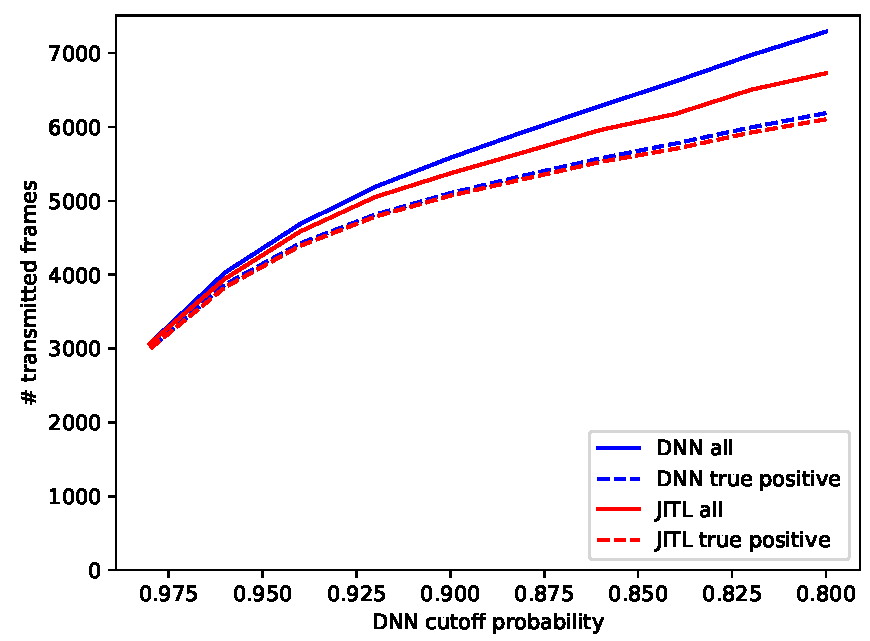
\includegraphics[width=0.6\linewidth]{FIGS/fig-jitl-elephant-frame.pdf}\\
%(d) T5\\[0.1in]
%\caption{Bandwidth vs. DNN Cutoff}
%\label{fig:jitl-frame-cutoff}
%\end{figure}


From our experiments, JITL is able to filter out more than 15\% of remaining
frames after EarlyDiscard without loss of event recall for three of four tasks.
Figure~\ref{fig:jitl-eventrecall} details the fraction of frames saved by JITL.
The x-axis presents event recall. Y-axis represents the fraction of total
frames. The blue region presents the achievable fraction of frames by
EarlyDiscard. The orange region shows the additional savings using JITL. For T1,
T3, and T4, at the highest event recall, JITL filters out more than 15\% of
remaining frames. This shows that JITL is effective at reducing the false
positives thus improving the precision of the drone filter. However,
occasionally, JITL predicts wrongly and removes true positives. For example, for
T2, JITL does not achieve a perfect event recall. This is due to shorter event
duration in T2, which results in fewer positive training examples to learn
from. Depending on tasks, getting enough positive training examples for JITL
could be difficult, especially when events are short or occurrences are few. To
overcome this problem in practice, techniques such as synthetic data
generation~\cite{Dwibedi2017} could be explored to synthesize true positives
from the background of the current flight.

\begin{figure}
    \centering
    
\includegraphics[trim={0 1.8cm 0 0},clip,width=0.7\linewidth]{FIGS/fig-jitl-legend.pdf}
    \hspace*{-0.3in}
    \begin{subfigure}[T1]{
        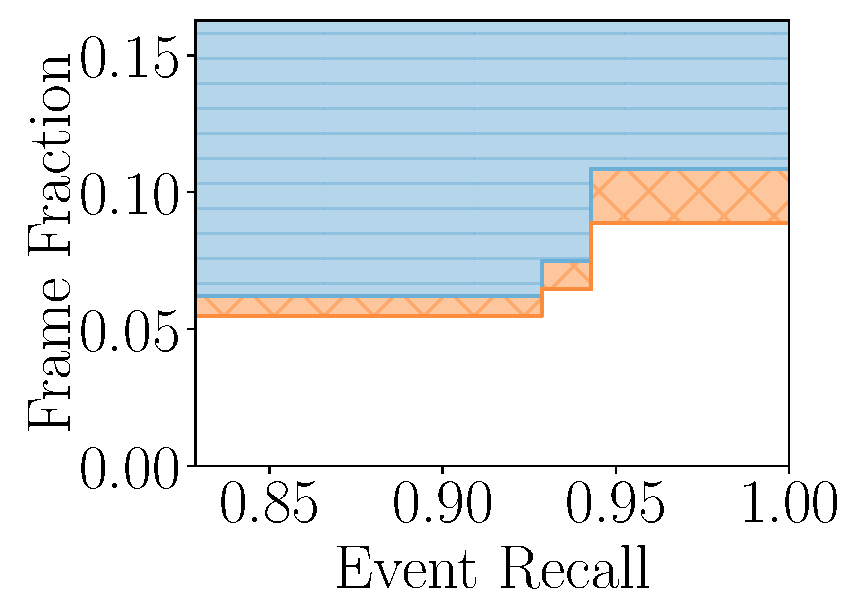
\includegraphics[width=0.5\linewidth]{FIGS/fig-jitl-okutama-eventrecall-step.pdf}}
    \end{subfigure}
    \begin{subfigure}[T2]{
        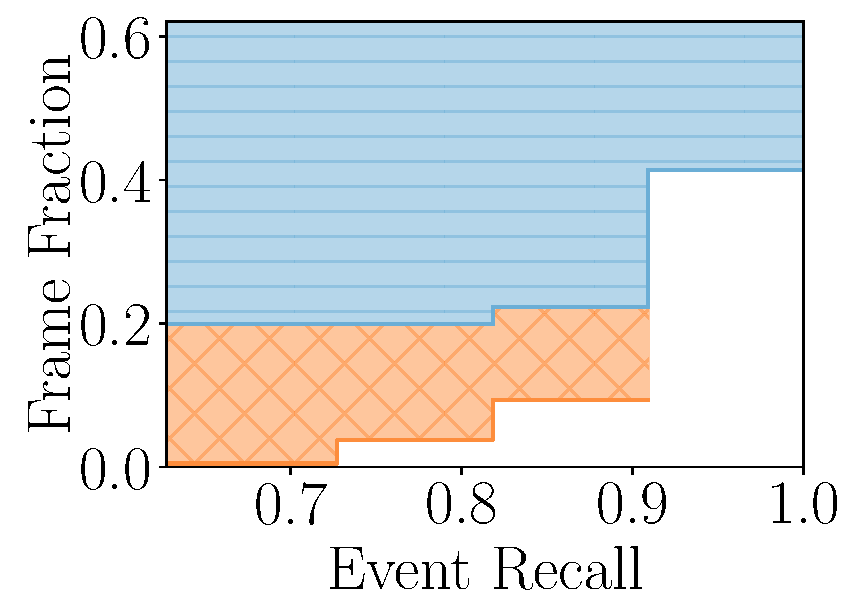
\includegraphics[width=0.5\linewidth]{FIGS/fig-jitl-stanford-eventrecall-step.pdf}}
    \end{subfigure}
    \hspace*{-0.3in}
    \begin{subfigure}[T3]{
        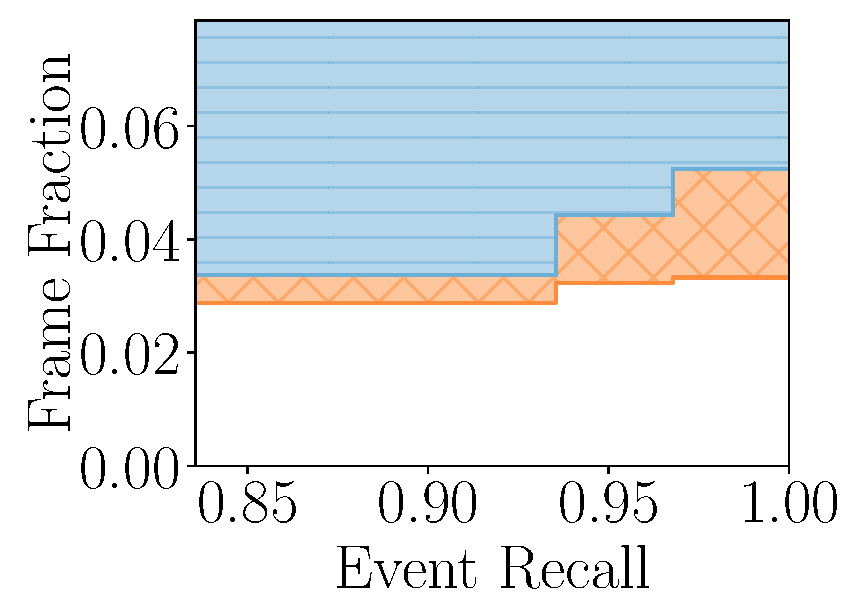
\includegraphics[width=0.5\linewidth]{FIGS/fig-jitl-raft-eventrecall-step.pdf}}
    \end{subfigure}
    \begin{subfigure}[T4]{
        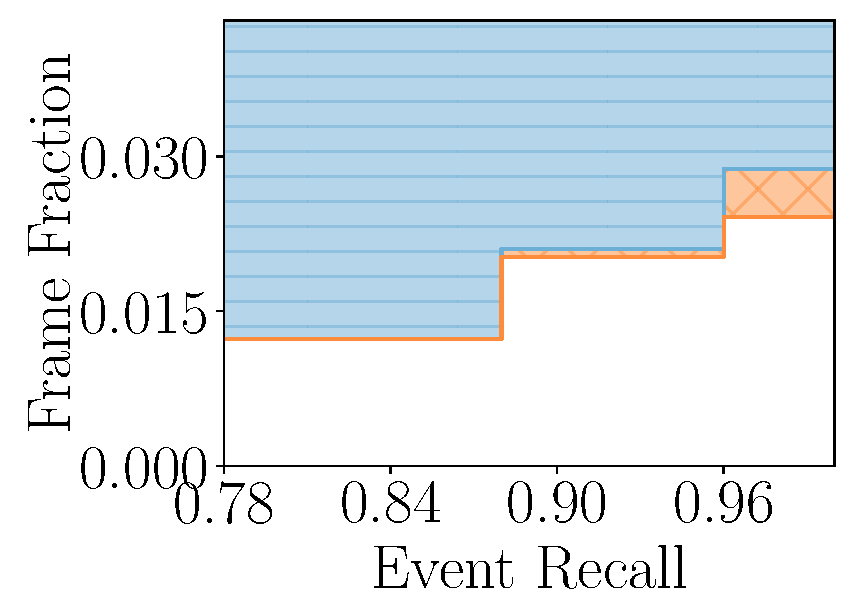
\includegraphics[width=0.5\linewidth]{FIGS/fig-jitl-elephant-eventrecall-step.pdf}}
    \end{subfigure}
\caption{JITL Fraction of Frames under Different Event Recall}
\label{fig:jitl-eventrecall}
\end{figure}

\section{Evaluation}
\section{Discussion}
\chapter{Application-Aware Techniques to Reduce Offered Load}
\label{chapter: load}

{\em Elasticity} is a key attribute of cloud computing.  When load
rises, new servers can be rapidly spun up.  When load subsides, idle
servers can be quiesced to save energy.  Elasticity is vital to
scalability, because it ensures acceptable response times under a wide
range of operating conditions.  To benefit, cloud services need to be
architected to easily scale out to more servers.  Such a design is
said to be ``cloud-native.''

In contrast, edge computing has limited elasticity.  As its name implies, a
cloudlet is designed for much smaller physical space and electrical power than a
cloud data center.  Hence, the sudden arrival of an unexpected flash crowd can
overwhelm a cloudlet.  Since low end-to-end latency is a prime reason for edge
computing, shifting load elsewhere (e.g., the cloud) is not an attractive
solution.  {\em How do we build multi-user edge computing systems that preserve
low latency even as load increases?}  That is the focus of the next two chapters.

Our approach to scalability is driven by the following observation. Since
compute resources at the edge cannot be increased on demand, the only paths to
scalability are (a) to reduce offered load, as discussed in this chapter,
or (b) to reduce queueing delays through improved end-to-end scheduling,
as discussed in Chapter~\ref{chapter: cloudlet}.  Otherwise, the mismatch between
resource availability and offered load will lead to increased queueing delays
and hence increased end-to-end latency.  Both paths require the average burden
placed by each user on the cloudlet to fall as the number of users increases.
This, in turn, implies {\em adaptive application behavior} based on guidance
received from the cloudlet or inferred by the user's mobile device.  In the
context of Figure~\ref{fig:3tier}, scalability at the left is achieved very
differently from scalability at the right.  The relationship between Tier-3 and
Tier-2 is {\em non-workload-conserving}, while that between Tier-1 and other
tiers is workload-conserving.

While we demonstrated application-agnostic techniques to reduce network
transmission between Tier-3 and Tier-2 in Chapter~\ref{chapter: bandwidth},
offered load can be further reduced with application assistance. We claim that
scalability at the edge can be better achieved for applications that have been
designed with this goal in mind.  We refer to applications that are specifically
written to leverage edge infrastructure as {\em edge-native applications.} These
applications are deeply dependent on the services that are only available at the
edge (such as low-latency offloading of compute, or real-time access to video
streams from edge-located cameras), and are written to adapt to
scalability-relevant guidance.  For example, an application at Tier-3 may be
written to offload object recognition in a video frame to Tier-2, but it may
also be prepared for the return code to indicate that a less accurate (and hence
less compute-intensive) algorithm than normal was used because Tier-2 is heavily
loaded.  Alternatively, Tier-2 or Tier-3 may determine that the wireless channel
is congested; based on this guidance, Tier-3 may reduce offered load by
preprocessing a video frame and using the result to decide whether it is
worthwhile to offload further processing of that frame to the cloudlet.  Several
earlier work~\cite{Hu2015}~\cite{christensen2019towards} have shown that even
modest computation, such as color filtering and shallow DNN processing, at Tier-3
can make surprisingly good predictions about whether a specific use of Tier-2 is
likely to be worthwhile.

Edge-native applications may also use {\em cross-layer adaptation
  strategies,} by which knowledge from Tier-3 or Tier-2 is used in the
management of the wireless channel between them.  For example, an
assistive augmented reality (AR) application that verbally guides a
visually-impaired person may be competing for the wireless channel and
cloudlet resources with a group of AR gamers.  In an overload
situation, one may wish to favor the assistive application over the
gamers.  This knowledge can be used by the cloudlet operating system
to preferentially schedule the more important workload.  It can also
be used for prioritizing network traffic by using {\em fine-grain
  network slicing,} as envisioned in 5G~\cite{Contreras2018}.

Wearable cognitive assistance, perceived to be ``killer apps'' for edge
computing, are perfect exemplars of edge-native applications. In the rest of
this chapter, we showcase how we can leverage unique application characteristics
of WCAs to adapt application behavior and reduce offered load. Our work is built
on the Gabriel platform~\cite{ha2014towards,chen2017empirical}, shown in
Figure~\ref{fig:gabriel}. The Gabriel front-end on a wearable device performs
preprocessing of sensor data (e.g., compression and encoding), which it streams
over a wireless network to a cloudlet. We refer to the Gabriel platform with new
mechanisms that handle multitenancy, perform resource allocation, and support
application-aware adaptation as ``Scalable Gabriel'' and the single-user
baseline platform as ``Original Gabriel''.

% The Gabriel back-end on the cloudlet has
% a modular structure. The {\em control module} is the focal point for all
% interactions with the wearable device.  A publish-subscribe (PubSub) mechanism
% decodes and distributes the incoming sensor streams to multiple {\em cognitive
% modules} (e.g., task-specific computer vision algorithms) for concurrent
% processing. Cognitive module outputs are integrated by a task-specific {\em user
% guidance module} that performs higher-level cognitive processing such as
% inferring task state, detecting errors, and generating guidance in one or more
% modalities (e.g., audio, video, text, etc.).

% It did,
% however, have a token-based transmission mechanism.  This limited a client to
% only a small number of outstanding operations, thereby offering a simple form of
% rate adaptation to processing or network bottlenecks.  We have retained this
% token mechanism in our system. In addition, 


% Since the techniques for reducing offered workload are application-specific, we
% focus on a specific class of edge-native applications to validate our ideas.
% Our choice is a class of applications called {\em Wearable Cognitive Assistance}
% (WCA) applications~\cite{ha2014towards}.  They are perceived to be ``killer apps'' for
% edge computing because (a) they transmit large volumes of video data to the
% cloudlet; (b) they have stringent end-to-end latency requirements; and (c) they
% make substantial compute demands of the cloudlet, often requiring high-end GPUs.

% We leverage unique characteristics of WCA applications to reduce
% offered load through graceful degradation and improved resource
% allocation.  Our contributions are as follows:
% \begin{smitemize}
%   \item{An architectural framework for WCA that enables graceful degradation under heavy load.}
%   \item{An adaptation taxonomy of WCA applications, and techniques for workload reduction.}
%   \item{A cloudlet resource allocation scheme based on degradation heuristics and external policies.}
%   \item{A prototype implementation of the above.}
%   \item{Experimental results showing up to 40\% reduction in offered load and graceful degradation in oversubscribed edge systems.}
% \end{smitemize}

\section{Adaptation Architecture and Strategy}

\begin{figure}[h]
\centering
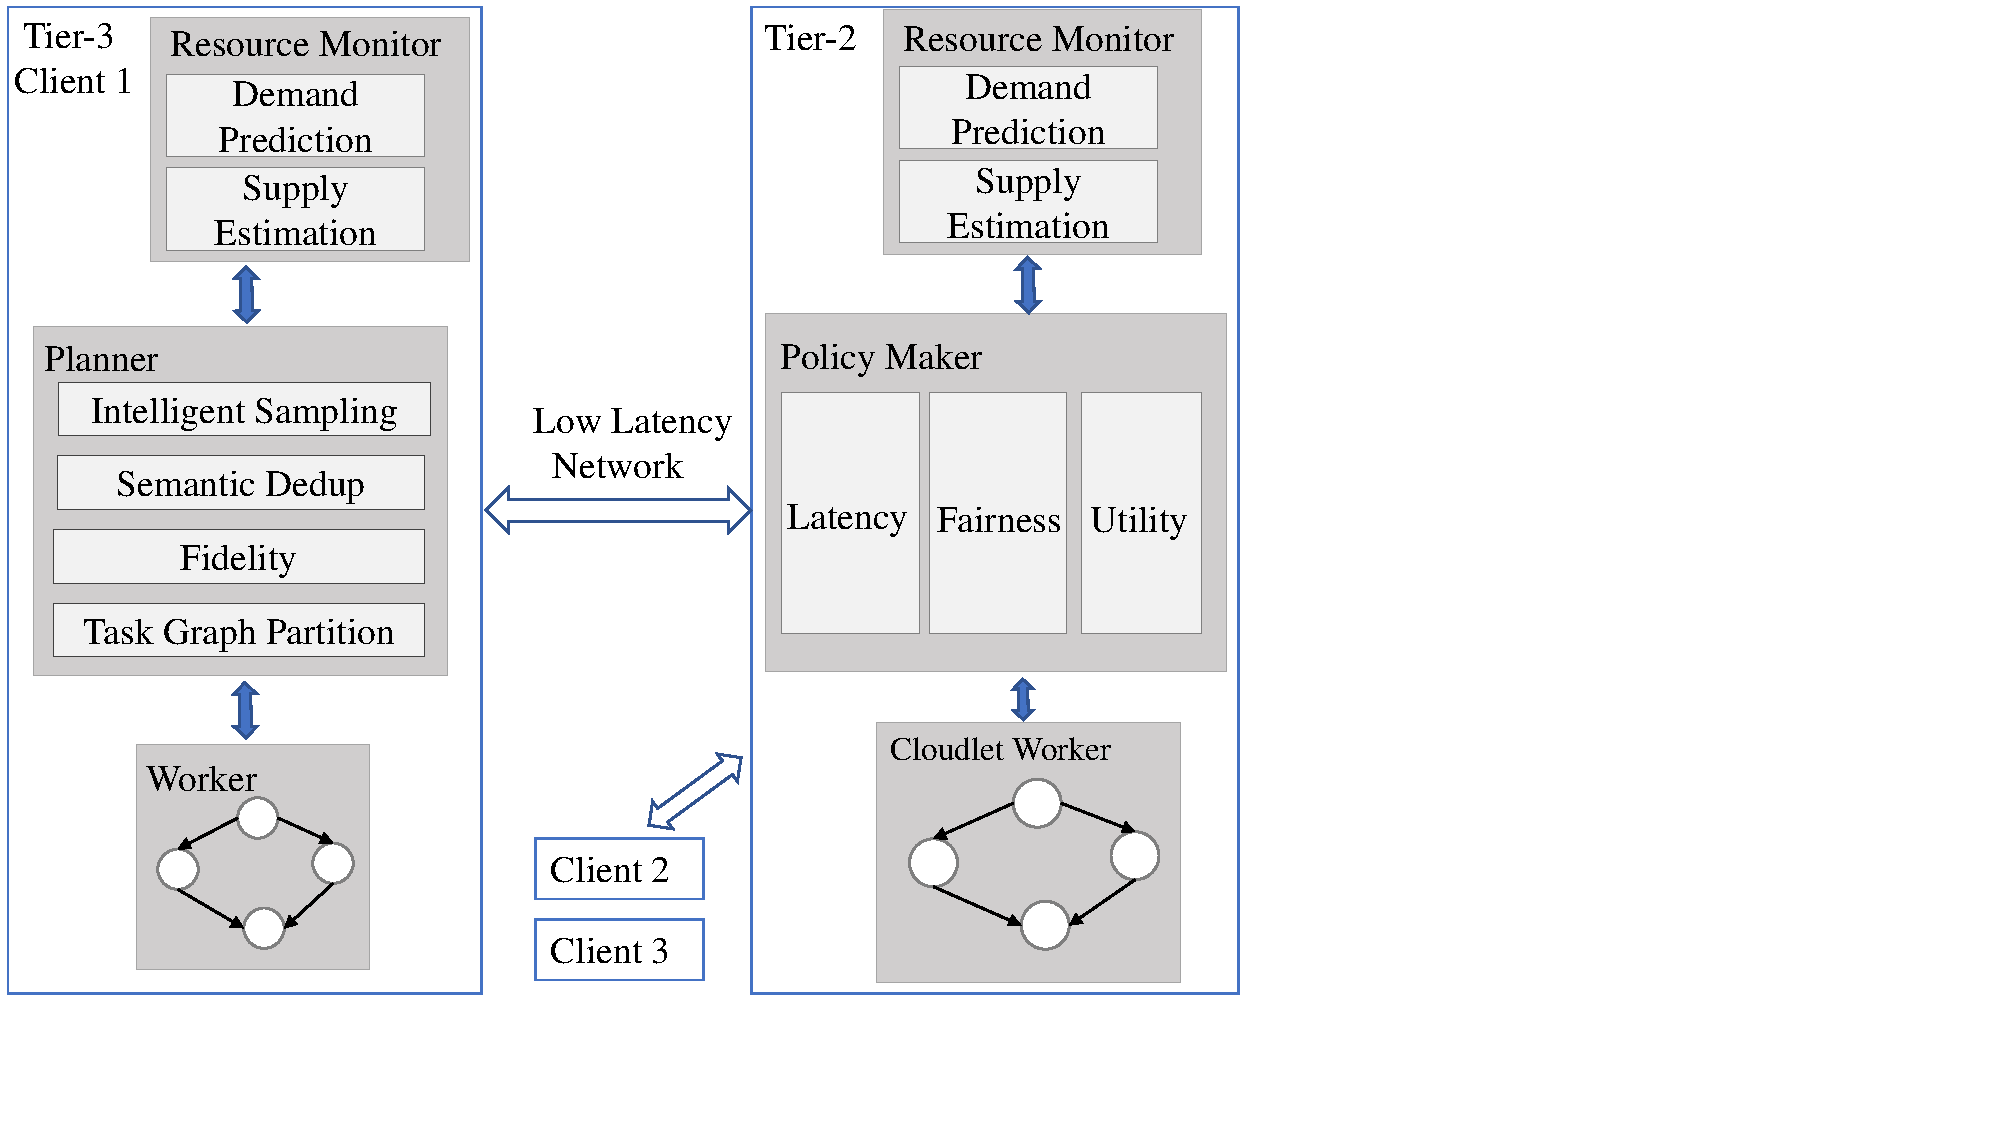
\includegraphics[width=\textwidth,trim=0 3em 11cm 0, clip]{FIGS/arch-vertical.pdf}
\vspace{-0.3in}
\caption{Adaptation Architecture}
\label{fig:arch}
\end{figure}

The original Gabriel platform has been validated in meeting the latency bounds
of WCA applications in single-user settings~\cite{chen2017empirical}.  Scalable
Gabriel aims to meet these latency bounds in multi-user settings, and to ensure
performant multitenancy even in the face of overload.  We take two complementary
approaches to scalability.  The first is for applications to reduce their
offered load to the wireless network and the cloudlet through adaptation.  The
second uses end-to-end scheduling of cloudlet resources to minimize queueing and
impacts of overload (See Chapter~\ref{chapter: cloudlet} for more details).  We
both approaches, and combine them using the system architecture shown in
Figure~\ref{fig:arch}.  We assume benevolent and collaborative clients in the
system.

\section{System Architecture}

Computer vision processing is at the core of wearable cognitive assistance. We
consider scenarios in which multiple Tier-3 devices concurrently offload their
vision processing to a single cloudlet over a shared wireless network.  The
devices and cloudlet work together to adapt workloads to ensure good performance
across all of the applications vying for the limited Tier-2 resources and
wireless bandwidth.  This is reflected in the system architecture shown in
Figure~\ref{fig:arch}.

Monitoring of resources is done at both Tier-3 and Tier-2.  Certain
resources, such as battery level, are device-specific and can only be
monitored at Tier-3.  Other shared resources can only be monitored at
Tier-2: these include processing cores, memory, and GPU.  Wireless
bandwidth and latency are measured independently at Tier-3 and Tier-2,
and aggregated to achieve better estimates of network conditions.

This information is combined with additional high-level predictive knowledge and
factored into scheduling and adaptation decisions.  The predictive knowledge
could arise at the cloudlet (e.g., arrival of a new device, or imminent change
in resource allocations), or at the Tier-3 device (e.g., application-specific,
short-term prediction of resource demand).  All of this information is fed to a
{\em policy module} running on the cloudlet.  This module is guided by an
external policy specification and determines how cloudlet resources should be
allocated across competing Tier-3 applications.  Such policies can factor in
latency needs and fairness, or simple priorities (e.g., a blind person
navigation assistant may get priority over an AR game).

A {\em planner module} on the Tier-3 device uses current resource
utilization and predicted short-term processing demand to determine
which workload reduction techniques (described in
Section~\ref{sec:workload-reduction}) should be applied to achieve
best performance for the particular application given the resource
allocations.

\begin{table*}[]
    \begin{tabular}{|r|p{25ex}|p{30ex}|p{25ex}|}
    \hline&&&\\[0.1in]
    &{\normalsize\bf Question}  & {\normalsize\bf Example} & {\normalsize\bf Load-reduction Technique} \\
    & & & \\ 
    \hline
    1&How often are instructions given, compared to task duration? 
        & Instructions for each step in IKEA lamp assembly are 
            rare compared to the total task time, e.g., 6 instructions over 
            a 10 minute task.
        & Enable adaptive sampling based on active and passive phases. \\ \hline
    2&Is intermittent processing of input frames sufficient for giving instructions?
        & Recognizing a face in any one frame is sufficient for
whispering the person's name.
        & Select and process key frames.  \\ \hline
    3&Will a user wait for system responses before proceeding?  
        & A first-time user of a medical device will pause until  an instruction is received.
        & Select and process key frames. \\ \hline
    4&Does the user have a pre-defined workspace in the scene?
        & Lego pieces are assembled on the lego board. Information outside the board can
             be safely ignored.
        & Focus processing attention on the region of interest. \\ \hline
    5&Does the vision processing involve identifying and locating objects?
        & Identifying a toy lettuce for a toy sandwich.
        & Use tracking as cheap approximation for detection. \\ \hline
    6&Are the vision processing algorithms insensitive to image resolution?
        & Many image classification DNNs limit resolutions to  
            the size of their input layers.
        & Downscale sampled frames on device before transmission.    \\ \hline
    7&Can the vision processing algorithm trade off accuracy and computation? 
        & Image classification DNN MobileNet is computationally cheaper than ResNet, but less accurate. 
        & Change computation fidelity based on resource utilization. \\ \hline
    % 8&Is there inherent human-level latency for a state change?
    %     & It takes at least a few seconds for a human to drill a hole.
    %     & Frame sampling and processing suppression based on heuristics   \\ \hline
    8&Can IMUs be used to identify the start and end of user activities?
        & User's head movement is significantly larger when searching for a Lego block.
        & Enable IMU-based frame suppression. \\ \hline
    9&Is the Tier-3 device powerful enough to run parts of the processing pipeline?
        & A Jetson TX2 can run MobileNet-based image recognition in real-time.
        & Partition the vision pipeline between Tier-3 and Tier-2.   \\ \hline
    \end{tabular}
\vspace{0.1in}
    \caption{Application characteristics and corresponding applicable techniques to reduce load}
    \label{tab:questions-techniques}
\end{table*}

\section{Adaptation Goals}
 
For WCAs, the dominant class of offloaded computations are computer vision
operations, e.g., object detection with deep neural networks (DNNs), or activity
recognition on video segments. The interactive nature of these applications
precludes the use of deep pipelining that is commonly used to improve the
efficiency of streaming analytics.  Here, end-to-end latency of an individual
operation is more important than throughput. Further, it is not just the mean or
median of latency, but also the tail of the distribution that matters.  There is
also significant evidence that user experience is negatively affected by
unpredictable variability in response times. Hence, a small mean with short tail
is the desired ideal. Finally, different applications have varying degrees of
benefit or utility at different levels of latency.  Thus, our adaptation
strategy incorporates application-specific utility as a function of latency as
well as policies maximizing the total utility of the system.


\section{Leveraging Application Characteristics}
\label{sec:workload-reduction}

WCA applications exhibit certain properties that distinguish them from
other video analytics applications studied in the past.  Adaptation
based on these attributes provides a unique opportunity to improve
scalability.

\textbf{Human-Centric Timing:} The frequency and speed with which guidance must
be provided in a WCA application often depends on the speed at which the human
performs a task step.  Generally, additional guidance is not needed until the
instructed action has been completed. For example, in the RibLoc assistant
(Chapter~\ref{chapter: background}), drilling a hole in bone can take several
minutes to complete.  During the drilling, no further guidance is provided after
the initial instruction to drill.  Inherently, these applications contain {\em
active phases,} during which an application needs to sample and process video
frames as fast as possible to provide timely guidance, and {\em passive phases,}
during which the human user is busy performing the instructed step.  During a
passive phase, the application can be limited to sampling video frames at a low
rate to determine when the user has completed or nearly completed the step, and
may need guidance soon.  Although durations of human operations need to be
considered random variables, many have empirical lower bounds.  Adapting
sampling and processing rates to match these active and passive phases can
greatly reduce offered load.  Further, the offered load across users is likely
to be uncorrelated because they are working on different tasks or different
steps of the same task. If inadvertent synchronization occurs, it can be broken
by introducing small randomized delays in the task guidance to different users.
These observations suggest that proper end-to-end scheduling can enable
effective use of cloudlet resources even with multiple concurrent applications.

\textbf{Event-Centric Redundancy}: In many WCA applications, guidance
is given when a user event causes visible state change. For example,
placing a lamp base on a table triggers the IKEA Lamp application to
deliver the next assembly instruction.  Typically, the application
needs to process video at high frame rate to ensure that such state
change is detected promptly, leading to further guidance.  However,
all subsequent frames will continue to reflect this change, and are
essentially redundant, wasting wireless and computing resources.
Early detection of redundant frames through careful semantic
deduplication and frame selection at Tier-3 can reduce the use of
wireless bandwidth and cloudlet cycles on frames that show no
task-relevant change.

\textbf{Inherent Multi-Fidelity}: Many vision processing algorithms
can tradeoff fidelity and computation.  For example, frame resolution
can be lowered, or a less sophisticated DNN used for inference, in
order to reduce processing at the cost of lower accuracy.  In many
applications, a lower frame rate can be used, saving computation and
bandwidth at the expense of response latency.  Thus, when a cloudlet
is burdened with multiple concurrent applications, there is scope to
select operating parameters to keep computational load manageable.
Exactly how to do so may be application-dependent.  In some cases,
user experience benefits from a trade-off that preserves fast response
times even with occasional glitches in functionality.  For others,
e.g., safety-critical applications, it may not be possible to
sacrifice latency or accuracy.  This in turn, translates to lowered
scalability of the latter class of application, and hence the need for
a more powerful cloudlet and possibly different wireless technology to
service multiple users.

\begin{figure}[h]
    \centering
    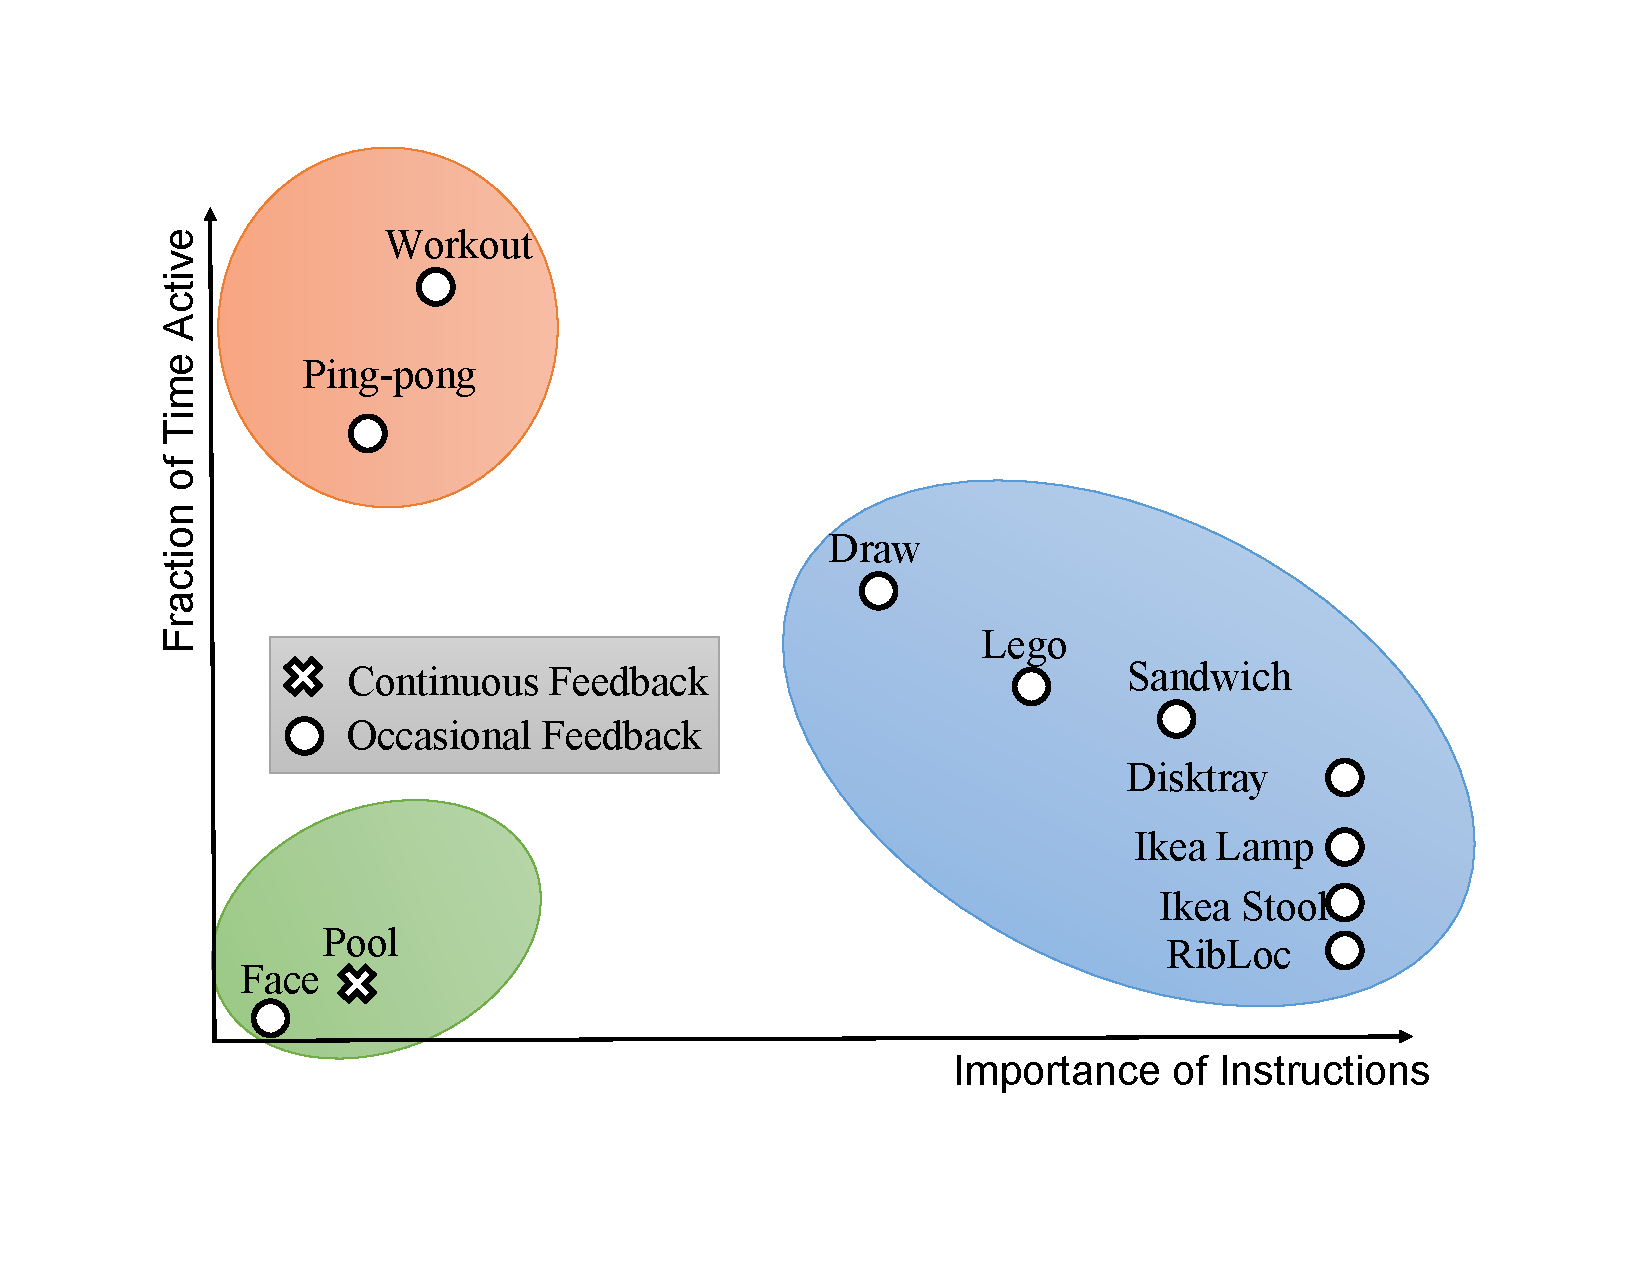
\includegraphics[width=\linewidth, trim=10em 2em 6em 2em, clip]{FIGS/fig-design-space.pdf}
    \caption{Design Space of WCA Applications}
    \label{figs:design-space}
\end{figure}
\subsection{Adaptation-Relevant Taxonomy}

\label{sec:taxonomy}

The characteristics described in the previous section largely hold for
a broad range of WCA applications.  However, the degree to which
particular aspects are appropriate to use for effective adaptation is
very application dependent, and requires a more detailed
characterization of each application.  To this end, our system
requests a manifest describing an application from the developers.
This manifest is a set of yes/no or short numerical responses to the
questions in Table~\ref{tab:questions-techniques}.  Using these, we
construct a taxonomy of WCA applications (shown in
Figure~\ref{figs:design-space}), based on clusters of applications along
dimensions induced from the checklist of questions.  In this case, we
consider two dimensions -- the fraction of time spent in "active"
phase, and the significance of the provided guidance (from merely
advisory, to critical instructions).  Our system varies the adaptation
techniques employed to the different clusters of applications.  We
note that as more applications and more adaptation techniques are
created, the list of questions can be extended, and the taxonomy can be
expanded.

\section{Adaptive Sampling}

The processing demands and latency bounds of a WCA application can
vary considerably during task execution because of human speed
limitations.  When the user is awaiting guidance, it is desirable to
sample input at the highest rate to rapidly determine task state and
thus minimize guidance latency.  However, while the user is performing
a task step, the application can stay in a passive state and sample at
a lower rate.  For a short period of time immediately after guidance
is given, the sampling rate can be very low because it is not humanly
possible to be done with the step.  As more time elapses, the
sampling rate has to increase because the user may be nearing
completion of the step.  Although this active-passive phase
distinction is most characteristic of WCA applications that provide
step-by-step task guidance (the blue cluster in
the lower right of Figure~\ref{figs:design-space}), most WCA
applications exhibit this behavior to some degree.  As shown in the
rest of this section, adaptive sampling rates can reduce processing
load without impacting application latency or accuracy.

We use task-specific heuristics to define application active and
passive phases.  In an active application phase, a user is likely to
be waiting for instructions or comes close to needing instructions,
therefore application needs to be ``active`` by sampling and
processing at high frequencies. On the other hand, applications can
run at low frequency during passive phases when an instruction is
unlikely to occur.

\begin{figure}
\centering
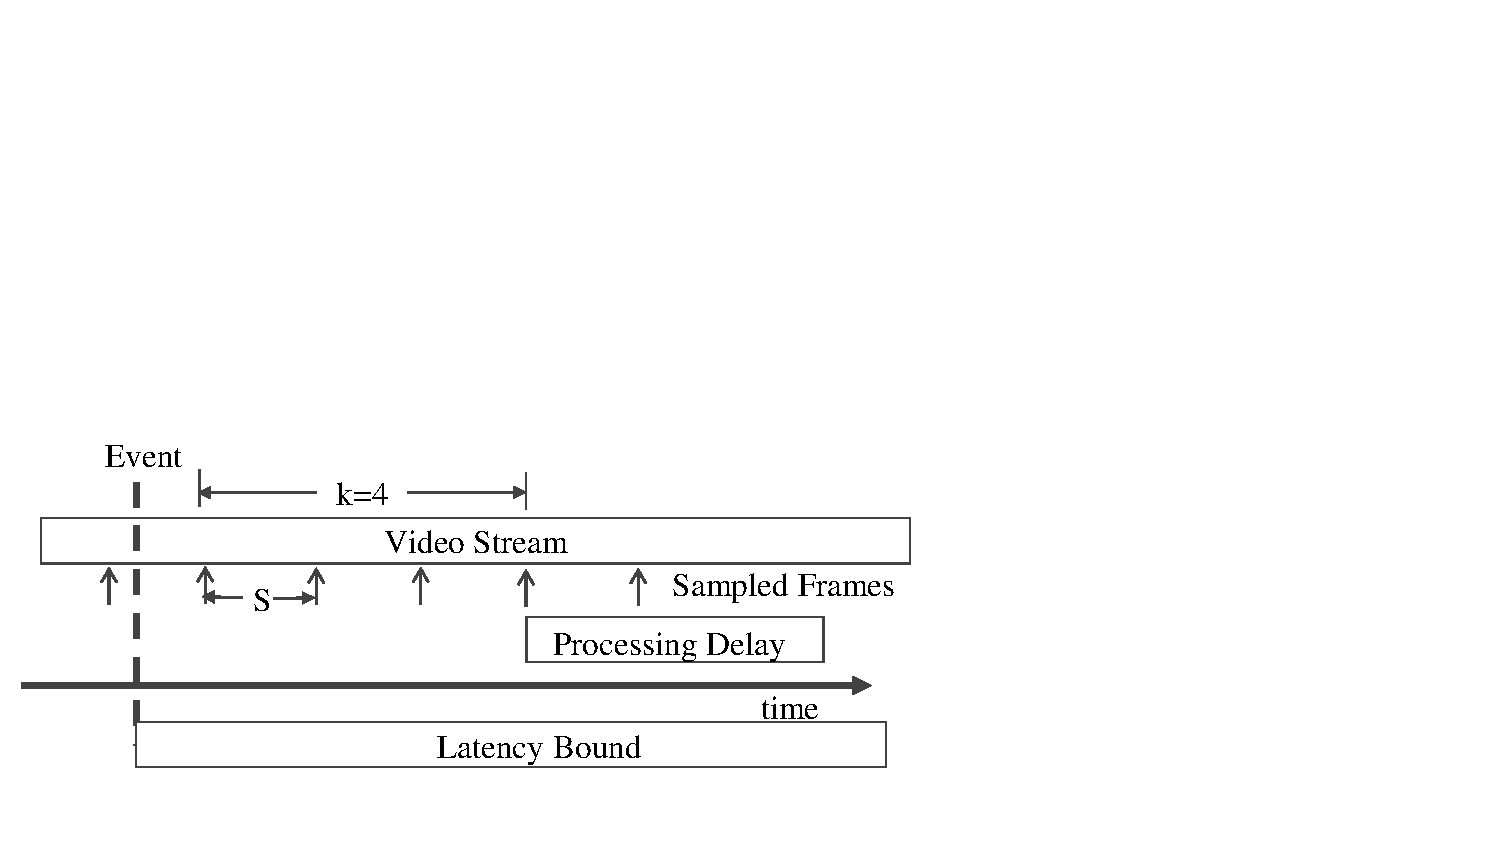
\includegraphics[width=\textwidth,trim=0em 3em 20em 15em, clip]{FIGS/fig-lego-sampling-model.pdf}
\caption{\small Dynamic Sampling Rate for LEGO}
\label{fig:lego-sampling-model}
\end{figure}

We use the LEGO application from Section~\ref{sec:example-apps} to show the
effectiveness of adaptive sampling. By default, the LEGO application runs at
active phase. The application enters passive phases immediately following the
delivery of an instruction, since the user is going to take a few seconds
searching and assembling LEGO blocks. The length and sampling rate of a passive
phase is provided by the application to the framework. We provide the following
system model as an example of what can be provided. We collect five LEGO traces
with 13739 frames as our evaluation dataset.

\textbf{Length of a Passive Phase: }
We model the time it takes to finish each step as a Gaussian distribution. We
use maximum likelihood estimation to calculate the parameters of the Guassian
model.

 
\begin{figure}
\small\centering
\begin{subfigure}{.45\linewidth}
  \centering
  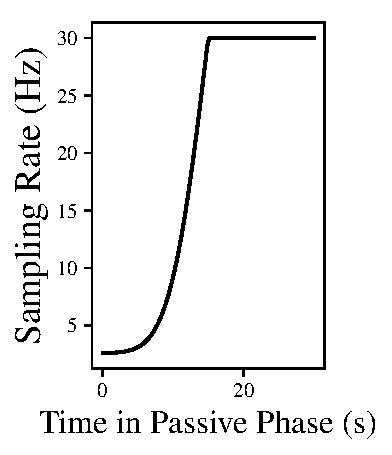
\includegraphics[width=\linewidth, trim=0em 0em 0em 0em, clip]{FIGS/fig-lego-adaptive-sr.pdf}
  {\small (a) Passive Sampling Rate}
\end{subfigure}
\begin{subfigure}{.45\linewidth}
    \centering
    \includegraphics[width=0.92\linewidth, trim=0em 0em 0em 0em, clip]{FIGS/fig-lego-example-sr.pdf}
   {\small (b) Trace Sampling Rate}
\end{subfigure}
\caption{\small Adaptive Sampling Rate}
\label{fig:adaptive-sampling-example}
\end{figure}

\textbf{Lowest Sampling Rate in Passive Phase: }
The lowest sampling rate in passive phase still needs to meet application's
latency requirement. Figure~\ref{fig:lego-sampling-model} shows the system model
to calculate the largest sampling period S that still meets the latency bound.
In particular,
$$(k-1)S + processing\_delay \leq latency\_bound $$ $k$ represents the
cumulative number of frames an event needs to be detected in order to be
certain an event actually occurred. The LEGO application empirically sets this
value to be 5. 

\textbf{Adaptation Algorithm: }
At the start of a passive phase, we set the sampling rate to the
minimum calculated above.  As time progresses, we gradually increase
the sampling rate.  The idea behind this is that the initial low
sampling rates do not provide good latency, but this is acceptable, as
the likelihood of an event is low.  As the likelihood increases (based
on the Gaussian distribution described earlier), we increase sampling
rate to decrease latency when events are likely.
Figure~\ref{fig:adaptive-sampling-example}(a) shows the sampling rate
adaptation our system employs during a passive phase.
The sampling rate is calculated as $$sr = \\
%
 min\_sr + \alpha * (max\_sr - min\_sr) * cdf\_Gaussian(t)$$ 
%
$sr$ is the sampling rate. $t$ is the time after an instruction has been given. $\alpha$ is
a recovery factor which determines how quickly the sampling rate
rebounds to active phase rate. 


Figure~\ref{fig:adaptive-sampling-example}(b) shows the sampling rate
for a trace as the application runs. The video captures a user doing 7
steps of a LEGO assembly task. Each drop in sampling rate happens
after an instruction has been delivered to the user.
Table~\ref{tab:adaptive-sample-eval} shows the percentage of frames
sampled and guidance latency comparing adaptive sampling with naive
sampling at half frequency. Our adaptive sampling scheme requires
processing fewer frames while achieving a lower guidance latency.

\begin{table}[]
\small\centering
\begin{tabular}{|c|c|c|}
\hline
Trace  & \begin{tabular}[c]{@{}c@{}}Sample\\ Half Freq\end{tabular} & \begin{tabular}[c]{@{}c@{}}Adaptive\\ Sampling\end{tabular} \\ \hline
1 & 50\%          & 25\%              \\ \hline
2 & 50\%          & 28\%              \\ \hline
3 & 50\%          & 30\%              \\ \hline
4 & 50\%          & 30\%              \\ \hline
5 & 50\%          & 43\%              \\ \hline
\end{tabular}\\[0.1in]
{\small (a) Percentage of Frames Sampled}\\[0.2in]

\begin{tabular}{|c|c|}
\hline
                                                            & \begin{tabular}[c]{@{}c@{}}Guidance Delay \\ (frames$\pm$stddev)\end{tabular}
                                                            \\ \hline
\begin{tabular}[c]{@{}c@{}}Sample Half Freq\end{tabular}      & 7.6 $\pm$ 6.9                                                                  \\ \hline
\begin{tabular}[c]{@{}c@{}}Adaptive Sampling\end{tabular} &  5.9 $\pm$ 8.2                                                                  \\ \hline
% \begin{tabular}[c]{@{}c@{}}Theoretical Minimum\end{tabular} &  ?? $$                                                                  \\ \hline
\end{tabular}\\[0.1in]
{\small (b) Guidance Latency}\\[0.1in]
\caption{\small Frames Sampled and Guidance Latency}
\label{tab:adaptive-sample-eval}
\vspace{-0.2in}
\end{table}
\section{IMU-based Approaches: Passive Phase Suppression}

% comment: add image quality evaluation?

\begin{figure}[h]
\begin{center}
\includegraphics[width=.9\linewidth]{FIGS/fig-imu-trace-lego.pdf}\\
{\small (a) LEGO}
\includegraphics[width=.9\linewidth]{FIGS/fig-imu-trace-pingpong.pdf}\\
{\small (b) PING PONG}
\end{center}
\vspace{-0.1in}
\caption{\small Accuracy of IMU-based Frame Suppression}
\label{fig:imu-trace-example}
\vspace{-0.1in}
\end{figure}

In many applications, passive phases can often be associated with the
user's head movement. We illustrate with two applications here. In
LEGO, during the passive phase, which begins after the user receives
the next instruction, a user typically turns away from the LEGO board
and starts searching for the next brick to use in a parts box. During
this period, the computer vision algorithm would detect no meaningful
task states if the frames are transmitted.  In PING PONG, an active
phase lasts throughout a rally.  Passive phases are in between actual
game play, when the user takes a drink, switches sides, or, most
commonly, tracks down and picks up a wayward ball from the floor.
These are associated with much large range of head movements than
during a rally when the player generally looks toward the opposing
player.  Again, the frames can be suppressed on the client to reduce
wireless transmission and load on the cloudlet.  In both scenarios,
significant body movement can be detected through Inertial Measurement
Unit (IMU) readings on the wearable device, and used to predict those
passive phases.

For each frame, we get a six-dimensional reading from the IMU:
rotation in three axes, and acceleration in three axes.  We train an
application-specific SVM to predict active/passive phases based on IMU
readings, and suppress predicted passive frames on the client.
Figure~\ref{fig:imu-trace-example}(a) and (b) show an example trace
from LEGO and PING PONG, respectively.  Human-labeled ground truth
indicating passive and active phases is shown in blue.  The red dots
indicate predictions of passive phase frames based on the IMU
readings; these frames are suppressed at the client and not
transmitted.  Note that in both traces, the suppressed frames also
form streaks. In other words, a number of frames in a row can be
suppressed. As a result, the saving we gain from IMU is orthogonal to
that from adaptive sampling.

Although the IMU approach does not capture all of the passive frames
(e.g., in LEGO, the user may hold his head steady while looking for
the next part), when a passive frame is predicted, this is likely
correct (i.e., high precision, moderate recall).  Thus, we expect
little impact on event detection accuracy or latency, as few if any
active phase frames are affected.  This is confirmed in
Table~\ref{tab:imu-result}, which summarizes results for five traces
from each application.  We are able to suppress up to 49.9\% of
passive frames for LEGO and up to 38.4\% of passive frames in case of
PING PONG on the client, while having minimal impact on application
quality --- incurring no delay in state change detection in LEGO, and
less than 2\% loss of active frames in PING PONG.

\begin{table}[h]
\small\centering
\begin{tabular}{| l | c | c |}
   \hline
        & Suppressed  &  Max Delay of \\ 
        & Passive Frames (\%)   & State Change Detection \\ \hline
    Trace 1 & 17.9\%    & 0 \\
    Trace 2 & 49.9\%    & 0 \\
    Trace 3 & 27.1\%    & 0 \\
    Trace 4 & 37.0\%    & 0 \\
    Trace 5 & 34.1\%    & 0 \\
    \hline
\end{tabular}\\[0.1in]
{\small (a) LEGO}\\[0.1in]

\begin{tabular}{| l | c | c |}
    \hline
        & Suppressed        & Loss of  \\
        & Passive Frames (\%)    & Active Frames (\%) \\ \hline
    Trace 1 & 21.5\%    &   0.8\%   \\
    Trace 2 & 30.0\%    &   1.5\%   \\
    Trace 3 & 26.2\%    &   1.9\%   \\
    Trace 4 & 29.8\%    &   1.0\%   \\
    Trace 5 & 38.4\%    &   0.2\%   \\
    \hline
\end{tabular}\\[0.1in]
{\small (b) PING PONG}\\[0.1in]
\caption{\small Effectiveness of IMU-based Frame Suppression}
\label{tab:imu-result}
\end{table}

\section{Related Work}
\label{sec: workload-related}

Although edge computing is new, the techniques for reducing offered load to
adapt application behaviors examined in this chapter bear some resemblance to
work that was done in the early days of mobile computing.

Several different approaches to adapting application fidelity have been studied.
Dynamic sampling rate with various heuristics for adaptation have been tried
primarily in the context of individual mobile devices for energy
efficiency~\cite{lorincz2009mercury, lorincz2008resource, vallina2012energy,
lane2010survey}. Semantic deduplication to reduce redundant processing of frames
have been suggested by ~\cite{Hu2015, kang2017noscope, hsieh2018focus,
zhang2015design}. Similarly, previous works have looked at suppression based on
motion either from video content~\cite{naderiparizi2017glimpse,
lebeckcollaborative} or IMUs~\cite{jain2015overlay}. Others have investigated
exploiting multiple deep models with accuracy and resource
tradeoffs~\cite{han2016mcdnn,jiang2018chameleon}. In addition, using tracking as
approximate result of detection and recognition has been explored to leverage
the temporal locality of video data and reduce computational
demand~\cite{wang2017scalable, chen2015glimpse, you1999hybrid}. While most of
these efforts were in mobile-only, cloud-only, or mobile-cloud context, we
explore similar techniques in an edge-native context.


Partitioning workloads between mobile devices and the cloud have been
studied in sensor networks~\cite{newton2009wishbone},
throughput-oriented systems~\cite{cuervo2010maui, yi2017lavea}, for
interactive applications~\cite{ra2011odessa, chen2015glimpse}, and
from programming model perspectives~\cite{balan2003tactics}. We believe
that these approaches will become important techniques to scale
applications on heavily loaded cloudlets.
\chapter{Cloudlet Resource Management for Graceful Degradation of Service}
{\em Elasticity} is a key attribute of cloud computing.  When load
rises, new servers can be rapidly spun up.  When load subsides, idle
servers can be quiesced to save energy.  Elasticity is vital to
scalability, because it ensures acceptable response times under a wide
range of operating conditions.  To benefit, cloud services need to be
architected to easily scale out to more servers.  Such a design is
said to be ``cloud-native.''

In contrast, edge computing has limited elasticity.  As its name
implies, a cloudlet is designed for much smaller physical space and
electrical power than a cloud data center.  Hence, the sudden arrival
of an unexpected flash crowd can overwhelm a cloudlet and its wireless
network.  Since low end-to-end latency is a prime reason for edge
computing, shifting load elsewhere (e.g., the cloud) is not an
attractive solution.  {\em How do we build multi-user edge computing
  systems that preserve low latency even as load increases?}  That is
our focus.

\begin{figure*}
\begin{minipage}[b]{4.3in}
\begin{minipage}[c]{1.68in}
\includegraphics[scale=0.3]{FIGS/fig-3tier-A.pdf}
\end{minipage}
\begin{minipage}[c]{1.75in}
\vspace{0.01in}
\includegraphics[scale=0.16]{FIGS/fig-3tier-B-cropped.pdf}\\
\end{minipage}
\begin{minipage}[c]{0.55in}
\includegraphics[scale=0.33]{FIGS/fig-3tier-C.pdf}
\end{minipage}
\begin{captiontext}
  From left to right, this tiered model represents a hierarchy of
  increasing physical size, compute power, energy usage, and
  elasticity. Tier-3 represents IoT and mobile devices; Tier-2
  represents cloudlets; and Tier-1 represents the cloud.  We use
  ``Tier-2'' and ``cloudlet'' interchangeably in the paper.  We also
  use ``Tier-3'' to mean ``mobile or IoT device.''
\end{captiontext}
\vspace{-0.1in}
\caption{\small Tiered Model of Computing}
\label{fig:3tier}
\end{minipage}
\hspace*{0.1in}
\end{figure*}

Our approach to scalability is driven by the following observation.
Since compute resources and wireless capacity at the edge cannot be
increased on demand, the only paths to scalability are (a) to reduce
offered load, or (b) to reduce queueing delays through improved
end-to-end scheduling.  Otherwise, the mismatch between resource
availability and offered load will lead to increased queueing delays
and hence increased end-to-end latency.  Both paths require the
average burden placed by each user on the cloudlet and the wireless
channel to fall as the number of users increases.  This, in turn,
implies {\em adaptive application behavior} based on guidance received
from the cloudlet or inferred by the user's mobile device.  In the
context of Figure~\ref{fig:3tier}, scalability at the left is achieved
very differently from scalability at the right.  The relationship
between Tier-3 and Tier-2 is {\em non-workload-conserving}, while that
between Tier-1 and other tiers is workload-conserving.

With rare exceptions, reducing offered load is only possible with
application assistance.  Scalability at the edge is thus only
achievable for applications that have been designed with this goal in
mind.  We refer to applications that are specifically written for edge
computing as {\em edge-native applications.}  These applications are
deeply dependent on services that are only available at the edge (such
as low-latency offloading of compute, or real-time access to video
streams from edge-located cameras), and are written to adapt to
scalability-relevant guidance.  For example, an application at Tier-3
may be written to offload object recognition in a video frame to
Tier-2, but it may also be prepared for the return code to indicate
that a less accurate (and hence less compute-intensive) algorithm than
normal was used because Tier-2 is heavily loaded.  Alternatively,
Tier-2 or Tier-3 may determine that the wireless channel is congested;
based on this guidance, Tier-3 may reduce offered load by
preprocessing a video frame and using the result to decide whether it
is worthwhile to offload further processing of that frame to the
cloudlet.  In earlier work~\cite{Hu2015}, we have shown that even
modest computation at Tier-3 can make surprisingly good predictions
about whether a specific use of Tier-2 is likely to be worthwhile.

Edge-native applications may also use {\em cross-layer adaptation
  strategies,} by which knowledge from Tier-3 or Tier-2 is used in the
management of the wireless channel between them.  For example, an
assistive augmented reality (AR) application that verbally guides a
visually-impaired person may be competing for the wireless channel and
cloudlet resources with a group of AR gamers.  In an overload
situation, one may wish to favor the assistive application over the
gamers.  This knowledge can be used by the cloudlet operating system
to preferentially schedule the more important workload.  It can also
be used for prioritizing network traffic by using {\em fine-grain
  network slicing,} as envisioned in 5G~\cite{Contreras2018}.

Since the techniques for reducing offered workload are application-specific, we
focus on a specific class of edge-native applications to validate our ideas.
Our choice is a class of applications called {\em Wearable Cognitive Assistance}
(WCA) applications~\cite{ha2014towards}.  They are perceived to be ``killer apps'' for
edge computing because (a) they transmit large volumes of video data to the
cloudlet; (b) they have stringent end-to-end latency requirements; and (c) they
make substantial compute demands of the cloudlet, often requiring high-end GPUs.

We leverage unique characteristics of WCA applications to reduce
offered load through graceful degradation and improved resource
allocation.  Our contributions are as follows:
\begin{smitemize}
  \item{An architectural framework for WCA that enables graceful degradation under heavy load.}
  \item{An adaptation taxonomy of WCA applications, and techniques for workload reduction.}
  \item{A cloudlet resource allocation scheme based on degradation heuristics and external policies.}
  \item{A prototype implementation of the above.}
  \item{Experimental results showing up to 40\% reduction in offered load and graceful degradation in oversubscribed edge systems.}
\end{smitemize}


\section{System Model and Application Profiles}

% A complementary method to improve scalability is through judicious
% allocation of cloudlet resources among concurrent application
% services. 

Resource allocation has been well explored in many contexts
of computer systems, including operating system, networks, real-time
systems, and cloud data centers.  While these prior efforts can
provide design blueprints for cloudlet resource allocation, the
characteristics of edge-native applications emphasize unique design
challenges.

The ultra-low application latency requirements of edge-native
applications are at odds with large queues often used to maintain high
resource utilization of scarce resources.  Even buffering a small
number of requests may result in end-to-end latencies that are several
multiples of processing delays, hence exceeding acceptable latency
thresholds.  On the other hand, when using short queues, accurate
estimations of throughput, processing, and networking delay are vital
to enable efficient use of cloudlet resources.  However, sophisticated
computer vision processing represents a highly variable computational
workload, even on a single stream. For example, as shown in
Figure~\ref{fig:lego-dag}, the processing pipeline for LEGO has many
exits, resulting in highly variable execution times.

\begin{figure}
\centering
\includegraphics[width=\linewidth, trim=0em 30em 20em 0em,clip]{FIGS/fig-lego-dag.pdf}
\caption{LEGO Processing DAG}
\label{fig:lego-dag}
\end{figure}

To adequately provision resources for an application, one approach is
to leave the burden to developers, asking them to specify and reserve
a static amount of cores and memories needed for the service. However,
this method is known to be highly inaccurate and typically leads to
over-reservation in data-centers. For cloudlets, which are more
resource constrained, such over-reservation will lead to even worse
under-utilization or inequitable sharing of the available resources.
Instead, we seek to create an automated resource allocation system
that leverages knowledge of the application requirements and minimizes
developer effort.  To this end, we ask developers to provide target
Quality of Service (QoS) metrics or a utility function that relates a
single, easily-quantified metric (such as latency) to the quality of
user experience.  Building on this information, we construct offline
application profiles that map multidimensional resource allocations to
application QoS metrics.  At runtime, we calculate a resource
allocation plan to maximize a system-wide metric (e.g., total utility,
fairness) specified by cloudlet owner. We choose to consider the
allocation problem per application rather than per client in order to
leverage statistical multiplexing among clients and multi-user
optimizations (e.g., cache sharing) in an application.

\begin{figure}
\centering
\includegraphics[width=0.5\linewidth]{FIGS/fig-allocation-system-model-cropped.pdf}
\begin{captiontext}Only request flow is shown.\end{captiontext}
\caption{Resource Allocation System Model}
\label{fig:allocation-system-model}
\vspace{-0.2in}
\end{figure}

\subsection{System Model}
Figure~\ref{fig:allocation-system-model} shows the system model we consider.
Each application is given a separate input queue. Each queue can feed one or
more application instances, which are the units of application logic that can be
replicated (e.g. a single process or several collaborative processes). Each
application instance is encapsulated in a container with controlled resources.
In this model, with adequate computational resources, clients of different
applications have minimal sharing and mainly contend for the wireless network.

We use a utility-based approach to measure and compare system-wide
performance under different allocation schemes. For WCA, the utility
of a cloudlet response depends on both the quality of response and its
QoS characteristics (e.g., end-to-end latency). The total utility of a
system is the sum of all individual utilities. A common limitation of
a utility-based approach is the difficulty of creating these
functions. One way to ease such burden is to position an application
in the taxonomy described in Section~\ref{sec:taxonomy} and borrow
from similar applications. Another way is to calculate or measure
application latency bounds, such as through literature review or
physics-based calculation as done in~\cite{chen2017empirical}.

The system-wide performance is a function of the following independent
variables. 
\begin{enumerate}[label=(\alph*)]
    \item the number of applications and the number of clients of
each application;
    \item the number of instances of each application;
    \item the resource allocation for each instance;
\end{enumerate}

Although (a) is not under our control, Gabriel is free to adapt (b) and (c).
Furthermore, to optimize system performance, it may sacrifice the performance of
certain applications in favor of others. Alternatively, it may choose not to run
certain applications.


\begin{figure}
\centering
\begin{minipage}[b]{.35\linewidth}
\centering
\includegraphics[width=\linewidth,trim=0em 0em 0em 0em, clip]{FIGS/fig-lat-util-face.pdf}
{(a) Utility For FACE}
\end{minipage}
\begin{minipage}[b]{.6\linewidth}
\centering
\includegraphics[width=\linewidth, trim=0em 0em 0em 0em, clip]{FIGS/fig-app-profile-face.pdf}
{(b) Profile for FACE}
\end{minipage}
\caption{FACE Application Utility and Profile}
\label{fig:face-utility-and-profile}
\end{figure}

\begin{figure}
\centering
\begin{minipage}[b]{.35\linewidth}
\centering
\includegraphics[width=\linewidth,trim=0em 0em 0em 0em, clip]{FIGS/fig-lat-util-pool.pdf}
{(a) Utility For POOL}
\end{minipage}
\begin{minipage}[b]{.6\linewidth}
\centering
\includegraphics[width=\linewidth, trim=0em 0em 0em 0em, clip]{FIGS/fig-app-profile-pool.pdf}
{(b) Profile for POOL}
\end{minipage}
\caption{POOL Application Utility and Profile}
\label{fig:pool-utility-and-profile}
\end{figure}

\subsection{Application Utility and Profiles}

We build application profiles offline in order to estimate latency and
throughput at runtime. First, we ask developers to provide a utility
function that maps QoS metrics to application experience.
Figure~\ref{fig:face-utility-and-profile}(a) and
Figure~\ref{fig:pool-utility-and-profile}(a) show utility functions
for two applications based on latency bounds identified
by~\cite{chen2017empirical} for each request. Next, we profile an application
instance by running it under a discrete set of cpu and memory
limitations, with a large number of input requests. We record the
processing latency and throughput, and calculate the system-wide
utility per unit time. We interpolate between acquired data points of
(system utility, resources) to produce continuous functions.  Hence,
we effectively generate a multidimensional resource to utility profile
for each application.

We make a few simplifying assumptions to ensure profile generation and
allocation of resources by utility are tractable.  First, we assume utility
values across different applications are comparable. Furthermore, we assume
utility is received on a per-frame basis, with values that are normalized
between 0 and 1.  Each frame that is sent, accurately processed, and replied
within its latency bound receives 1, so a client running at 30 FPS under ideal
conditions can receive a maximum utility of 30 per second.  This clearly ignores
variable utility of processing particular frames (e.g., differences between
active and passive phases), but simplifies construction of profiles and modeling
for resource allocation; we leave the complexities of variable utility to future
work. Figure~\ref{fig:face-utility-and-profile}(b) and
Figure~\ref{fig:pool-utility-and-profile}(b) show the generated application
profiles for FACE and POOL. We see that POOL is more efficient than FACE in
using per unit resource to produce utility. If an application needs to deliver
higher utility than a single instance can, our framework will automatically
launch more instances of it on the cloudlet.

\section{Profiling-based Resource Allocation}
\label{sec: resource-allocation}

Given a workload of concurrent applications running on a cloudlet, and the
number of clients requesting service from each application, our resource
allocator determines how many instances to launch and how much resource (CPU
cores, memory, etc.) to allocate for each application instance.  We assume
queueing delays are limited by the token mechanism used in Original Gabriel,
which limits the number of outstanding requests on a per-client basis.


\subsection{Maximizing Overall System Utility}

As described earlier, for each application $a \in $ \{FACE, LEGO, PING PONG, POOL, \ldots \}, 
we construct a resource to utility mapping
$u_a: \mathbf{r} \rightarrow \mathbb{R}$ for one instance of the application on cloudlet, 
where $\mathbf{r}$ is a resource vector of allocated CPU, memory, etc. We formulate the 
following optimization problem which maximizes the system-wide total utility,
subject to a tunable maximum per-client limit:

\begin{equation}
  \begin{aligned}
  \max_{\{k_a, \mathbf{r}_a\}} \quad & \sum_a{k_a \cdot u_a(\mathbf{r}_a)} \\
  \textrm{s.t.} \quad & \sum_a k_a \cdot \mathbf{r}_a \preccurlyeq \hat{\mathbf{r}} \\
      & 0 \preccurlyeq \mathbf{r}_a  \quad \forall a \\
      & k_a \cdot u_a(\mathbf{r}_a) \le \gamma \cdot c_a \quad \forall a \\
      & k_a \in \mathbb{Z}
  \end{aligned}
  \end{equation}

In above, $c_a$ is the number of mobile clients requesting service from application $a$.
The total resource vector of the cloudlet is  $\hat{\mathbf{r}}$. 
 For each application $a$, we determine how many instances to launch --- $k_a$, and 
allocate resource vector $\mathbf{r}_a$ to each of them.
A tunable knob $\gamma$ regulates the maximum utility allotted 
per application, and serves to enforce a form of partial fairness (no application
can be given excessive utility, though some may still receive none). 
The larger $\gamma$ is, the more aggressive our scheduling algorithm
will be in maximizing global utility and
suppressing low-utility applications. 
%In our system model, the maximum $\gamma$ is 30 for
%clients at 30 FPS. 
By default, we set $\gamma=10$, which, based on our definition of
utility, roughly means resources will be allocated so 
no more than one third of frames (from a 30FPS source) 
will be processed within satisfactory latency bounds for a given
client.

Solving the above optimization problem is computationally difficult. We thus use an
iterative greedy allocation algorithm as follows.

\begin{algorithm}[H]
\SetAlgoLined
% \KwResult{Write here the result }
 Profile applications under varying resources\;
 $u_a(\mathbf{r})$: resource $\mathbf{r}$ to utility mapping for application
 $a$\;
\For{each application}{
  find the highest \emph{utility-to-resource} ratio $\frac{u_a(\mathbf{r})}{|\mathbf{r}|}$\;
}
 \While{leftover system resource}{
 Find the application with the largest \emph{utility-to-resource}
 $\frac{u_a(\mathbf{r}^*_a)}{|\mathbf{r}^*_a|}$, which has not been allocated
 resources\;
Allocate $k_a$ application instances,
each with resource $\mathbf{r}^*_a$, such that $k_a$ is the largest integer with
$k_a \cdot u_a(\mathbf{r}^*_a) \le \gamma \cdot c_a$\;
 }
 \caption{Iterative Allocation Algorithm to Maximize Overall System Utility}
\end{algorithm}

% For each application profile $u_a(\mathbf{r})$, we find the resource point that gives
% the highest $\frac{u_a(\mathbf{r})}{|\mathbf{r}|}$, i.e., \emph{utility-to-resource} ratio. 
% Denote this point as $\mathbf{r}^*_a$. We start with the application with the largest 
% $\frac{u_a(\mathbf{r}^*_a)}{|\mathbf{r}^*_a|}$. We allocate $k_a$ application instances,
% each with resource $\mathbf{r}^*_a$, such that $k_a$ is the largest integer with
% $k_a \cdot u_a(\mathbf{r}^*_a) \le \gamma \cdot c_a$. 
% If there is leftover resource, we move to the application with the next highest 
% utility-to-resource ratio and repeat the process.

In our implementation, we exploit the \texttt{cpu-shares} and
\texttt{memory-reservation} control options of Linux Docker containers. It puts
a soft limit on containers' resource utilization only when they are in
contention, but allows them to use as much left-over resource as needed.
\section{Evaluation}

We use five WCA applications, including FACE, PING PONG, LEGO, POOL, and IKEA
for evaluation~\cite{chen2017empirical,chen2018application}. These
applications are selected based on their distinct requirements and
characteristics to represent the variety of WCA apps. IKEA and LEGO assist users
step by step to assemble an IKEA lamp or a LEGO model. While their 2.7-second
loose latency bound is less stringent than other apps, the significance of their
instructions is high, as a user could not proceed without the instruction. On
the other hand, users could still continue their tasks without the instructions
from FACE, POOL, and PING PONG assistants. For POOL and PING PONG, the speed of
an instruction is paramount to its usefulness. For example, any instruction that
comes 105ms after a user action for POOL is no longer of value, because it is
too late to guide the next action.

\begin{figure}
  \centering
  \includegraphics[width=\linewidth, trim=0em 3em 0em 3em, clip]{FIGS/fig-sec6-reduction-legend.pdf}
  \begin{minipage}[b]{0.38\linewidth}
    \centering
    \includegraphics[height=2.5in, trim=0em 1em 0em 0em, clip]{FIGS/fig-sec6-reduction-Pingpong.pdf}\\
    {(a) PING PONG}
  \end{minipage}
  \begin{minipage}[b]{0.3\linewidth}
    \centering
    \includegraphics[height=2.5in, trim=0em 1em 0em 0em, clip]{FIGS/fig-sec6-reduction-Lego.pdf}\\
    {(b) LEGO}
  \end{minipage}
  \begin{minipage}[b]{0.3\linewidth}
    \centering
    \includegraphics[height=2.5in, trim=0em 1em 0em 0em, clip]{FIGS/fig-sec6-reduction-Pool.pdf}\\
    {(c) POOL}
  \end{minipage}
  \caption{Effects of Workload Reduction}
  \label{figs:workload-reduction}
\end{figure}


\subsection{Effectiveness of Workload Reduction}

We first evaluate the effectiveness of all of the workload reduction techniques
explored in Chapter~\ref{chapter: load}. For this set of experiments, we do not
use multiple concurrent applications. Adaptation-centric cloudlet resource
allocation is not enabled for a controlled setup. We use four Nexus 6 mobile
phones as clients. They offload computation to a cloudlet over Wi-Fi links. We
run PING PONG, LEGO, and POOL applications one at a time with 2, 4, 6, and 8
cores on the edge server. We constrain the number of cores available using Linux
cgroup. Figure~\ref{figs:workload-reduction} shows the total number of frames
processed with and without workload reduction. The yellow lines for Original
Gabriel do not have workload reduction while the blue lines for Scalable Gabriel
do. The solid lines represent the total number of frames offloaded. The dashed
lines represent the number of active frames, those frames that actually contain
user state information. Note that although the offered work is greatly reduced,
the processed frames for active phases of the application have not been
affected. Thus, we confirm that we can significantly reduce cloudlet load
without affecting the critical processing needed by these applications.

\begin{table}[]
  \centering
  \begin{tabular}{|c|c||c|c|c|c|c|}
    \hline
    Exp & \multicolumn{6}{|c|}{Number of Clients}                                    \\
    \cline{2-7}
    \#  & Total                                   & FACE & LEGO & POOL & PING & IKEA \\
        &                                         &      &      &      & PONG &      \\ \hline
    1   & 15                                      & 3    & 3    & 3    & 3    & 3    \\ \hline
    2   & 20                                      & 4    & 4    & 4    & 4    & 4    \\ \hline
    3   & 23                                      & 5    & 5    & 4    & 4    & 5    \\ \hline
    4   & 25                                      & 5    & 5    & 5    & 5    & 5    \\ \hline
    5   & 27                                      & 5    & 6    & 6    & 5    & 5    \\ \hline
    6   & 30                                      & 5    & 7    & 6    & 6    & 6    \\ \hline
    7   & 32                                      & 5    & 7    & 7    & 7    & 6    \\ \hline
    8   & 40                                      & 8    & 8    & 8    & 8    & 8    \\ \hline
  \end{tabular}
  \vspace{0.1in}
  \caption{Resource Allocation Experiment Setup}
  \label{tab:alloc-exps}
\end{table}

\subsection{Effectiveness of Resource Allocation}

We next evaluate our adaptation-centric resource allocation mechanism on a
server machine with 2 Intel{\textregistered} Xeon{\textregistered} E5-2699 v3
processors, totaling 36 physical cores running at 2.3 Ghz (turbo boost disabled)
and 128 GB memory. We dedicate 8 physical cores (16 Intel{\textregistered} hyper
threads) and 16 GB memory as cloudlet resources using cgroup. We run 8
experiments with increasing numbers of clients across four concurrent
applications. The total number of clients gradually increases from 15 to 40.
Table~\ref{tab:alloc-exps} shows the breakdown of the number of clients used for
each experiment. Note that these clients are running simultaneously, resulting
in heavier and heavier contention. We generate application adapation profiles
offline using the method discussed in Section~\ref{sec: resource-allocation}. We
leverage these profiles to optimize for maximizing the total system utility.
Figure~\ref{fig:alloc-max-util} shows how the total system utility changes as we
add more clients and hence more workload. The yellow line represents the
Original Gabriel which relies on the operating system alone to divide system
resources. The blue line shows our Scalable Gabriel approach. In the beginning,
while the system is under-utilized, we see that the Original Gabriel yields
slightly higher total utility. However, as contention increases, Original
Gabriel's total utility quickly drops, eventually more than 40\%, since every
client contends for resources in an uncontrolled fashion.  All applications
suffer, but the effects of increasing latencies are vastly different among
different applications. In contrast, scalable Gabriel maintains a high level of
system-wide utility by differentially allocating resources to different
applications based on their sensitivity captured in the adaptation profiles.

\begin{figure}[h]
  \centering
  \includegraphics[width=.9\linewidth]{FIGS/fig-alloc-max-util.pdf}
  \caption{Total Utility with Increasing Contention}
  \label{fig:alloc-max-util}
\end{figure}


Figure~\ref{fig:alloc-latency} and Figure~\ref{fig:alloc-fps} provide insights
into how scalable Gabriel strikes the balance. We present both application
throughput in terms of average frames per second and latency in terms of
90\%-tile response delay. Latencies are better controlled as resources are
dedicated to applications with high utility, and more clients are kept within
their latency bounds. Of course, with higher contention, fewer frames per second
can be processed for each client. Original Gabriel degrades applications in an
undifferentiated fashion. Scalable Gabriel, in contrast, tries to maintain
higher throughput for some applications at the expense of the others, e.g. LEGO
up to 27 clients. The accuracies of application profiles influence how well
Scalable Gabriel can manage latency. Run-time resource demand could deviate
from profiles due to the differences in the request content (e.g. image
content). Profile inaccuracies result in the overshoot of POOL and IKEA
90\%-tile latencies in Figure~\ref{fig:alloc-latency}, as the profiles
underestimate their resource demand and overestimate LEGO resource demand when
the number of clients is low. When the system becomes more crowded, the
throttling of LEGO throughput reduces such an effect.

\begin{figure}[]
  \begin{center}
    \includegraphics[width=\linewidth]{FIGS/fig-alloc-latency-legend.pdf}
    \includegraphics[width=\linewidth]{FIGS/fig-alloc-latency-baseline.pdf}
    {(a) Original Gabriel}
    \includegraphics[width=\linewidth]{FIGS/fig-alloc-latency-cpushares.pdf}
    {(b) Scalable Gabriel}
  \end{center}
  \begin{captiontext}
    \centering
    The normalization is  by per-application tight and loose
    bounds~\cite{chen2017empirical}.

    The allocation policy is to maximize the overall system utility.
  \end{captiontext}
  \caption{Normalized 90\%-tile Response Latency}
  \label{fig:alloc-latency}
\end{figure}

\begin{figure}[]
  \begin{center}
    \includegraphics[width=.9\linewidth]{FIGS/fig-alloc-latency-legend.pdf}
    \includegraphics[width=\linewidth]{FIGS/fig-alloc-fps-baseline.pdf}
    {(a) Original Gabriel}
    \includegraphics[width=\linewidth]{FIGS/fig-alloc-fps-cpushares.pdf}
    {(b) Scalable Gabriel}
  \end{center}
  \caption{Average Processed Frames Per Second Per Client}
  \label{fig:alloc-fps}
\end{figure}


\subsection{Effects on Guidance Latency}

We next evaluate the combined effects of workload reduction and
resource allocation in our system. We emulate many users running
multiple applications simultaneously. All users share the same
cloudlet with 8 physical cores and 16 GB memory. We conduct three experiments,
with 20 (4 clients per app), 30 (6 clients per app), and 40 (8 clients
per app) clients. Each client loops through pre-recorded video traces
with random starting points.  Figure~\ref{fig:frame-latency} and
Fig~\ref{fig:frame-fps} show per client frame latency and FPS
achieved. The first thing to notice is that concurrently utilizing
both sets of techniques does not cause conflicts. In fact, they appear
to be complementary and latencies remain in better control than using
resource allocation alone.

\begin{figure}[]
  \begin{center}
    \includegraphics[width=\linewidth]{FIGS/fig-alloc-latency-legend.pdf}

    \begin{tabular}{c@{}c}
      \includegraphics[width=.5\linewidth]{FIGS/fig-eval-latency-baseline.pdf}
                              & \includegraphics[width=.5\linewidth]{FIGS/fig-eval-latency-cpushares.pdf} \\
      {(a) Original  Gabriel} & {(b) Scalable Gabriel}
    \end{tabular}
  \end{center}

  \begin{captiontext}
    \centering
    The normalization is by per-application tight and loose
    bounds~\cite{chen2017empirical}.
  \end{captiontext}
  \vspace{-0.1in}
  \caption{Normalized 90\%-tile Response Latency}
  \label{fig:frame-latency}
\end{figure}

\begin{figure}[]
  \begin{center}
    % \includegraphics[width=\linewidth]{FIGS/fig-alloc-latency-legend.pdf}
    \begin{tabular}{c@{}c}
      \includegraphics[width=.5\linewidth]{FIGS/fig-eval-fps-baseline.pdf}
                             & \includegraphics[width=.5\linewidth]{FIGS/fig-eval-fps-cpushares.pdf} \\
      {(a) Original Gabriel} & {(b) Scalable Gabriel}
    \end{tabular}
  \end{center}
  \caption{Processed Frames Per Second Per Application}
  \label{fig:frame-fps}
\end{figure}

\begin{figure}[]
  \begin{center}
    \includegraphics[width=.7\linewidth]{FIGS/fig-alloc-latency-legend.pdf}
    \includegraphics[width=.7\linewidth]{FIGS/fig-sec6-latency-allocation.pdf}
  \end{center}
  \vspace{-0.1in}
  \caption{Fraction of Cloudlet Processing Allocated}
  \label{figs:resource-allocated}
\end{figure}

\begin{figure}[]
  \centering
  \includegraphics[width=0.5\linewidth, trim=0em 0em 0em 0em, clip]{FIGS/fig-sec6-latency-legend.pdf} \\
  \centering
  \begin{turn}{90}{\hspace{0.6in}\small (a) FACE}\end{turn}\hspace{0.2in}\includegraphics[width=2.5in, trim=0em 0em 0em 0em, clip]{FIGS/fig-sec6-latency-face.pdf}
  \begin{turn}{90}{\hspace{0.6in}\small (b)
      LEGO}\end{turn}\hspace{0.2in}\includegraphics[width=2.5in, trim=0em 0em 0em 0em,
    clip]{FIGS/fig-sec6-latency-lego.pdf}\\[0.08in]
  \vspace{0in}
  \begin{turn}{90}{\hspace{0.6in}\small (c) PING PONG}\end{turn}\hspace{0.2in}\includegraphics[width=2.5in, trim=0em 0em 0em 0em, clip]{FIGS/fig-sec6-latency-pingpong.pdf}
  \begin{turn}{90}{\hspace{0.6in}\small (d)
      POOL}\end{turn}\hspace{0.2in}\includegraphics[width=2.5in, trim=0em 0em 0em 0em,
    clip]{FIGS/fig-sec6-latency-pool.pdf}\\[0.08in]
  \vspace{0in}
  \begin{turn}{90}{\hspace{0.6in}\small (e) IKEA}\end{turn}\hspace{0.2in}\includegraphics[width=2.5in, trim=0em 0em 0em 0em, clip]{FIGS/fig-sec6-latency-ikea.pdf}
  \caption{Guidance Latency Compared to Loose Latency Bound}
  \label{figs:inst-delay}
\end{figure}

The previous plots consider per request latencies. The ultimate goal of our work
is to maintain user experience as much as possible and degrade it gracefully
when overloaded. For WCA applications, the key measure of user experience is
guidance latency, the time between the occurrence of an event and the delivery
of corresponding guidance. Note that guidance latency is different than per
request latency, as a guidance may need not one but several frames to recognize
a user state. Figure~\ref{figs:inst-delay} shows boxplots of per-application
guidance latency for the concurrent application experiments above. The red
dotted line denotes the application-required loose bound. It is clear that our
methods control latency significantly better than the baseline. Scalable Gabriel
is able to serve at least 3x number of clients when moderately loaded while
continuing to serve more than half of the clients when severely loaded. In these
experiments, the utility is maximized at the expense of the FACE application,
which provides the least utility per resource consumed. At the highest number of
clients, scalable Gabriel sacrifices the LEGO application to maintain the
quality of service for PINGPONG and POOL. This differentiated allocation is
reflected in Figure~\ref{figs:resource-allocated}. In contrast, with original
Gabriel, none of the applications are able to regularly meet deadlines.
\section{R\lc{elated} W\lc{ork}}
\label{sec: resource-management-related}

Deadline-based scheduling algorithms and mechanisms have been studied
extensively in the literature. Many work~\cite{tokuda1990real, kao1993deadline,
    stankovic2012deadline, steiger2004operating} exist in the context of real-time
systems. Some use utility functions for scheduling tasks with soft
deadlines~\cite{ravindran2005recent, li2004utility}. While we draw
inspiration from these systems, our resource allocation focuses on application
adaptation characteristics in addition to meeting latency requirements.
Many mobile systems leverage application adaptation. Notably,
Odyssey~\cite{Noble1997} and extensions~\cite{Flinn1999} proposed upcall-based
collaboration between a mobile's operating system and its applications to adapt
to variable wireless connectivity and limited battery. Such adaption was purely
reactive by the mobile device; in our context, adaptation for a collection of
devices can be centrally managed by their cloudlet, with failover to reactive
methods as needed. Exploration of tradeoffs between application fidelity and
resource demand led to the concept of {\em multi-fidelity
        applications}~\cite{Satya1999}; such concepts are relevant to our work, but the
critical computing resources in our setting are those of the cloudlet rather
than the mobile device. More recently,
~\cite{boutin2014apollo,yao2014haste,verma2015large,ousterhout2013sparroW,delimitrou2014quasar,schwarzkopf2013omega}
study cluster scheduling in data-center context. These systems target a diverse
range of workload, take resource reservation demands, and focus on the
scalability of scheduling. In contrast, our resource allocation scheme focuses
on edge-native applications, in particular, wearable cognitive assistance, and
profile their characteristics for better outcomes in oversubscribed edge
scenarios. Closely related, dynamic resource management in the cloud for video
analytics have been explored by~\cite{sembiring2013dynamic, fu2015drs,
    kaseb2015cloud}. Some also leverage profile-based adaptation for more efficient
video analytics resource management~\cite{zhang2017live, hung2018videoedge,
    jiang2018chameleon}. However, most of these systems focus on throughput-oriented
analytics application on large clusters. In contrast, we target interactive
performance on relatively small edge deployments.



\section{C\lc{onclusion} \lc{and} F\lc{uture} W\lc{ork}}
\label{sec:conclusion}


More than a decade ago, the emergence of cloud computing led to the
realization that applications had to be written in a certain way to
take full advantage of elasticity of the cloud.  This led to the
concept of ``cloud-native applications'' whose scale-out capabilities
are well matched to the cloud, as well as tools and techniques to
easily create such applications.

The emergence of edge computing leads to another inflection point in
application design.  In particular, it leads to ``edge-native
applications'' that are deeply dependent on attributes such as low
latency or bandwidth scalability that can only be obtained at the edge.
However, as this paper has shown, edge-native applications have to be 
written in a way that is very different from cloud-native applications
if they are to be scalable.

The is the first work to show that cloud-native implementation
strategies that focus primarily on dynamic scale-out are unlikely to
be effective for scalability in edge computing.  Instead, edge-native
applications need to adapt their network and cloudlet resource demand
to system load.  As the total number of Tier-3 devices associated with
a cloudlet increases, the per-device network and cloudlet load has to
decrease.  This is a fundamental difference between cloud-native and
edge-native approaches to scalability. 

In this paper, we explore client workload reduction and server resource
allocation to manage application quality of service in the face of contention
for cloudlet resources. We demonstrate that our system is able to ensure that in
overloaded situations, a subset of users are still served with good quality of
service rather than equally sharing resources and missing latency
requirements for all.

This work serves as an initial step towards practical resource management for
edge-native applications. There are many potential directions to explore further
in this space. We have alluded to some of these earlier in the paper. One
example we briefly mentioned is dynamic partitioning of work between Tier-3 and
Tier-2 to further reduce offered load on cloudlets.  In addition, other resource
allocation policies, especially fairness-centered policies, such as max-min
fairness and static priority can be explored when optimizing overall system
performance. These fairness-focused policies could also be used to address
aggressive users, which are not considered in this paper.  While we have shown
offline profiling is effective for predicting demand and utility for WCA
applications, for a broader range of edge-native applications, with ever more
aggressive and variable offload management, online estimation may prove to be
necessary. Another area worth exploring is the particular set of control and
coordination mechanisms to allow cloudlets to manage client offered load
directly. Finally, the implementation to date only contains allocation of
resources but allows the cloudlet operating system to arbitrarily schedule
application processes.  Whether fine-grained control of application scheduling
on cloudlets can help scale services remains an open question.


% \section{Evaluation of Cloudlet Resource Management}
% \section{End-to-End Evaluation of Resource Management}
% \chapter{Wearable Cognitive Assistance Development Tools}
\label{chapter: app-dev}

While previous chapters address the system challenges of scaling wearable
cognitive assistance at the edge, another key obstacle to the widespread
adoption of WCAs is the level of specialized skills and the long development
time needed to create new applications. Such expertise include task domain
knowledge, networked application development, and computer vision.
Researchers~\cite{chen2018application} report that it typically takes multiple
person-months of effort to create a single application. The majority of
development time is spent on learning new computer vision techniques, selecting
robust algorithms to use through trial and error, and implementing the
application. The high barrier of entry significantly limit the number of
wearable cognitive assistants available today. This is clearly not scalable. 

In this chapter, we reflect on existing ad hoc WCA development process, propose
a new development methodology centered around DNN-based object detection, and
introduce development tools to lower the barrier of WCA development. Our goal is
to simplify the process so that a small team (1-2 people) of a task expert and a
developer, without computer vision expertise, can create an initial version of a
Gabriel application within a few days. This is a productivity improvement of at
least one order of magnitude. Refinement and tuning may take longer, but can be
guided by early use of the application. 

Simplification is difficult. The application needs a precise definition of the
end point of each step (e.g., a particular screw mounted flush into a
workpiece), yet needs to be tolerant of alternative paths to reaching that end
point (e.g., hand-tightening versus using a screwdriver). We assume the small
development team has knowledge of the task specifics and general programming
skills, but not necessarily experiences with wearables and machine learning.

\section{Ad Hoc WCA Development Process}
\label{sec: app-dev-adhoc}

\begin{figure}
  \centering
  \includegraphics[trim={0 6cm 0 0},width=\linewidth]{FIGS/ad-hoc-workflow}
	\caption{Ad Hoc Development Workflow}
    \label{figs:workflow}
\end{figure}

Existing ad hoc development process of wearable cognitive assistance can be
described as figure~\ref{figs:workflow}. Developers first work with task expert
to identify and pinpoint a specific use case. With the use case in mind, the
development team need to identify essential visual states that can be reliably
recognized with machine vision. In the meantime, the use case is broken down
into individual steps. For each step, feedback to users are created based on
detected visual states. Potential errors are also enumerated and included as
additional steps. We refer to the complete set of the steps annotated with
visual states and feedback as the \textit{Task Model}. For example, for the LEGO
wearable cognitive assistance ~\cite{chen2017empirical}, the task models
contains the sequence of blocks to build up the final assembled lego piece,
together with potential misused blocks. The visual states to recognize are the
current pieces on the lego board, including the shape and the color of
individual lego block, and the composed shape.

Notably, a task model is not only determined by the task itself, but also
influenced heavily by visual states that can be reliably detected. In fact, it
is common to alter the sequence of steps or introduce additional steps to reduce
the difficulties and improve the reliability of computer vision recognition. In
fact, since there is a human in the loop, relying on humans to do what they are
good at is the main reason that wearable cognitive assistance can be implemented
without solving perception and planning problems intrinsic to robotics. For
example, a frequently used technique is to ask the user to hold the object of
interests at certain viewpoints as shown in the image guidance. Narrowing the
viewing angle makes the recognition problem more tractable.

The task model serves as a blueprint for implementation. For each step in the
task model, developers select and implement computer vision algorithms in order
to recognize the visual states. Custom logic is also written to handle step
transitions and interface with the Gabriel platform. After initial
implementation, test runs and measurements are conducted to evaluate the
robustness of computer vision checks and end-to-end application latency. The
implementation process is typically iterative to allow trials-and-errors in
choosing computer vision algorithms.

The ad hoc development process has unnecessary high requirements and burden for
WCA creators.
\begin{enumerate}
  \item They needs to be familiar with various computer vision algorithms to determine
what visual states can be recognized reliably. The knowledge of selecting
algorithms for specific scenarios often requires year of experience in
developing computer vision applications. This high bar of entry hinders more
WCA to be developed.
  \item It takes a significant amount of time to implement computer vision
algorithms for the trial-and-error workflow. Several months of coding time can
turn into a fruitless outcome when the algorithm is a bad fit. For WCAs with
tens or hundreds of visual states to be recognized, such manual implementation
is not scalable. Needed are automated methods to create visual state recognizers.
  \item The tight coupling of task model design and visual state recognition
calls for deep understanding in both task domain and computer vision. When
visual states in the task model end up being too difficult for the state-of-art
algorithms, the development team need to adjust the task model to either use
alternative methods or employing user assistance to identify the state. For
instance, in the RibLoc application, a task step is changed to asking the user
to read out a word on the gauge instead of performing optical character
recognition on the lightly-colored characters. Even worse, sometimes changes the
task workflow are needed. Therefore, close collaborations among task experts and
developers are needed due to this tight intertwinement between task model design
and computer vision algorithm exploration. Methodologies and tools that provides
quick turn-around when the task model changes can significantly reduce the
overall development time.
\end{enumerate}


% Among all the development procedures, creating the computer vision checks to
% detect user states consumes the most of development time and requires computer
% vision expertise and experience. With the adoption of DNNs, developers no longer
% need to spend days to select and tweak handcrafted features. Instead, the entire
% model is trained end-to-end using labeled data. However, DNNs, with millions of
% parameters to train, requires a significant amount of training data. Collecting
% and labeling data are time-consuming and painstaking. Besides, to craft and
% implement a DNN by hand is not trivial. Significant machine learning background
% is needed to tweak network architectures and parameters. Therefore, developer
% tools are needed to both help label the data and create deep neural networks.

% In summary, implementing the workflow of cognitive assistance takes time and
% efforts. Ad-hoc implementation requires a team of domain experts, developers and
% computer vision experts. Such development model cannot scale to thousands of
% applications. Therefore, Gabriel needs to be extended with tools to reduce the
% effort of creating wearable cognitive assistants.

% Existing ad-hoc approach to develop wearable cognitive assistance not only takes
% a long time, but also requires significant amount of computer vision expertise.
% Developers new to wearable cognitive assistance would need to spend months
% learning computer vision basics and acquire intuitions to determine what is
% achievable before developing an application. 

% Figure~\ref{fig:workflow} shows the ad-hoc development process. 

\section{A Quick Prototype Methodology}

To streamline the development process and lower the barrier of entry, we propose
a new prototype methodology centering around:
\begin{enumerate}
  \item  Use deep neural network (DNN) based object detection as the universal
  building block for visual state recognition.
  \item Use finite state machine to represent application task model.
\end{enumerate}
We first introduce the concept of this methodology and describe its benefits in
this section and then introduce tools we have built to automate this methodology
in detail in subsequent sections.

\subsection{Object as the Universal Unit to Recognize Visual State}

To replace manual selection of computer vision algorithms through trial and
error, we propose to use DNN-based object detection as the fundamental building
blocks to detect user states. Using object detection as the universal building
block means that each visual state should be decomposed and described as a
collection of individual objects along with their attributes and relationship.
We argue that objects as fundamental building blocks provide expressive and
flexible constructions that are capable of describing a wide range of visual
user states important to WCAs. Intuitively, the addition and removal of objects
from the scene is straightforward to express. Spatial relationships among
objects (e.g. close to, on the left of, overlap significantly) captures
important visual features that can be used to infer deep user states. For
example, the detection of two Ikea furniture pieces close to each other can
indicate they have been assembled together. Moreover, temporal relationships add
confidence to the inference made from spatial relationship. The detection of two
pieces of furniture close to each other in the last 30 frames implies strongly
that they have been assembled together.

\begin{figure}
  \centering
  \includegraphics[trim={0 0 0 0},width=\linewidth]{FIGS/pingpong.jpeg}
	\caption{A Frame Seen by the PING PONG Assistance}
    \label{figs:pingpong-frame}
\end{figure}

To illustrate the effectiveness of this object centered approach, we showcase
how existing applications built without this methodology in mind can be easily
expressed with objects. Figure~\ref{figs:pingpong-frame} shows an image that will
trigger the PING PONG assistance to provide an instruction to hit the ball to
the left. We can express this visual state with a collection of objects, namely
the Ping-Pong table, the ball, and the opponent. These objects needs to satisfy
the following spatial relationship for the instruction ``hit to the LEFT'' to be
generated. To improve the accuracy of our instruction, we can require the
spatial relationship of these objects to be hold true for at least two
consecutive frames before an instruction is generated.

\begin{itemize}
  \item The Ping-Pong ball is above the Ping-Pong table for an active rally.
  \item The opponent is on the right side of the Ping-Pong table.
  \item The ball is also on the right side of the Ping-Pong table.
\end{itemize}

\begin{figure}
  \centering
  \includegraphics[trim={0 0 0 0},width=\linewidth]{FIGS/lego}
	\caption{A Frame Seen by the LEGO Assistance}
    \label{fig:lego-image}
\end{figure}

Similarly, we can express the visual states using objects for another
application LEGO. Figure~\ref{fig:lego-image} shows a visual state for the
assembled pieces. Here the collection of objects needs to be present are two
blue Lego blocks, one black block, one white block, and one yellow block. The
spatial relationships among these block include:

\begin{itemize}
  \item The yellow block should be at the bottom and longer than all other blocks.
  \item The white block should be in the middle of a blue block and the yellow
  block. It should have the same width as the blue block.
  \item The black block should be on the left of a blue block and the white
  block. It should also be on the bottom of a blue block.
  \item One blue bock should be at the top of all other pieces.
\end{itemize}

One challenge with object detection is to obtain the absolute scale. In this
example, it would be difficult to get the exact width of the lego block (e.g.
whether it is a 1x4 or 1x3 lego piece) with object detection alone. However,
once the location of object is detected, additional processing can be leveraged
to identify objects' attributes. In this particular case, we can leverage the
dots on the lego board to calculate the absolute size of lego pieces.

The key benefit of using object detection as the universal unit to recognize
visual states is the possibility of automation. In recent years, deep neural
networks have dramatically increased the accuracy of object
detection~\cite{zou2019object}. In 2008, the best object detector, based on
deformable part model~\cite{felzenszwalb2008discriminatively}, achieved a mean
average precision (mAP) of 21~\% on the Pascal Visual Object Classes
dataset~\cite{everingham2010pascal}. In less than ten years, deep neural
networks~\cite{he2017mask},~\cite{Ren2015},~\cite{He2016},~\cite{lin2017focal}
have quadrupled the accuracy to be 84~\% on the same dataset. For a wide range
of real-world objects, DNNs have been shown to be effective at accurate
detection and identification in natural photographs.  They have been
demonstrated to differentiate between even subtly different classes, such as
breeds of dogs, and have been shown to approach human-level accuracies. Many
commerical products now offer object detection features using DNNs. For example,
Google Photos and Pinterest Visual Search provide users the capability to search
for images containing object of interest.

In addition to significant improvement in accuracy, DNNs also provide a unified
method to create object detectors. Modern DNN-based object detectors employ
end-to-end learning, in which one or multiple deep neural network are trained to
predict the object classes and locations directly from RGB images. Gone are the
need of hand-crafted feature engineering. Instead, DNNs find distinguishable
features on their own as they are presented with between labeled examples of
different objects. The replacement of custom CV code with machine-learned models
makes automation possible. A typical DNN training process consisted of the
following steps.

\begin{enumerate}
  \item Collect training examples of object of interests from diverse
  background, perspective, and lighting.
  \item Annotate training examples with bounding boxes and class names to create
  a dataset of training data, evaluation data, and test data.
  \item Implement a DNN-based object detection network, typically using machine learning frameworks,
  such as Tensorflow~\cite{abadi2016tensorflow} or
  PyTorch~\cite{paszke2019pytorch}.
  \item Continuously train and evaluate the DNN using the labeled dataset.
  \item Test the DNN accuracy on the test data.
\end{enumerate}

While a unified training method eliminates manual feature engineering, creating
a DNN-based object detector is still both time-consuming and painstaking for the
following reasons. First, DNNs often have millions of model parameters and
therefore requires millions of labeled examples to train from scratch.
Collecting and labeling such large amount of training data takes significant
manual labor. Second, implementing a DNN correctly for object detector is not
trivial and still require significant amount of knowledge of neural networks.
For example, state-of-art object detectors uses custom layers other than
convolutional layer for better performance. Data augmentation, batch
normalization, and drop out are needed at training time for better results in
the optimization process, but should be disabled during inference time. To
streamline the process of creating DNN-based object detectors, we provide a web
app TPOD~\ref{sec: app-dev-tpod} that hide the implementation details from the
developers and allow them to train a DNN object detector from their browser
without writing a single line of code.

\subsection{Finite State Machine (FSM) as Application Representation}

While the Gabriel platform handles data capture and transmission from mobile
wearable devices to cloudlet, application developers still need to write custom
business logic for each use case. Since the task model can change frequently
during development time, a fast turn-around time to implement changes is needed
to reduce the overall development time. Therefore, we propose a finite state
machine representation of application logic and a GUI tool in order to reduce
the development time and efforts for application logic. 

Our choice of finite state machine representation is based on the observation
that WCAs, in their nature, are finite state machines. A FSM ``State''
corresponds to a user state at a particular time. When the application is in a
particular state, it needs to run some computer vision processing to analyze the
current scene. We refer to the computer vision algorithms as ``Processors'' for
the state. The outputs of ``Processors'' are symbolic states of current scene.
For example, it can be a vector of object classes and locations. ``Transitions''
to other state happens when the symbolic states meet some criteria, for example,
the presence of a new object. We refer to these criteria as ``Predicates'' for
transitions. A ``State'' can have multiple transitions into several adjacent
``States''. Each ``Transition'' has its own ``Predicate''. ``Transitions'' also
have the concept of precedence. The first ``Transition'' whose ``Predicate'' is
satisfied will be triggered for a state change. ``Tranistions'' also have
guidance instructions associated with them. When a ``Transition'' is taken, the
corresponding guidance instruction is delivered to the user.


\begin{figure}
  \centering
  \includegraphics[trim={0 0 0 0},width=\linewidth]{FIGS/fsm-example}
	\caption{Example FSM}
    \label{figs:fsm-example}
\end{figure}

Figure~\ref{figs:fsm-example} shows an example of a simple WCA represented as a
finite state machine. This example WCA checks whether a piece of bread is
present. If so, it congratulates the user. If on the other hand it detects a
piece of ham is present. It corrects the user to replace the ham with a bread.
There are four states in total. The application starts from the ``Start'' state
and immediately transition to ``Check Bread'' state as the transition predicate
is ``Always''. At ``Check Bread'' state, for each frame, it runs its processor,
a DNN to detect bread and ham, to extract the symbolic state of the current
frame. It also iterates through its transitions to check if any of them are
satisfied. If a ``Bread'' is detected, the transition predicate to ``Finish'' is
satisfied and hence the transition taken. The corresponding instruction ``Good
Job'' is delivered to the user. Then the current state of the applcation becomes
``Finish''. Similarly, when in ``Check Bread'' state, if a ``Ham'' is detected,
the transition to ``Error: Ham'' state is satisfied and taken. The instruction
``Replace Ham with Bread'' will be delivered as the corrective guidance to the
user.

With FSM representing application logic, we impose structure on the component
and the logic of the application. We provide a python API and a web GUI,
introduced in Section~\ref{sec: app-dev-statemachine} to enable developers to
quickly create a cognitive assistant without writing custom code. 

\section{Tools For Painless Object Detection (TPOD)}
\label{sec: app-dev-tpod}

Training a DNN for object detection is not trivial.  In particular, it involves
constructing a correctly-labeled training data set with millions of positive and
negative examples. The training process itself may take days to complete, and
involves a set of arcane procedures to ensure both convergence and efficacy of
the model. Fortunately, one does not typically need to train a DNN from scratch.
Rather, one can start with a pretrained model based on a public image data set
such as ImageNet, and then adapt it to detect custom classes for a new
application, though a process called \emph{transfer learning}.  The key idea is
that much of the training teaches the model to discover low-level features, such
as edges, textures, shapes, and patterns that are useful in distinguishing
objects, and such features can largely be reused in other detection tasks on
similar images.  Thus, adapting a pretrained model for new object classes
requires only thousands of examples and hours of training time. 

However, even with transfer learning, collecting a labeled training set of a
thousand examples per object class can be a daunting and painful task. In
addition, implementing DNNs requires expertise and takes time. TPOD is a
web-based tool we developed to streamline the process of creating DNN-based
object detectors for fast prototype. It provides a tracking-assisted labeling
interface for speedy annotation and transfer learning-based DNN training and
evaluation backends that abstract the nuances of DNNs. It helps to greatly
reduce the labeling effort while constructing the dataset, and automates and
takes some of the guesswork out of training a DNN model.

% A user would first
% upload short videos of the object collected from varying lighting conditions and
% perspectives. Then, the user would label these objects using TPOD's labeling
% interface. TPOD assists labeling by tracking the labeled object across frames.
% Augmenting training data with synthetically generated data is also supported. A
% user then can start training from the web interface. TPOD backend uses transfer
% learning to finetune an object detector DNN from publicly available networks
% that have been trained with millions of images. When the training is done, a
% user can downl.oad the object detector as a container image to run the trained
% models for inference. TPOD also provides interfaces for evaluating and testing
% trained DNNs.

\subsection{Creating a Object Detector with TPOD}

\begin{figure}[]
  \centering
  \begin{minipage}[b]{0.32\textwidth}
    \includegraphics[width=\textwidth]{FIGS/sandwich-training-1.jpg}
  \end{minipage}
  \begin{minipage}[b]{0.32\textwidth}
    \includegraphics[width=\textwidth]{FIGS/sandwich-training-2.jpg}
  \end{minipage}
  \begin{minipage}[b]{0.32\textwidth}
    \includegraphics[width=\textwidth]{FIGS/sandwich-training-3.jpg}
  \end{minipage}
    \caption{TPOD Training Images Examples}
  \label{figs:tpod-example-training-images}
\end{figure}

Using TPOD to create object detectors is straight-forward. Developer first
captures videos of objects from various viewing angles and diverse backgrounds.
These videos can be captured on a mobile phone. At 30 frames per second, ten
mintues of video footage contain 18000 frames, which is already an acceptable
amount of training data for transfer learning. An larger amount of training data
typically helps increase the accuracy, although diminishing return also applies.
Moreover, it is preferred to collect training examples similar to the test
environment, as they present more suitable distribution for the model to learn.
Figure~\ref{figs:tpod-example-training-images} shows three example training
images for a toy cooking set. Note that the image background will be used as
negative examples to illustrate to the neural network about what an object does
not look like. Therefore, background better contains common objects in the test
environment that may cause wrong detections.


\begin{figure}[]
  \centering
    \fbox{\includegraphics[width=\textwidth]{FIGS/tpod-video-gui}}
    \caption{TPOD Video Management GUI}
  \label{figs:tpod-video-gui}
\end{figure}

Next, developers upload the collected training videos to TPOD either directly
from the phone or from a computer. As shown in Figure~\ref{figs:tpod-video-gui},
TPOD helps user to store and organize training videos. TPOD helps users annotate
the training videos by integrating an external labeling tool into the GUI. Uers
annotate objects of interests by draw bounding boxes on the video frame. To help
facilitate the annotation process, TPOD leverages the fact that the frames are
part of a continuous video shot, and automatically generate bounding box in
subsequent frames using a correlation tracking
algorithm~\cite{danelljan2014accurate}. Therefore, users only need to label a
few key frames in a video with the rest of frames auto-populated with generated
labels. Of course, tracking is not perfect, and the bounding box may drift off
the object over time. In this case, the user can scroll forward or back in the
video, and adjust the bounding box to better match the object.  The adjustment
of bounding boxes reinitializes the tracking for subsequent frames. Overall,
this approach of labeling followed by tracking can reduce the number of frames
that the user needs to manually label by a factor of 10-20x.

\begin{figure}[]
  \centering
    \fbox{\includegraphics[width=\textwidth]{FIGS/tpod-label-gui}}
    \caption{TPOD Integration of an External Labeling Tool}
  \label{figs:tpod-label-gui}
\end{figure}

With videos annotated, users can move on to create dataset for training by
selecting videos to use. TPOD performs a data cleaning and augmentation pass to
prepare a high quality training set. Due to interframe correlations, adjacent
frames within the video may appear to be very similar or even identical. These
highly correlated frames violates the indepedent and identically distributed
assumption of training data for DNNs. TPOD eliminates these near duplicate
examples, as they would increase the model biases.  Optionally, data
augmentation can be employed. It adds synthetic images, created by cutting and
pasting the object of interests on varying backgrounds, at different scales and
rotations. Such augmentation has been shown to help produce more robust object
detectors~\cite{dwibedi2017cut}.

Then, by submitting a form on the web GUI, users can launch the DNN training
process with writing a single line of code. TPOD underneath automate the
transfer learning process of a DNN model using user specified dataset. TPOD
supports several state-of-the-art object detection network for transfer
learning, including FasterRCNN-ResNet~\cite{ren2015faster}~\cite{He2016} and
SSD-MobileNet~\cite{Liu2016}~\cite{Howard2017}. These different networks exhibit
different accuracy versus speed trade-off. While FasterRCNN-ResNet achieves
higher accuracies on standard datasets, its training and inference time are
significantly longer than SSD-MobileNet. Application developers should choose
the appropriate DNN network based on their accuracy and latency constraints.
Negative examples are mined from the video background; these are parts of the
frames not included in the object bounding boxes.  The training is started as a
batch process that uses a standard, scripted learning schedule, and generates
downloadable Tensorflow model in the end. The TPOD web interface provides
training monitoring and download links for the created model files. TPOD also
provides a container image that can directly serve the downloaded model files
for inference.

Overall, TPOD can greatly reduce both the labeling effort and in-depth machine
learning knowledge needed to effectively train and deploy a DNN-based detector.
The initial prototype of TPOD has been used by researchers and students to build
wearable cognitive assistance. For example, a group of master students in CMU
mobile and pervasive computing class successfully used TPOD to build an
assistant for using Automated External Defibrillator (AED) machines.

\subsection{TPOD Case Study for Cooking Application}

To quantify how much TPOD can help reduce laboring efforts in training object
detectors, we conduct a case study to train detectors for the Cooking cognitive
assistance~\cite{chen2018application}. We trained object detectors for 9
components of a toy sandwich, including bread, ham, lettuce, cucumber, cheese,
half sandwich, ham wrong state, tomato, and full sandwich. We collected 53 short
training videos, annotated all videos, and trained object detectors all with
TPOD.

In total, we collected 21218 frames with the videos. When using TPOD's labeling,
we only manually labeled 91 frames. The rest of frames are automatically labeled
by TPOD's tracking component. The total labeling session lasted 80 minutes. The
total number of frames used for training is 21013, because of data set
optimization. We fine-tuned from a FasterRCNN-VGG network. The finetuning
process took 54 minutes to finish on a NVIDIA K40c GPU.


\subsection{TPOD Architecture}

\begin{figure}[]
  \hspace{-.1in}
    \includegraphics[width=1.1\textwidth]{FIGS/tpod-arch}
    \caption{TPOD Architecture}
  \label{figs:tpod-arch}
\end{figure}

TPOD adopts a Model-View-Controller (MVC) design for web
applications~\cite{krasner1988description}. Figure~\ref{figs:tpod-arch} shows
TPOD architecture. TPOD frontend handles UI logic and is built using React, a
declarative, efficient, and flexible JavaScript library for creating user
interface~\cite{staff2016react}. React enable TPOD frontend code to be modular
and reusable. The frontend has three major components: video management,
detector management, and an external labeling tool. TPOD integrate the labeling
tool CVAT~\cite{cvat2019} into its frontend through embedding via an iframe. The
embedding of an labeling tool directly into the GUI unifies the workflow to
eliminate users' need to set up and use another piece of software. TPOD frontend
communicates with the backend using a set of RESTful
apis~\cite{richardson2008restful}, centered around \textit{Video} and
\textit{Detector} resources. 

TPOD backend is developed using the Django web
framework~\cite{holovaty2009definitive} and served with Nginx web
server~\cite{nedelcu2010nginx} and Gunicorn application
server~\cite{gunicorn2017http}. The backend implements the RESTful apis to
create, read, update, and delete \textit{Video} and \textit{Detector} resources.
It also interface with the external labeling tool CVAT's backend to read and
write annotations. Long running background jobs, such as DNN model training and
video extraction is processed asynchronously using a task queue and
long running worker processes. Metadata about videos and DNN models are stored
in a relational database while large binary files, such as video files and
trained DNN model weights are stored in the file system. An in-memory caching
layer on top of the file system and database is created using key-value store
Redis. The entire application is containerized and can be deployed easily onto
bare-metal or virtualized environment.

One key design choice of TPOD is to be extensible for new DNN architectures.
TPOD provide a standard interface, shown in
Figure~\ref{figs:tpod-provider-interface} to add new DNNs implementation for
transfer learning. TPOD refers to these DNN implementations as DNN
\textit{Providers}. Providers do no need to know anything else about TPOD and
only need to implement the Provider interface to be integrated and used. The
built-in \textit{Provider} is Tensorflow's object detection API, which supports
transfer learning for a wide set of object detectors~\cite{tfod2019}. 


\begin{algorithm} 
% \addcontentsline{TPOD Provider Interface}{algorithm}{TPOD Provider Interface}
\SetAlgoLined
 property \textbf{training\_configurations}: user customizable hyperparameters\;
 \textbf{init(dnn\_type, training\_set, output\_directory)}: initialization\;
 \textbf{train(training\_configurations)}: launch training\;
 \textbf{export()}: export trained models\;
 \textbf{visualization()}: monitor training process\;
\caption{TPOD Provider Interface}
\label{figs:tpod-provider-interface}
\end{algorithm}
\section{Finite State Machine (FSM) Authoring Tools}
\label{sec: app-dev-fsm}

In addition to creating DNN-based object detectors, developers need to write
custom logic to implement the WCA task model running on the cloudlet. In this
section, we introduce a FSM authoring tool that provides libraries and GUI to
enable fast implementation to allow for quick development iteration.

As discussed in Section~\ref{sec: app-dev-fsm-representation}, WCA cloudlet
logic can be represented as a finite state machine. The FSM representation
allows us to impose structure and provide tools for task model implementation.
Our FSM authoring tool consists of a web GUI that allows users to visualize and
edit a WCA FSM within a browser, a python library that supports the creation and
execution of a FSM, and a binary file format that efficiently stores the FSM.

\subsection{FSM Editor}

\begin{figure}
    \centering
    \fbox{\includegraphics[trim={0 0 0 0},width=\linewidth]{FIGS/fsm-web-gui}}
	\caption{FSM Web GUI}
    \label{figs:fsm-web-gui}
\end{figure}

Figure~\ref{figs:fsm-web-gui} shows our FSM Web Editor. Users can create a WCA
FSM from the GUI by editing states and transitions. State processors, e.g. the
computer vision processing logic to run in a given state, can be specified by a
container url. User guidance can be added through adding text, video urls or by
uploading images. The Web GUI also supports import and export functionalities to
interface with other WCA tools. The exported FSM is in a custom binary format
and can be executed by FSM python library.

The GUI is implemented as a pure browser-based user interface, using
React~\cite{staff2016react}. No web backend is needed. This makes the GUI easy
to set up and deploy. User only needs to open an HTML file in a browser to 
use the tool.

\subsection{FSM Python Library}

Another way to programmatically create a FSM is through the FSM Python library.
The library provides python APIs to create and modify FSMs. The python APIs
provides additional interfaces to add custom computer vision processing as
functions and ad hoc transition predicates for customization. 

In addition, the Python library provides a state machine executor that takes a
WCA FSM (e.g. made with the Web GUI) and launches a WCA program using the
Gabriel platform. The program is then ready to be connected by Gabriel Android
Client. The WCA program follows the logic defined in the state machine. A
Jupyter Notebook~\cite{kluyver2016jupyter} is also provided to make it possible to launch the program from
a browser. This library has been made available on The Python Package Index for
easy installation.

\subsection{FSM Binary Format}

We define a custom FSM binary format for WCAs that can be read and wrote using
multiple programming languages. We use serialization library Protocol Buffers to
generate language-specific stub code. Figure~\ref{figs:fsm-binary-format} shows
a summary of the serialization format.


\begin{figure}
\small
\begin{lstlisting}
// represents the trigger condition
message TransitionPredicate {
  string name = 1;
  string callable_name = 2; 
  map<string, bytes> callable_kwargs = 3; // arguments
  string callable_args = 4; // arguments
}

message Instruction {
  string name = 1;
  string audio = 2; // audio in text format.
  bytes image = 3;
  bytes video = 4;
}

message Transition {
  string name = 1;
  // function name of the trigger condition
  repeated TransitionPredicate predicates = 2;
  Instruction instruction = 3;
  string next_state = 4;
}

// represent feature extraction modules
message Processor {
  // input are images
  // outputs are key/value pairs that represents application state
  string name = 1;
  string callable_name = 2; 
  map<string, bytes> callable_kwargs = 3; // arguments
  string callable_args = 4; // arguments
}

message State {
  string name = 1;
  repeated Processor processors = 2; // extract features
  repeated Transition transitions = 3;
}

message StateMachine {
  string name = 1;
  repeated State states = 2; // all states
  map<string, bytes> assets = 3; // shared assets
  string start_state = 4;
}
\end{lstlisting}
\caption{FSM Binary Format}
\label{figs:fsm-binary-format}
\end{figure}

% We observed that the
% implementation of a cognitive assistant mainly consists of components to
% identify user states using computer vision models, specify instructions to users
% based on the current state, and keep track of progress on the task. We created a
% a workflow modeling tool, SME, which can transform the process of completing a
% task into a specific model, substantially reducing the expert modeling effort
% required. By using a framework to reason about step-by-step application, along
% with workflow information from WE and object recognition models from TPOD, SME
% also automatically generates a Gabriel executable application based on the
% modeled workflow.

% The applications SME generates are defined by a set of steps. Each state
% corresponds to the subset of steps that a user has completed. We use a FSM to
% keep track of the current state of a task and the future states that we should
% transition to when a user takes a certain action. Transitions among states are
% triggered by visual changes resulting from user actions. For example, the user
% might put a piece of ham on top of a piece of bread. In addition, each state has
% its own processing functions, which convert the current visual state into
% information that the application can understand. We provide a list of
% pre-defined processing functions, such as object detection DNNs. Task experts
% also have the flexibility to add custom processing functions when needed.
% Figure~\ref{fig:sme} shows a sample workflow as a finite state machine. Once the
% task expert finalizes a FSM, SME automatically compile the FSM to generate an
% executable application.
\section{Discussion}

\chapter{Simplifying Application Deployment}
\label{chapter: deploy}

\section{Gabriel Deployment System}

Previous research on wearable cognitive assistance~\cite{chen2017empirical} has
focused on meeting application latency requirements and assumed abundant
resources on the cloudlets. However, when there are many users in the system
and the utilizations of system resources are high, both the compute and the
memory at the cloudlets can become scarce. Reduction of the application
footprint on cloudlets is needed in order to scale better.

\begin{figure}[h]
  \centering
  \includegraphics[trim={0 1.5in 0 0},clip,width=5in]{FIGS/cloudlet-gateway}
  \caption{Container and Virtual Machine Virtualization on Cloudlets}
  \label{fig:cloudlet-gateway}
  \end{figure}

Virtual machines (VMs) have been used to provide isolation among edge node
tenants~\cite{ha2014towards}. While VMs virtualize at the hardware level and
provide strong isolation among tenants, they also have a large footprint since
each virtual machine has its own kernel. In the meantime, some applications do
not need the strong isolation provided by VMs. For example, applications
published by the same developer or company would have stronger trusts about the
integrity of the software. Therefore, for these applications, using more
lightweight virtualization constructs, for instance, containers, can help reduce
the application footprint on cloudlets.

Figure~\ref{fig:cloudlet-gateway} shows an edge node implementation that
combines lightweight container virtualization with strongly isolated virtual
machines. It adopts a Container-on-top-of-VM approach. Application providers on
the cloudlets can create container clusters for managing multiple applications
or instances of an application using the lightweight containers. In the
meantime, different providers are isolated by VMs for better control. The edge
node deployment system also supports applications to use a combination of
virtual machines and containers. For example, an application might have some
components in Windows VMs while other components run inside Linux containers.
When this combination of virtualization is used, the system provides a DNS
service to help resolve hostnames.

\begin{figure}[h]
  \centering
  \includegraphics[trim={0 1.5in 0 0},clip,width=5in]{FIGS/cloudlet-app-configuration}
  \caption{Application Deployment Template with Virtualization Type Specified}
  \label{fig:cloudlet-app-configuration}
  \end{figure}


In order to specify virtualization techniques to use, developers only need to
modify their existing orchestration templates to include their choice of
virtualization. The system's annotation uses YAML~\cite{ben2005yaml} and follows
the convention of orchestration frameworks, including OpenStack Heat and Docker
Swarm. Figure~\ref{fig:cloudlet-app-configuration} shows an application
configuration file that adopts a mixed of virtual machine and container
virtualization. Components with different virtualization are separated into
different sections. Developers mark each section with the virtualization
technique they want to use. Specifications inside each section correspond to the
template consumed by the underlying orchestration frameworks.

\section{Cloudlet Gateway}
% \section{Enabling GPU Usage for Cloudlets}
\label{enable-gpu-for-cloudlets}

Many edge workloads require a GPU to meet latency requirements. However,
sharing and virtualizing GPU devices for computation remain a challenge.
In below, I will describe our group's setup to allow multi-tenancy on
GPUs.

\subsection{Architecture}\label{architecture}

The figure below represents the architecture. We adopt a containers on
top of virtual machines approach to allow GPU sharing. The GPU device is
dedicated to a particular VM through GPU-passthrough on the host.

\begin{figure}[htbp]
\centering
\includegraphics{GPU-Support-in-Cloudlet.png}
\caption{Architecture}
\end{figure}

\subsection{Setup}\label{setup}

\subsubsection{GPU-Passthrough to a libvirt
VM}\label{gpu-passthrough-to-a-libvirt-vm}

The setup process is automated through Ansible. Please see
\href{https://github.com/junjuew/ansible-dotfiles/}{repo}. Use following
command to set up GPU passthrough.

\begin{Shaded}
\begin{Highlighting}[]
\KeywordTok{ansible-playbook} \NormalTok{-i hosts-gpu-passthrough gpu-passthrough-playbook.yml}
\end{Highlighting}
\end{Shaded}

\subsubsection{Container Access to GPU}\label{container-access-to-gpu}

nvidia-docker enables containers to access GPU easily. See
\href{https://github.com/junjuew/ansible-dotfiles/}{repo} for
installation.

\subsection{Performance Overhead}\label{performance-overhead}

\textbf{In all of our benchmark measurements, the overheads introduced
by virtualization are between 0\% and 2.3\%.}

We used two benchmarks to measure the overhead introduced by VM and
container virtuation. The first benchmark
\href{https://github.com/baidu-research/DeepBench}{DeepBench} is
compute-intensive. In particular, we focused on convolution operation
--- the core workload of convolutional neural networks. The second
benchmark
\href{https://github.com/parallel-forall/code-samples/blob/master/series/cuda-cpp/optimize-data-transfers/bandwidthtest.cu}{BandwidthTest}
evaluates the data transfer bandwidth between the host and the GPU.

\subsubsection{HW \& SW Setup}\label{hw-sw-setup}

The GPU in test is NVIDIA Tesla GTX 1080 Ti GPU.

\begin{itemize}
\tightlist
\item
  Max GPU Clock: 1911 MHz(Graphics), 5505 MHz(Memory)
\item
  Default Computing mode
\end{itemize}

The software in bare-metal, VM, and container-inside-VM is kept the
same.

\begin{itemize}
\tightlist
\item
  Ubuntu 16.04
\item
  linux kernel 4.4.0-130
\item
  396.37 NVIDIA driver + cuda 9.0 + cudnn 7.1.4.18
\end{itemize}

The VM is created using qemu-kvm 2.6.2 and libvirt. GPU passthrough is
achieved through vfio. The container-inside-VM is created using
nvidia-docker 2.0.3 and docker 18.03.1.

\subsubsection{Convolution Kernels ---
Compute}\label{convolution-kernels-compute}

We used floating point general matrix multiplication from
\href{https://github.com/baidu-research/DeepBench}{this benchmark}. The
benchmark is invoked with

\begin{Shaded}
\begin{Highlighting}[]
\KeywordTok{./conv_bench} \NormalTok{inferenct float}
\end{Highlighting}
\end{Shaded}

The benchmark uses \emph{cudnnFindConvolutionForwardAlgorithm} in cudnn
to determine the convolution algorithm to use at runtime. In our
experiments, such dynamic algorithm selection results in large variance
of execution time as different algorithms are used across different
runs. It is unclear why cudnn would select different algorithms even
when convolution parameters are kept the same. To obtain reproducible
results, we manuallly fixed the convolutional algorithm to be
CUDNN\_CONVOLUTION\_FWD\_ALGO\_IMPLICIT\_PRECOMP\_GEMM in the code. See
\href{https://docs.nvidia.com/deeplearning/sdk/cudnn-developer-guide/index.html\#api-introduction}{here}
for more on what the algorithm does.

We used the same convolutional kernels as described in
\href{https://github.com/baidu-research/DeepBench}{DeepBench} ``Server
Inference Setup'' for comparison.

\paragraph{Convolution Experiment
Parameters}\label{convolution-experiment-parameters}

\begin{longtable}[c]{@{}llllll@{}}
\toprule
Experiment & Input Size & Filter Size & \# of Filters & Padding (h, w) &
Stride (h, w)\tabularnewline
\midrule
\endhead
1 & W = 341, H = 79, C = 32, N = 4 & R = 5, S = 10 & 32 & 0,0 &
2,2\tabularnewline
2 & W = 224, H = 224, C = 3, N = 1 & R = 7, S = 7 & 64 & 3, 3 & 2,
2\tabularnewline
3 & W = 56, H = 56, C = 256, N = 1 & R = 1, S = 1 & 128 & 0, 0 & 2,
2\tabularnewline
4 & W = 7, H = 7, C = 512, N = 2 & R = 1, S = 1 & 2048 & 0, 0 & 1,
1\tabularnewline
\bottomrule
\end{longtable}

\paragraph{Convolution Speed}\label{convolution-speed}

\begin{longtable}[c]{@{}ccccc@{}}
\toprule
Virtualization & Exp 1 (us) & Exp 2 (us) & Exp 3 (us) & Exp 4
(us)\tabularnewline
\midrule
\endhead
bare-metal & 381 +- 9 & 44 +- 1 & 39 +- 1 & 68 +- 1\tabularnewline
VM & 384 +- 11 & 45 +- 1 & 39 +- 1 & 67 +- 1\tabularnewline
Container inside VM & 386 +- 9 & 45 +- 1 & 39 +- 1 & 68 +-
2\tabularnewline
\bottomrule
\end{longtable}

\subsubsection{Bandwidth Test ---
Bandwidth}\label{bandwidth-test-bandwidth}

We benchmarked memory bandwidth between the host and the GPU device
using
\href{https://github.com/parallel-forall/code-samples/blob/master/series/cuda-cpp/optimize-data-transfers/bandwidthtest.cu}{bandwidthtest.cu}.
You can learn more about pinned transfer bandwdith
\href{https://devblogs.nvidia.com/how-optimize-data-transfers-cuda-cc/}{here}.

\paragraph{Pinned Transfer Bandwidth}\label{pinned-transfer-bandwidth}

\begin{longtable}[c]{@{}ccc@{}}
\toprule
\begin{minipage}[b]{0.16\columnwidth}\centering\strut
Virtualization
\strut\end{minipage} &
\begin{minipage}[b]{0.39\columnwidth}\centering\strut
Host To Device Bandwidth (GB/s)
\strut\end{minipage} &
\begin{minipage}[b]{0.36\columnwidth}\centering\strut
Device to Host Bandwidth (GB/s)
\strut\end{minipage}\tabularnewline
\midrule
\endhead
\begin{minipage}[t]{0.16\columnwidth}\centering\strut
bare-metal
\strut\end{minipage} &
\begin{minipage}[t]{0.39\columnwidth}\centering\strut
6.17 +- 0.00
\strut\end{minipage} &
\begin{minipage}[t]{0.36\columnwidth}\centering\strut
6.67 +- 0.01
\strut\end{minipage}\tabularnewline
\begin{minipage}[t]{0.16\columnwidth}\centering\strut
VM
\strut\end{minipage} &
\begin{minipage}[t]{0.39\columnwidth}\centering\strut
6.13 +- 0.00
\strut\end{minipage} &
\begin{minipage}[t]{0.36\columnwidth}\centering\strut
6.66 +- 0.00
\strut\end{minipage}\tabularnewline
\begin{minipage}[t]{0.16\columnwidth}\centering\strut
Container inside VM
\strut\end{minipage} &
\begin{minipage}[t]{0.39\columnwidth}\centering\strut
6.12 +- 0.02
\strut\end{minipage} &
\begin{minipage}[t]{0.36\columnwidth}\centering\strut
6.58 +- 0.02
\strut\end{minipage}\tabularnewline
\bottomrule
\end{longtable}

\subsubsection{Experiments Data}\label{experiments-data}

Complete experiment results are in \url{data} directory.

\begin{itemize}
\tightlist
\item
  baremetal-conv, vm-conv, container-conv: Convolution kernel benchmark
  results for bare-metal, vm, and container-inside-VM.
\item
  run.sh: Convolution kernel result summary script
\item
  bandwidth-test: BandwithTest benchmark results for bare-metal, vm, and
  container-inside-VM.
\item
  conv-dynamic-algorithm: Unmodified convolution kernel benchmark
  results, which select convolution algorithms at runtime.
\item
  gemm-test: GEMM kernel benchmark results using DeepBench. Note that
  the data has high variance since not enough runs are executed.
\item
  vm-ssd-*: Object detection benchmark results on VM using
  \href{www.github.com/junjuew/cvutils}{cvutils}. Note that this
  benchmark includes extra processing time on CPU as well. It should not
  be used for measuring virtualization overhead.
\end{itemize}

\section{Gabriel Deployment}
\section{Discussion}
\chapter{Conclusion and Future Work}

% proposal outline
% \section{Introduction}

Wearable Cognitive Assistance has emerged as a new genre of applications that
pushes the boundaries of augmented cognition. These applications continuously
process data from body-worn sensors and provide just-in-time guidance to help a
user complete a specific task. For example, an IKEA Lamp
assistant~\cite{chen2018application} has been built to assist the assembly of a
table lamp. To use the application, a user wears a head-mounted smart glass that
continuously captures her actions and surroundings from a first-person
viewpoint. In real-time, the camera stream is analyzed to identify the state of
the assembly. Audiovisual instructions are generated based on the detected
state. The instructions either demonstrate a subsequent procedure or alert and
correct a mistake.

Although Wearable Cognitive Assistance shares the vision of cognition
enhancement with many previous research
efforts~\cite{kidd1999aware}~\cite{loomis1998navigation}~\cite{cheverst2000developing}~\cite{tanuwidjaja2014chroma},
its design goals advance the frontier of mobile computing in multiple aspects.
First, wearable devices, particularly head-mounted smart glasses, are used to
reduce the discomfort caused by carrying a bulky computation device. Users are
freed from holding a smartphone and therefore able to interact with the physical
world using both hands. The convenience of this interaction model comes at the
cost of constrained computation resources. The small form-factor of smart
glasses significantly limits their onboard computation capability due to size,
cooling, and battery life reasons. Second, placed at the center of computation
is the unstructured high-dimensional image and video data. Only these data types
can satisfy the need to extract rich semantic information to identify
the progress and mistakes a user makes. Furthermore, state-of-art computer vision
algorithms used to analyze image data are both compute-intensive and challenging
to develop. Third, many cognitive assistants give real-time feedback to users
and have stringent end-to-end latency requirements. An instruction that arrives
too late often provides no value and may even confuse or annoy users. This
latency-sensitivity further increases their high demands of system resource and
optimizations.

To meet the latency and the compute requirements, previous research leverages
edge computing and offloads computation to a cloudlet. A
cloudlet~\cite{satyanarayanan2009case} is a small data-center located at the
edge of the Internet, one wireless hop away from users. Researchers have
developed an application framework for wearable cognitive assistance, named
Gabriel, that leverages cloudlets, optimizes for end-to-end latency, and eases
application
development~\cite{chen2018application}~\cite{ha2014towards}~\cite{chen2017empirical}.
On top of Gabriel, several prototype applications have been built, such as
Ping-Pong Assistance, Lego Assistance, Sandwich Assistance, and Ikea Lamp
Assembly Assistance. Using these applications as benchmarks,
~\cite{chen2017empirical} presents empirical measurements detailing the latency
contributions of individual system components. Furthermore, a multi-algorithm
approach was proposed to reduce the latency of computer vision computation by
executing multiple algorithms in parallel and conditionally selecting a fast and
accurate algorithm for the near future.

While previous research has demonstrated the technical feasibility of wearable
cognitive assistants and meeting latency requirements, many practical concerns
have not been addressed. First, previous work operates the wireless networks and
cloudlets at low utilization in order to meet application latency. The economics
of practical deployment preclude operation at such low utilization. In contrast,
resources are often highly utilized and congested when serving many users. How
to efficiently scale Gabriel applications to a large number of users remains to
be answered. Second, previous work on the Gabriel framework reduces application
development efforts by managing client-server communication, network flow
control, and cognitive engine discovery. However, the framework does not address
the most time-consuming parts of creating a wearable cognitive assistance
application. Experience has shown that developing computer vision modules that
analyze video feeds is a time-consuming and painstaking process that requires
special expertise and involves rounds of trial and error. Developer tools that
alleviate the time and the expertise needed can greatly facilitate the creation
of these applications.

This proposal lays out my plan to address these challenges. In order to meet
latency requirements when utilization is high, restricting the freedom of using
resources while taking account of workload characteristics is needed. The scarce
resource can either be the wireless links or the cloudlets. First, upload
bandwidth in cellular networks is limited compared to download bandwidth and has
high variance. Existing wireless infrastructure cannot afford to continuously
stream high-definition videos from many users. I plan to address this problem
with application-level mechanisms that exploit the attributes of the workload to
reduce bandwidth consumption. Second, accelerators, such as GPUs, on cloudlets
are both limited and heterogeneous. Due to the high demands of accelerators from
state-of-art computer vision algorithms, the intelligent discovery of
accelerator resources and the usage coordination among applications are required to
serve more users. I plan to work on these problems in an edge computing context
to address how to discover appropriate cloudlets for offload and how to
coordinate among applications with different latency requirements to share
scarce accelerators.

In order to address the difficulty of development, I plan to build tools to
reduce the expertise and time needed when creating wearable cognitive
assistants. First, state-of-art computer vision uses Deep Neural Networks (DNNs)
for critical tasks, including image classification, object detection, and
semantic segmentation. DNNs champion end-to-end learning instead of hand-crafted
features. The absence of manually created features provides an opportunity to
build developer tools that replace ad-hoc trial and error development process.
On the other hand, DNNs requires a significant amount of labeled data for training. I
plan to build tools that help label examples and automate the creation of
DNN-based object detectors.

My thesis is that these efforts can help to scale wearable cognitive assistance.
Notably, we claim that:

\textbf{Two critical challenges to the widespread adoption of wearable cognitive
  assistance are 1) the need to operate cloudlets and wireless network at low
  utilization to achieve acceptable end-to-end latency 2) the level of specialized
  skills and the long development time needed to create new applications. These
  challenges can be effectively addressed through system optimizations,
  functional extensions, and the addition of new software development tools to
  the Gabriel platform.}

% \section{Motivation}

\subsection{Resource Constraints}

\subsubsection{Characteristics of Wearable Cognitive Assistance Workload}
Wearable cognitive assistance applications are both latency-sensitive and
compute intensive. Latency-sensitivity is inherent to applications. The arrival
rate of instructions needs to match the time for humans to execute these
instructions. For instance, humans can recognize a person's face using around
1000~ms~\cite{kampf2002serial}. For a digital assistant that reminds a person
who a person is, the speed needs to be much faster than this value.

The high compute demand of wearable cognitive assistance comes from the
processing needs of modern computer vision algorithms. The accuracy of many
important computer vision tasks, such as object detection, image segmentation,
and face recognition, have been greatly improved since the advent of deep neural
networks (DNNs). While accuracy has improved, the computation demand has also
increased. Deep neural networks have tens to hundreds of perceptron layers and
millions of parameters. Both DNN train and inferencing involves millions of
multiply-and-add operations, which are implemented as matrix multiplication.
These large matrix multiplications have a high computational demand.

Previous measurements on wearable cognitive assistants provide quantitative
insights into both latency sensitivity and computation intensity.
Figure~\ref{table:application-bounds} shows latency requirements for seven
different applications. These applications serve a variety of purposes, from
guiding a user how to aim in a game of pool to teaching a user how to make a
sandwich. Chen et al.~\cite{chen2017empirical} describe how these bounds are
obtained. These latency requirements highlight the latency-sensitivity of
wearable cognitive assistants.

\begin{figure*}
\centering
\begin{tabular}{|l|c|c|c|c|c|c|c|}
\hline
                      & Pool & Work-out & Ping-pong & Face & Lego & Draw & Sandwich\\
\hline
    Tight Bound (ms) & 95 & 300 & 150 & 370 & \multicolumn{3}{c|}{600} \\
\hline
\end{tabular}
    \vspace{-0.0in}
    \caption{Application Latency Requirements}
\label{table:application-bounds}
\end{figure*}

\begin{figure*}
        \centering
    \begin{minipage}{5.3in}
        \includegraphics[height = 2in]{FIGS/pool-pingpong-workout-face-lego-draw-cooking-breakdown.pdf}
    \end{minipage}
    \hspace{-0.50in}
    \begin{minipage}{0.7in}
    \raisebox{0.5in}{
        \includegraphics[height=1.9in]{FIGS/legend-breakdown.pdf}
    }
    \end{minipage}
    \vspace{-0.1in}
	\caption{Mean Latency Breakdown - Cloudlet vs. Cloud for Phone over WiFi}
    \vspace{-0.0in}
    \label{fig:breakdown}
\end{figure*}


Figure~\ref{fig:breakdown} shows the time breakdown of these assistants. For the
cloudlet case (left bars for each application), relatively little time is spent
on network transmission, which is the benefit of edge computing. When offloading
to the cloudlet, the server compute time consists of a significant portion, if
not the most significant part of the end-to-end latency. For applications
that use DNNs to process complex scenes, for example, Face and Sandwich, the
server computation time dominates.

\subsubsection{Wireless Network Characteristics}
The sensed data, e.g. images and videos from mobile devices, are transmitted to
a cloudlet through wireless communication. While IEEE 802.11 protocol is
widely-used at home and enterprise settings, the cellular network, particularly
LTE provides a better experience with its always-on ubiquitousness and large
area coverage. To this end, I will focus on LTE network as the primary wireless
communication protocol in the rest of my work.

LTE has unique characteristics in both latency and bandwidth. While previous
works~\cite{hu2016quantifying} and ~\cite{hadvzic2017edge} have experimentally
measured LTE's latency for mobile applications, the influence of LTE's bandwidth
and capacity on wearable cognitive assistance applications is mostly
unexplored.

The LTE uplink bandwidth is both limited and highly variant. LTE release 8 has a
theoretical a peak uplink data rate of 75 Mbps compared to 300 Mbps peak
downlink data rate. For LTE-Advanced, a major step toward 5G, the peak uplink
and downlink data rate are 1500 Mbps and 3000 Mbps respectively. In addition,
these theoretical peak data rates can only be achieved under idealized set-up
condition. For example, the LTE cell in test needs to be well isolated from
other cells while the test mobile device needs to be close to the base station.
Actual deployment has less bandwidth available~\cite{cox2012introduction}. For a
single user, the available bandwidth can be even less due to sharing. For
example, a 2012 study measured median LTE downlink and uplink bandwidth in US
commercial network to be 13 Mbps and 6 Mbps respectively~\cite{huang2012close}.
In 2017, the highest average upload bandwidth is 18 Mbps among providers in
US~\cite{PCMag2017}. In addition, LTE bandwidth has high
variance~\cite{winstein2013stochastic}. ~\cite{huang2012close} observed high
variation on LTE throughput not only for different users at different locations,
but also for the same user at the same location across different runs.

Gabriel applications put a high bandwidth demand on the network since they
continuously stream video data to cloudlets over wireless links. As a
comparison, Netflix recommends an internet connection speed of 5 Mbps to watch
its highly compressed HD video content. Gabriel applications would consume more
bandwidth due to on-the-fly compression. Hundreds of users simultaneously
streaming high-definition videos could easily saturate today's LTE uplink
capabilities~\cite{oyman2010toward}. Therefore, effective reduction of the
bandwidth consumption is essential to support concurrent running of many Gabriel
applications.

\subsection{Accelerators on Edge Nodes}
The computation capability of cloudlets, especially hardware accelerators, also
becomes a bottleneck with many users. The high demand for accelerator resources
comes from the widespread use of DNNs to solve computer vision tasks. DNNs'
superior learning ability enables them to advance the state-of-art accuracy. The
large capacity to learn comes from the sheer number of model parameters. For
example, the widely-used image classification network
ResNet-101~\cite{he2016deep} has more than 42 million parameters. Another
classifier network Inception ResNet V2 which achieves higher accuracy on
ImageNet~\cite{deng2009imagenet} has more than 53 million
parameters~\cite{huang2017speed}. For more sophisticated tasks, for example
object detection, additional layers are needed beyond image classifiers,
resulting in even more parameters. In addition, these networks are deep, with
tens to hundreds of layers in a sequence. Computational dependencies exist
among the bottom and top layers. The combined effect of a large number of both
parameters and layers is the high computational demands when using DNNs for
inference. In order to shorten computational latency, hardware accelerators that
can exploit parallel execution, for example GPUs, are commonly used for both
DNN training and inference. ASIC accelerators to further improve speed have also
been developed. For example, Google has deployed Tensor Processing Units (TPUs)
into their cloud to meet DNNs' computational
demands~\cite{jouppi2017datacenter}.

Despite many efforts in hardware design, the cost of DNN accelerators remains
high. For example, a Nvidia Pascal Titan X graphic card, a top-of-line GPU for
DNNs, costs around~\$1200~\cite{Nvidia2017TitanX}. Nevertheless, it can only run
the object detection network Faster-RCNN with ResNet101 at a speed of fewer than
10 frames per second (FPS)~\cite{huang2017speed}. Although large batch sizes
could theoretically improve the throughput, they often sacrifice application
latency and therefore are not suitable for many Gabriel applications. To support
more users with high demands on accelerators, Gabriel framework needs to
efficiently manage and share scarce and expensive acceleration resources among
concurrent users to reduce the cost of deployment.

\subsection{Difficulty of Development}

Gabriel applications are difficult to develop. Not only is the development
process slow, but specialized computer vision experience is also needed. It took
a researcher four months to build his first cognitive assistant for assembling
LEGO pieces~\cite{chen2018application}. The majority of time is spent on
learning the computer vision techniques and selecting robust algorithms to use
through trial and error. New developers would face the similar obstacles when
building these applications from scratch. As a result, the number of wearable
cognitive assistants available is quite limited. Therefore, Gabriel needs to be
extended with a toolchain to reduce the difficulty of development.

\begin{figure*}
  \centering
  \includegraphics[trim={0 10cm 0 0},width=\linewidth]{FIGS/ad-hoc-workflow}
  \hspace{-0.50in}
	\caption{Development Workflow}
    \vspace{-0.0in}
    \label{fig:workflow}
\end{figure*}

The overall development workflow of wearable cognitive assistance is shown in
figure~\ref{fig:workflow}. After a use case is identified, developers would need
to identify meaningful visual states that can be detected using computer vision.
In the meantime, a task is divided into steps based on the use case and
detectable visual states. Task procedures could be changed to reduce the
difficulties of CV checks. In fact, since there is a human in the loop, relying
on humans to do what they are good at is the main reason that wearable cognitive
assistance can be implemented without solving perception and planning problems
intrinsic to robotics. Task procedures together with error states form a task
model. Developers implement the application according to the task model. After
 initial implementation, test runs and measurements are conducted to evaluate
the robustness of computer vision checks and end-to-end application latency.
This process is iterated until developers are satisfied.

Among all the development procedures, creating the computer vision checks to
detect user states consumes the most of development time and requires computer
vision expertise and experience. With the adoption of DNNs, developers no longer
need to spend days to select and tweak handcrafted features. Instead, the entire
model is trained end-to-end using labeled data. However, DNNs, with millions of
parameters to train, requires a significant amount of training data. Collecting
and labeling data are time-consuming and painstaking. Besides, to craft and
implement a DNN by hand is not trivial. Significant machine learning background
is needed to tweak network architectures and parameters. Therefore, developer
tools are needed to both help label the data and create deep neural networks.

In summary, implementing the workflow of cognitive assistance takes time and
efforts. Ad-hoc implementation requires a team of domain experts, developers and
computer vision experts. Such development model cannot scale to thousands of
applications. Therefore, Gabriel needs to be extended with tools to reduce the
effort of creating wearable cognitive assistants.

% \section{Bandwidth Reduction}

Gabriel applications continuously stream sensor data to the cloudlet. The richer
a sensing modality is, the more information can be extracted. Visual data from
cameras is one of such rich sensing modalities that wearable cognitive
assistance leverages. However, the last hop wireless bandwidth, especially LTE
bandwidth cannot support thousands of users simultaneously streaming high
definition videos. Therefore, to effectively scale wearable cognitive
assistance, we need to reduce the bandwidth consumed. There are three techniques
I will explore to reduce the bandwidth cost by exploiting the unique properties
of the workload. We have shown the effectiveness of these techniques with drone
footages. Further experiments with first-person videos will be done to show
their effectiveness for wearable cognitive assistance.

\subsection{Early Discard}
Early discard refers to the technique that filters and discards contents in
early stages of computation. An example system that uses early discard is an
unindexed search system~\cite{satyanarayanan2010searching}. In the mobile
computing context, ~\cite{hu2015case} explored using image-level simple computer
vision algorithms, for example blur and color detection, to suppress
transmission of uninteresting video frames.

In Gabriel applications, an efficient early discard system that filters out
uninteresting frames before transmission can reduce the bandwidth consumption.
For example, in the Lego assistant, all the assembled Lego pieces are placed on
a Lego board with black boundaries. Some frames do not contain the Lego board
due to user movement. Without further analysis, the application knows these
frames do not contain useful information since the board is not present. If an
efficient contour detection of black boundaries can be performed on the wearable
device, the application can save the unnecessary bandwidth consumed to transmit
the uninteresting frames.

There exists a tradeoff between computation and network transmission for early
discard. To one end, if the wearable device is powerful enough to perform all
the computation on-device within latency constraints, the bandwidth cost would
be minimal because there is no need to offload the computation. To the other
extreme, if the wearable device is very weak, all the sensor data then needs to
be shipped to the cloudlets for processing. In fact, image compression can be
thought as an early discard technique at the pixel level. It uses the
computation onboard to remove the duplicate data sent over the network.

To explore the effectiveness of early discard, we conducted experiments in a
small drone setting. Drones typically can carry more computational power than
wearable devices. Therefore they can be thought of futuristic wearable devices
with large computation capability. In my thesis, I will run similar experiments
on wearable devices with first-person videos. Below we will present our
experiments on drone videos to demonstrate the effectiveness of early discard.

\begin{figure*}
\includegraphics[scale=0.8,trim={0 13.5cm 10cm 0},clip]{FIGS/fig-early-discard.pdf}\\
\caption{Early Discard Pipeline.}
\label{fig:ondrone}
\vspace{-0.2in}
\end{figure*}


As shown in Figure~\ref{fig:ondrone}, we envision a choice of weak detectors
being available as early discard filters on a drone, with the specific choice of
filter being mission-specific. We use image classification as early discard
filters on the drone: it is not necessary to know exactly where in the frame a
relevant object occurs. This suggests that MobileNet would be a good choice as a
weak detector. Its speed of 352 ms per frame on Nexus 6 yields less than 3 fps.
However, its speed of 13 ms per frame on Jetson yields more than 75 fps. If
Jetson-class hardware was to be available on future smartphones, MobileNet
would be usable at a full frame rate. We therefore use MobileNet on the drone for
early discard in our experiments.

\begin{figure*}
\centering
\begin{tabular}{|p{1cm}|p{2cm}|p{2cm}|p{2.5cm}|p{2cm}|p{3cm}|}
\hline
   & Detection & Data & Data & Training & Testing \\ 
Task& Goal & Source & Attributes & Subset & Subset\\ 
\hline
T1 & {\small People in scenes of daily life}&{\small Okutama Action Dataset~\cite{Barekatain2017}}&\makecell[tl]{\small 33 videos \\\small 59842 fr\\\small 4K@30~fps}&\makecell[tl]{\small 9 videos\\\small 17763 fr}&\makecell[tl]{\small 6 videos\\\small 20751 frames}\\ 
\hline
T2 &{\small Moving cars}&{\small Stanford Drone Dataset~\cite{Robicquet2016}}&\makecell[tl]{\small 60 videos \\\small 522497 fr\\\small 1080p@30~fps}&\makecell[tl]{\small 16 videos\\\small 179992 fr} & \multirow{4}{*}{\parbox{3cm}{\centering\small 14 videos 92378 fr\\ Combination of videos from each dataset. T1's test uses a subset that do not have unlabeled human.}} \\ \cline{1-5}
T3 &{\small Raft in flooding scene}&{\small YouTube collection~\cite{YouTube1}}&\makecell[tl]{\small 11 videos \\\small 54395 fr\\\small 720p@25~fps}&\makecell[tl]{\small 8 videos\\\small 43017 fr} & \\ \cline{1-5}
T4 &{\small Elephants in natural habitat}&{\small YouTube collection~\cite{YouTube2}}&\makecell[tl]{\small 11 videos \\\small 54203 fr\\\small 720p@25~fps}&\makecell[tl]{\small 8 videos\\\small 39466 fr} & \\ \cline{1-5}
\hline
\end{tabular}
\vspace{0.2in}
\begin{captiontext}
fr = ``frames''\\
fps = ``frames per second''\\
No overlap between training and testing subsets of data
\end{captiontext}
\caption{Benchmark Suite of Video Traces}
\label{fig:benchmarksuite}
\end{figure*}

Our experiments on the {\xc EarlyDiscard} strategy used benchmark tasks suite
described in figure ~\ref{fig:benchmarksuite}. We used Nvidia Jetson TX2 as the
drone platform. We use both frame-based and event-based metrics to evaluate the
MobileNet filters. These experiments demonstrate that significant bandwidth
saving can be achieved while maintaining final detection accuracy through
interesting frames selection with filters running on the mobile device.

\begin{figure}
    \centering
    \includegraphics[width=0.9\linewidth]{FIGS/fig-event-recall-frame-percentage-legend.pdf}
    \hspace*{-0.35in}
    \begin{subfigure}[T1]{
        \includegraphics[width=0.4\linewidth]{FIGS/fig-event-recall-frame-percentage-vs-threshold-okutama.pdf}}        
    \end{subfigure}
    \begin{subfigure}[T2]{
      \includegraphics[width=0.4\linewidth]{FIGS/fig-event-recall-frame-percentage-vs-threshold-stanford.pdf}}
    \end{subfigure}
    \hspace*{-0.35in}    
    \begin{subfigure}[T3]{
      \includegraphics[width=0.4\linewidth]{FIGS/fig-event-recall-frame-percentage-vs-threshold-raft.pdf}}
    \end{subfigure}
    \begin{subfigure}[T4]{
      \includegraphics[width=0.4\linewidth]{FIGS/fig-event-recall-frame-percentage-vs-threshold-elephant.pdf}}
    \end{subfigure}
\vspace{-0.2in}
\caption{Where the Bandwidth Goes}
\label{fig:earlydiscard-frame-percent-breakdown}
\end{figure}

\noindent{\textbf{Drone Filter Accuracy}}: The output of a drone filter is the
probability of the current tile being ``interesting.''  A tunable {\em cutoff
  threshold} parameter specifies how interesting is ``interesting enough'' for
transmission to the cloudlet.  All tiles, whether deemed interesting or not,
are still stored in drone storage for post-mission processing.

Events (such as detection of a raft in T3) occur in consecutive frames, all of
which contain the object of interest. A correct detection of an event is
defined as at least one of the consecutive frames being transmitted to the
cloudlet.  Blue lines in Figure~\ref{fig:earlydiscard-frame-percent-breakdown}
shows how the event recalls of drone filters for different tasks change as a
function of cutoff threshold. As the figure shows, the MobileNet DNN filter is
able to detect all the events for T1 and T4 at a high cutoff threshold. For T2
and T3, the majority of the events are detected. Achieving high recall on T2
and T3 (on the order of 0.95 or better) requires setting a low cutoff
threshold.  This leads to the possibility that many of the transmitted frames
are actually uninteresting (i.e., false positives).

\noindent{\textbf{False negatives}}: As discussed earlier, false negatives are
a source of concern with early discard.  Once the drone drops a frame
containing an important event, improved cloudlet processing cannot help. The
results in the third column of Figure~\ref{fig:early-discard-results} confirm
that there are no false negatives for T1 and T4 at a cutoff threshold of 0.5.
For T2 and T3, lower cutoff thresholds are needed to achieve perfect recalls.

\begin{figure}
\centering
\begin{tabular}{|c|c|c|c|c|c|c|}
\hline
   &        &Dete-       &Avg&Total&Avg&Peak\\
   &Total&cted&Delay&Data&B/W&B/W\\
   &Events&Events&(s)&(MB)&(Mbps)&(Mbps)\\ 

\hline
\small
T1 & \phantom{0}62  & 100~\%       &  \phantom{0}0.1&\phantom{0}441  &  5.10     &   10.7  \\
\hline
T2 & \phantom{0}11  & \phantom{0}73~\%      & \phantom{0}4.9 & \phantom{00}13            &  0.03 & \phantom{0}7.0 \\ % 100% recall at 47% of frames, 82% recall at 21% of frames
\hline
T3 & \phantom{0}31  & \phantom{0}90~\%  & 12.7 & \phantom{00}93  &  0.24 &  \phantom{0}7.0 \\ % 100% recall at 9% frames
\hline
T4 & \phantom{0}25  & 100~\%       & \phantom{0}0.3 & \phantom{0}167  &  0.43 &  \phantom{0}7.0 \\
\hline
\end{tabular}\\
\caption{Recall, Event Latency and Bandwidth at Cutoff Threshold 0.5}
\label{fig:early-discard-results}
\end{figure}

\noindent{\textbf{Result latency}}: The contribution of early discard processing
to total result latency is calculated as the average time difference between the
first frame in which an object occurs (i.e., first occurrence in ground truth)
and the first frame containing the object that is transmitted to the backend
(i.e., first detection). The results in the fourth column of
Figure~\ref{fig:early-discard-results} confirm that early discard contributes
little to result latency. The amounts range from 0.1~s for T1 to 12.7~s for T3.
At the times cale of human actions such as dispatching of a rescue team, these
are negligible delays.

Although the general approach of early discard would apply for wearable
cognitive assistance, how to apply this technique to wearable devices still
needs investigation. First, wearable devices in general have even less
general-purpose computation capabilities. Due to the small form factor and heat
dissipation constraints, the mobile CPUs in wearable devices are optimized for
power instead of performance. In fact, many smart glasses today rely on a user's
smartphone to process information. For instance, one of Google Glasses' main use
cases when it was first released is to display notifications from smartphone
applications, such as CNN and EverNote~\cite{theverge2013}. Second, there is a
strong trend to put hardware DNN accelerators into embedded devices to perform
some analysis of visual data. There are many efforts from both industry and
academia. For example, Microsoft HoloLens has a special Holograhic Processing
Unit~\cite{theregister2016} to map the environment in 3D. Recently released
Google Pixel 2 smartphone have visual cores built-in for future-proofing although
not all of them are being actively used now~\cite{androidcentral2017}. In
academia, there are strong interests in DNN compression and optimization for
embedded devices so that the inference can run natively on
device~\cite{han2015deep}~\cite{han2016eie}. Therefore, it is likely that smart
glasses' computation capabilities, especially their capabilities of executing
DNNs, would vary greatly.

I would like to further explore how to create filters for a variety of
heterogeneous smart glasses with or without accelerators in my thesis. I plan to
formulate the problem as an optimization problem that optimizes for the least
amount of bandwidth consumption constraint by the application latency requirement.
To its simplistic form, the problem can be written as
\begin{equation*}
\begin{aligned}
& \text{minimize} & & AverageDataTransmittedPerImage \\
& \text{subject to} 
  & & OnBoard Processing Time \\
  & & & + Network Transmission Time \\
  & & & + Server Computation Time \leq Application Latency Requirement 
\end{aligned}
\end{equation*}
I also plan to design tools that will generate filters given these constraints.

\subsection{Just-in-time Learning}
Just-in-time-learning (JITL) refers to the technique that tunes the processing
pipeline to the characteristics of the current scenario in order to reduce
transmitted false positives from the client, therefore reduce wasted bandwidth.
When training DNNs to recognize and detect objects, machine learning experts do
their best to obtain training examples from the same distribution of the test
data. In other words, best efforts are made to acquire training examples from
environments similar to test environment in terms of lighting, occlusion, and
many other aspects. However, as a Gabriel application could be used in any
environment, it is not realistic to assume all of them can be truthfully
represented by the training data. For test environment that does not look
similar to the training environment, the detection accuracy could be lower.
Just-in-time-learning aims to alleviate the generalization problem by making
each test environment represented in the training samples. Such goal can be
achieved by quick collecting a small number of examples drawn from the actual
test environment and iteratively training an existing model with the newly
collected data in a short time.

I plan to focus on mechanical assembly tasks when applying just-in-time learning
to wearable cognitive assistance. For mechanical assembly tasks, the environment
a user is in usually does not change significantly. For example, a user might
sit in front of a desk for most of the time. The relatively stable environment gives
us opportunities to leverage the human in the loop to provide false positive
examples. Before the application starts, a cognitive assistant could ask the
user to look around her environment with the assembly kits put away for a short
period of time. By construction, any positive predictions are false positives.
They are excellent negative training examples because they are taken in the
actual test environment. I plan to explore multiple methods to make use of these
newly collected data. First, feature matching could be used to identify
subsequent false positives. Specifically, a false positive feature pool can be
built for the particular test environment with the newly collected negative
data. For each prediction at application runtime, a matching is performed to see
if it is close enough to items in the false positive feature pool. Second,
researchers have shown positive results from train image segmentation DNNs with
a small number of examples for a few iterations to fit the model better to the
test environment. I plan to explore similar techniques in object detections.

\subsection{Context-awareness}

The essence of this approach is to leverage unique attributes of the current
task to improve the speed and accuracy of image processing on the mobile device.
By definition, this approach is ad hoc in character. However, the wins can be
significant. Consider the fuchsia colored screw in RibLoc cognitive assistant as
an example. Since the color of the screw is rarely seen in everyday objects,
cheap color filtering instead of DNNs can be used to filter interesting frames.

%% searching for survivors in the
%% ocean after a shipwreck.  Suppose the standard approach for detecting
%% survivors in search and rescue missions involves detection of human
%% faces and bodies~(similar to T1), or distinctive actions such as
%% waving.  These are used as the basis of early discard
%% at the beginning of the mission.  During the mission, as personnel
%% review results that are presented to them after cloudlet processing,
%% they notice that all survivors are wearing flotation devices
%% (lifejackets) that have a distinctive color.  Against the
%% blue-green background of the ocean, detecting this color is a fast,
%% accurate, and computationally cheap way of detecting survivors.
%% Figure~\ref{fig:shipwreck}(a) gives an example of such a scene.
%% However this optimization is unique to this mission.  On a different
%% mission that also involves a shipwreck, the lifejackets may be of a
%% different color.  Or, because of the late afternoon timing of the
%% mission and the consequent low angle of the sun, too many false
%% positives may arise from reflections off the water if reddish-orange colors
%% are used as the basis of early discard.

%% \begin{figure}
%% \centering
%% \includegraphics[width=2.5in]{FIGS/fig-shipwreck6.jpg}\\
%% (a) Motivating Image\\[0.2in]
%% \caption{Example of Context-Aware Strategy}
%% \label{fig:shipwreck}
%% \vspace{-0.2in}
%% \end{figure}


%% By the classic metrics of machine learning, the use of such heuristics
%% is viewed as ``overfitting'' and therefore something to be avoided at
%% all costs.  Yet, in practical terms and in the narrow context of this
%% mission, the heuristic offers many advantages without compromising
%% accuracy.  On some missions, the heuristic may even prove to be more
%% accurate than a DNN.  We consider it important to allow mission
%% personnel to take advantage of such context-aware optimizations.

%% Mission personnel can specify parameters to early filters by example. This can
%% done by drawing bounding boxes around the relevant parts of images that were
%% presented after cloudlet processing. Filters can be selectively activated or
%% deactivated, and combined to generate complex search predicates. They can be
%% used on the drone both for early discard of future video, as well as
%% re-examination of stored video. When the accuracy of the uploaded filter is
%% better than that of the default DNN filter, a re-examination of stored video can
%% yield hits that were missed earlier. These new hits can be downloaded to the
%% cloudlet for further processing. The context-aware filter is thus being used
%% both for reachback from already-captured video, as well as for early discard on
%% future video.

To demonstrate the effectiveness of this strategy, we apply it in the drone
context using a simple color filter in T3. In each raft search video, we
randomly pick a frame that contains a raft (true positive), and obtain the color
of the most distinctive region of the raft. Using the hue, saturation, and value
(HSV) color space attributes of this region, we apply a color filter to all the
other frames of the video. If a significantly large area of a frame passes this
filter, the frame is marked as positive. Otherwise, it is marked as negative.

\begin{figure}
\centering

\begin{tabular}{|l|l|l|l|}
\hline
        & \begin{tabular}[c]{@{}l@{}}Precision using\\ DNN (\%)\end{tabular} & \begin{tabular}[c]{@{}l@{}}Precision using\\ color filter (\%)\end{tabular} & \begin{tabular}[c]{@{}l@{}}Recall\\ (\%)\end{tabular} \\ \hline
Video 1 & 92.4                                                               & 95.3                                                                        & 89.1                                                  \\ \hline
Video 2 & 51.9                                                               & 76.1                                                                        & 90.0                                                  \\ \hline
Video 3 & 41.3                                                               & 84.3                                                                        & 88.6                                                  \\ \hline
\end{tabular}\\[0.1in]

(a) Accuracy\\[0.1in]

\begin{tabular}{|l|l|l|l|l|l|l|}
\hline
\multirow{2}{*}{} & \multicolumn{2}{c|}{Jetson} & \multicolumn{2}{c|}{Joule}   & \multicolumn{2}{c|}{Nexus 6}   \\ \cline{2-7}
                  & DNN                 & Color & DNN                  & Color & DNN                  & Color \\ \hline
Video 1           & \multirow{3}{*}{13} & 6.2   & \multirow{3}{*}{37} & 9.8   & \multirow{3}{*}{352} & 27.5  \\ \cline{1-1} \cline{3-3} \cline{5-5} \cline{7-7}
Video 2           &                     & 6.3   &                      & 9.7   &                      & 26.3  \\ \cline{1-1} \cline{3-3} \cline{5-5} \cline{7-7}
Video 3           &                     & 9.5   &                      & 12.3  &                      & 36.1  \\ \hline
\end{tabular}\\[0.1in]

(b) Processing time (ms)\\
\caption{Detection Results on T3 Using Color Filters}
\label{fig:colorfilter-results}
\vspace{-0.2in}
\end{figure}

Figure~\ref{fig:colorfilter-results} shows the results of using this
approach on three representative videos in T3.  Keeping recall fixed
at a high value (fourth column of
Figure~\ref{fig:colorfilter-results}(a)), the second and third columns
show the precision achieved using a DNN and a color filter.  For all
three videos, the precision using a color filter is better than the
precision using a DNN.  The difference is modest for Video 1, but
considerable for Video 2 and Video 3.  In other words, the context
aware approach is consistently more accurate.  This improvement in
accuracy does not come at a sacrifice in speed.  On the contrary,
Figure~\ref{fig:colorfilter-results}(b) shows that the DNN on the
Jetson takes 2--3 times the processing time of the color filter.  On
the Joule and the Nexus 6, it takes 8--10 times.  These results show
the high value of using context-aware knowledge.  What the DNN
provides is generality, combined with reasonable accuracy.  At the
beginning of a mission, when little is known about the
context-specific search attributes of the target, the DNN is the only
choice.  As the mission progresses, the early results may hint at the
attributes of a highly effective and cheap context-aware filter.

Although Gabriel applications do not have a human in the loop to specify filter
parameters, context-awareness can still be applied to wearable cognitive
assistance. In fact it could serve both as a mean to reduce bandwidth
consumption and as a method to reduce server computation latency. To achieve the
former goal, we can generate a suite of early-discard filters at training time
using different algorithms. When the application first starts, we can ask the
user to look around her environment and show us a few objects that will be used.
All early-discard filters can be evaluated during this ``warm-up'' time by
checking how many false positives and false negatives they produce. A filter
that performs the best in this test environment will be selected for application
usage. To be able to achieve such context-awareness, many challenges exist,
e.g. what metrics to use to evaluate these early discard filters, how to quickly
identify the best one to use, where should the computation happen, and how to
efficiently transmit context-aware updates to the client. I plan to explore
these questions in my thesis. In addition, such dynamic selection of CV
algorithms can be applied for processing at the edge nodes as well. We could
build upon the multi-algorithm acceleration approach described
by~\cite{chen2017empirical} to dynamically select a cheap algorithm to use from
auto-generated models in order to reduce processing latency.

% \section{Gabriel Deployment System}

Previous research on wearable cognitive assistance~\cite{chen2017empirical} has
focused on meeting application latency requirements and assumed abundant
resources on the cloudlets. However, when there are many users in the system
and the utilizations of system resources are high, both the compute and the
memory at the cloudlets can become scarce. Reduction of the application
footprint on cloudlets is needed in order to scale better.

\begin{figure}[h]
  \centering
  \includegraphics[trim={0 1.5in 0 0},clip,width=5in]{FIGS/cloudlet-gateway}
  \caption{Container and Virtual Machine Virtualization on Cloudlets}
  \label{fig:cloudlet-gateway}
  \end{figure}

Virtual machines (VMs) have been used to provide isolation among edge node
tenants~\cite{ha2014towards}. While VMs virtualize at the hardware level and
provide strong isolation among tenants, they also have a large footprint since
each virtual machine has its own kernel. In the meantime, some applications do
not need the strong isolation provided by VMs. For example, applications
published by the same developer or company would have stronger trusts about the
integrity of the software. Therefore, for these applications, using more
lightweight virtualization constructs, for instance, containers, can help reduce
the application footprint on cloudlets.

Figure~\ref{fig:cloudlet-gateway} shows an edge node implementation that
combines lightweight container virtualization with strongly isolated virtual
machines. It adopts a Container-on-top-of-VM approach. Application providers on
the cloudlets can create container clusters for managing multiple applications
or instances of an application using the lightweight containers. In the
meantime, different providers are isolated by VMs for better control. The edge
node deployment system also supports applications to use a combination of
virtual machines and containers. For example, an application might have some
components in Windows VMs while other components run inside Linux containers.
When this combination of virtualization is used, the system provides a DNS
service to help resolve hostnames.

\begin{figure}[h]
  \centering
  \includegraphics[trim={0 1.5in 0 0},clip,width=5in]{FIGS/cloudlet-app-configuration}
  \caption{Application Deployment Template with Virtualization Type Specified}
  \label{fig:cloudlet-app-configuration}
  \end{figure}


In order to specify virtualization techniques to use, developers only need to
modify their existing orchestration templates to include their choice of
virtualization. The system's annotation uses YAML~\cite{ben2005yaml} and follows
the convention of orchestration frameworks, including OpenStack Heat and Docker
Swarm. Figure~\ref{fig:cloudlet-app-configuration} shows an application
configuration file that adopts a mixed of virtual machine and container
virtualization. Components with different virtualization are separated into
different sections. Developers mark each section with the virtualization
technique they want to use. Specifications inside each section correspond to the
template consumed by the underlying orchestration frameworks.

% \section{Gabriel Acceleration Framework}

DNNs have been widely adopted as the de facto algorithms to use for analyzing
the image and video data. Therefore, running DNNs to analyze images is a common, if
not the most common, workload Gabriel needs to support. Due to the parallel
nature of DNN computation, such workload can be accelerated by special
hardware, including GPUs, FPGAs, and custom ASICs.

On cloudlets, due to physical constraints and economic decisions, we are
likely to see a wide range of heterogeneous accelerators. Some edge deployment
may have a cluster of custom ASIC DNN accelerators with proprietary drivers.
Others might use commodity GPUs. Some may not have any accelerators at all. Such
heterogeneity of acceleration capabilities has a direct impact on application
latencies and the number of users an edge node can serve. While hardware
capabilities vary, applications' needs on acceleration resources vary as well.
Applications may use DNNs of different sizes based on the complexity of their
task. For example, the Face Recognition Assistant developed uses a much smaller
network than the Sandwich Assistant in~\cite{chen2017empirical}. As a result,
the Face Assistant does not need a GPU to meet its latency requirement while
the Sandwich Assistant does.

Given the heterogeneity in both hardware capabilities and application demands, I
plan to study how to effectively federate cloudlets with different accelerators
to better serve applications with different needs. The heterogeneity can be both
inter-cloudlet and intra-cloudlet. I plan to address inter-cloudlet
heterogeneity from a cloudlet discovery perspective. Specifically, I want to focus
on how to maximize the number of users served by carefully discovering and
selecting appropriate cloudlets to offload at run-time based on the availability
of accelerators, their utilization, and the potentials to meet latency
requirements. For instance, different applications from the same mobile client
may be served by different cloudlets to accommodate their needs for accelerators and
the requirements of latency.

In addition, within a cloudlet, there can be machines with and without
accelerators. Virtualization for accelerators is difficult to develop and often
cannot be easily adapted to new hardware. Instead, I plan to study how to enable
the sharing of accelerators within a cloudlet on the application layer. One
approach I have implemented is to expose the accelerator as an HTTP endpoint of
fixed functions. This method is similar to model serving systems described
in~\cite{olston2017tensorflow}~\cite{crankshaw2017clipper}. Such approach faces
a trade-off between throughput and latency. Specifically, the more frames a
server batches, the higher throughput the server can achieve. I plan to explore
such trade-off in wearable cognitive assistance context.

% \section{Gabriel Development Tool for Object Detection}

Existing ad-hoc approach to develop wearable cognitive assistance not only takes
a long time, but also requires computer vision expertise. A developer new to
wearable cognitive assistance would need to spend months learning computer
vision basics and acquire intuitions to determine what is achievable before
developing an application. For instance, a researcher mentions the first
application developed to help a user assemble LEGO pieces took him more than
four months.

%% \begin{figure}
%% \centering
%% \includegraphics[trim={0 3in 0 0.2in},clip,width=7in]{FIGS/ad-hoc-workflow}
%% \caption{Ad-hoc Existing Workflow}
%% \label{fig:adhoc-workflow}
%% \end{figure}

Figure~\ref{fig:workflow} shows the ad-hoc development process. The most
critical step in building wearable cognitive assistance is to identify task
steps and the visual states of task steps. For example, for the Lego wearable
cognitive assistance ~\cite{chen2017empirical}, the task steps are the sequence
of shapes needed to achieve the final assembled lego shape. The visual states to
recognize are the current shapes on the lego board. Identifying visual states
and task steps takes significant time and expertise due to several reasons.
First, a developer needs to be familiar with the state-of-art of computer vision
algorithms to determine what visual states can be recognized reliably. Second,
identifying task steps requires domain knowledge. Third, when visual states
become too hard for CV, developers need to adjust the task steps to use other
methods for confirmation. Often a redesign of task steps is required to
compensate computer vision. For instance, when designing the RibLoc application,
a redesign of the task steps involves asking the user to read out a word on the
gauge instead of performing optical character recognition on the lightly-colored
characters.

I plan to work on building Gabriel development tools in my thesis. I want to
focus on providing automation tools for the most time-consuming procedures in
the development workflow -- building vision checks.

%% Object detection is at the core of computer vision tasks used by Gabriel
%% application. In Ping-Pong assistance, the Ping-Pong table, the ball, and the
%% opponent need to be recognized and localized. In Ikea Lamp assistance, the lamp
%% base, the shade, and the bulb need to be detected. Being able to create reliable
%% object detectors quickly can substantially facilitate application development.

%% Recent advances in
%% DNNs~\cite{girshick2014rich},~\cite{ren2015faster},~\cite{he2016deep} have not
%% only drastically improved the accuracy of object detection, but also provide an
%% opportunity to automate the creation of them. Unlike traditional CV algorithms,
%% DNNs adopt a end-to-end learning approach, in which features are no longer
%% hand-crafted but learned. The replacement of custom CV code with machine-learned
%% models gives automation opportunities. Nevertheless, creating a DNN-based object
%% detector is still both time-consuming and painstaking due to other reasons. DNNs
%% have a lot of parameters and requires millions of labeled examples to train from
%% scratch. Collecting and labeling these large amount of training data becomes a
%% bottleneck.

TPOD (Tool for Painless Object Detection) is a web-based tool I developed to
help quickly create DNN-based object detectors. It provides a tracking-assisted
labeling interface for speedy labeling and transfer learning-based DNN training
and evaluation backends that abstract the nuances of DNNs. Using TPOD to create
object detectors is straight-forward. A user would first upload short videos of
the object collected from varying lighting conditions and perspectives. Then,
the user would label these objects using TPOD's labeling interface. TPOD assists
labeling by tracking the labeled object across frames. Augmenting training data
with synthetically generated data is also supported. A user then can start training
from the web interface. TPOD backend uses transfer learning to finetune an
object detector DNN from publicly available networks that have been trained with
millions of images. When the training is done, a user can download the object
detector as a container image to run the trained models for inference. TPOD also
provides interfaces for evaluating and testing trained DNNs.

The initial prototype of TPOD has been used by researchers and students to build
wearable cognitive assistance. For example, a group of master students in CMU
mobile and pervasive computing class successfully used TPOD to build an
assistant for using AED machines.

Going forward, I plan to open-source the tool after following optimizations.
First, TPOD's backend needs to be easily extensible. With increasingly many
DNN-based object detectors developed in the computer vision community, adding a
new object detector to TPOD should be made easy. This design goal requires
well-modularized DNN backends with clean and easy-to-use interfaces to query
labeled datasets for training, standard serialization format to download, and
stable APIs to detect objects using the trained models. Second, TPOD's labeling
interface should be well isolated from the automated DNN training backend. With
such isolation, individuals looking for labeling tools can leverage TPOD's
front-end without setting up the training backend. This isolation requires
serializing labeled datasets using widely-used formats, for example, Pascal VOC
annotation format. Third, TPOD should be packaged well for installation. I plan
to containerize TPOD to make it easy for others to install.

\clearpage

%% \subsection{Automatic Workflow Extraction}

%% Identifying and implementing the task model in a wearble cognitive assistance
%% also takes a considerable amount time. In existing workflow, both these steps
%% are done manually with developers' domain knowledge, experience and intuition.
%% Automatic extraction of a workflow and generation of the task model
%% implementation can greatly reduce the development time.

%% Particularly, I will focus on mechanical assembly tasks since they often have
%% non-trivial number of steps and complex task model. I plan to work on automatic
%% extraction of workflow from videos. The inputs are videos recordings of correct
%% assembly procedures. The outputs are step sequences annotated with objects
%% involved for each step. Once the task model is extracted, a developer is able to
%% edit and add error states to complete the task model. In addition, I will strive
%% for building tools to generate code blocks from a task model.

% \section{Timeline}

\begin{table}[ht]
\centering
\begin{tabular}{ccc}
\toprule[1pt]\midrule[0.3pt]
\multicolumn{2}{c}{Timeline}                                                                                           & Plan                                                                                                 \\ \hline
\multicolumn{1}{c|}{2018 Summer} & \multicolumn{1}{c|}{May - Aug}                                                      & Apply Bandwidth Reduction to Gabriel Applications                                         \\ \hline
\multicolumn{1}{c|}{2018 Fall}   & \multicolumn{1}{c|}{\begin{tabular}[c]{@{}c@{}}Sept - Nov\\       Dec\end{tabular}} & \begin{tabular}[c]{@{}c@{}}Complete Gabriel Acceleration Framework\\ MobiSys submission\end{tabular} \\ \hline
\multicolumn{1}{c|}{2019 Spring} & \multicolumn{1}{c|}{\begin{tabular}[c]{@{}c@{}}Jan - April\\ May\end{tabular}}      & \begin{tabular}[c]{@{}c@{}}Build Gabriel Development Tools\\ SEC submission\end{tabular}             \\ \hline
\multicolumn{1}{c|}{2019 Summer} & \multicolumn{1}{c|}{May - Aug}                                                      & Thesis Writing                                                                                       \\ \hline
\multicolumn{1}{c|}{2019 Fall}   & \multicolumn{1}{c|}{\begin{tabular}[c]{@{}c@{}}Sept - Nov\\ Dec\end{tabular}}       & \begin{tabular}[c]{@{}c@{}}Finish thesis dissertation\\ Thesis Defense\end{tabular}                  \\ \midrule[0.3pt]\bottomrule[1pt]
\end{tabular}
\end{table}

% {\let\clearpage\relax \section{Related Work}}

\subsection{Edge Computing}

Gabriel applications offload computation to a cloudlet, a small data-center at
the edge of the internet~\cite{satyanarayanan2009case}. The high bandwidth and
low latency offered by cloudlets~\cite{ha2013impact}~\cite{hu2016quantifying}
lay the foundation of wearable cognitive assistance~\cite{ha2014towards}.
Previous research has worked on VM synthesis~\cite{ha2013just} to enable rapid
provisioning of applications onto a cloudlet. In addition, user mobility is
supported through VM handoff~\cite{ha2017you}, which migrates user states from
one cloudlet to another. These pioneer work into cloudlet together with
decade-long research into computational
offload~\cite{cuervo2010maui}~\cite{gordon2012comet}~\cite{flinn2012cyber}
provides the infrastructure support that makes wearable cognitive assistance
applications feasible. Previous measurement of edge computing's impact on mobile
applications tested compute-intensive and latency-sensitive applications when
network utilization is low~\cite{chen2017empirical}. This work relaxes such assumption and
focuses on supporting more users when the resource utilization is high.

\subsection{Cognitive Assistance Applications}
This work builds on top of existing efforts into creating wearable cognitive
assistance~\cite{ha2014towards}~\cite{chen2015early}~\cite{chen2017empirical}.
While previous work has focused on identifying latency requirements and system
optimizations to meet latency constraints, this work focuses on making wearable
cognitive assistance economically feasible. Other earlier works have also
explored providing cognitive assistance to users. For instance,
~\cite{loomis1998navigation} created a navigation system for the blind twenty
years ago. Rhema~\cite{tanveer2015rhema} used Google Glass to help people with
public speaking. ~\cite{williams2015designing} provided people with aphasia
conversational cues on a head-worn display.

Most of these applications run solely on mobile devices and are highly
constrained by the limited compute budget. Gabriel applications use an offload
approach to leverage beefy static computational resources. Gabriel applications
can use state-of-art DNN-based computer vision algorithms to perform
complex CV tasks.

\subsection{Mobile System Support for Computer Vision Workload}
With the proliferation of smartphones and cameras, many research works have
studied mobile system supports for computer vision workload.
~\cite{likamwa2015starfish} designed and built a system to efficiently support
many concurrent computer vision applications on a mobile device.
~\cite{lane2015zoe} built a custom wearable device that supports continuous
inference on sensor data using a low power budget. More recently, many more
efforts have been focused on DNNs. ~\cite{yao2017deepsense} and
~\cite{huynh2017deepmon} accelerated DNN inference on commodity mobile GPUs.
~\cite{han2016mcdnn} looked at where to schedule DNNs of different
accuracy and speed tradeoff under resource constraints.
~\cite{likamwa2016redeye} executed convolutional layers in analog domain before
sensor read-out to reduce power consumption.

Besides, many researchers have worked on algorithmic optimizations to reduce
DNN computation. ~\cite{han2015deep}~\cite{iandola2016squeezenet} compressed DNN
models by pruning insignificant weights. ~\cite{han2016eie} showcased a DNN
hardware accelerator exploiting model compression techniques.
~\cite{wu2016quantized}~\cite{gong2014compressing} studied weight quantization
for faster inference. ~\cite{howard2017mobilenets}~\cite{sandler2018inverted} designed DNNs with
depth-wise separable convolutions to decrease DNN parameters and increase
inference speed on mobile devices.

While Gabriel applications can benefit from improvement on mobile system support
for DNNs, we recognize the lasting trend in the performance gap between mobile
devices and static elements. The offload approach we adopt enables us to
leverage powerful computational resources at the edge of the internet. The
improvement in mobile system support for DNNs can help us build better early
discard filters and perform more dynamic adaptation to user context.

%\appendix
%\include{appendix}

\backmatter

%\renewcommand{\baselinestretch}{1.0}\normalsize

% By default \bibsection is \chapter*, but we really want this to show
% up in the table of contents and pdf bookmarks.
\renewcommand{\bibsection}{\chapter{\bibname}}
%\newcommand{\bibpreamble}{This text goes between the ``Bibliography''
%  header and the actual list of references}
\bibliographystyle{plainnat}
\bibliography{thesis} %your bib file

\end{document}
